\documentclass[twoside]{book}

% Packages required by doxygen
\usepackage{fixltx2e}
\usepackage{calc}
\usepackage{doxygen}
\usepackage[export]{adjustbox} % also loads graphicx
\usepackage{graphicx}
\usepackage[utf8]{inputenc}
\usepackage{makeidx}
\usepackage{multicol}
\usepackage{multirow}
\PassOptionsToPackage{warn}{textcomp}
\usepackage{textcomp}
\usepackage[nointegrals]{wasysym}
\usepackage[table]{xcolor}

% Font selection
\usepackage[T1]{fontenc}
\usepackage[scaled=.90]{helvet}
\usepackage{courier}
\usepackage{amssymb}
\usepackage{sectsty}
\renewcommand{\familydefault}{\sfdefault}
\allsectionsfont{%
  \fontseries{bc}\selectfont%
  \color{darkgray}%
}
\renewcommand{\DoxyLabelFont}{%
  \fontseries{bc}\selectfont%
  \color{darkgray}%
}
\newcommand{\+}{\discretionary{\mbox{\scriptsize$\hookleftarrow$}}{}{}}

% Page & text layout
\usepackage{geometry}
\geometry{%
  a4paper,%
  top=2.5cm,%
  bottom=2.5cm,%
  left=2.5cm,%
  right=2.5cm%
}
\tolerance=750
\hfuzz=15pt
\hbadness=750
\setlength{\emergencystretch}{15pt}
\setlength{\parindent}{0cm}
\setlength{\parskip}{0.2cm}
\makeatletter
\renewcommand{\paragraph}{%
  \@startsection{paragraph}{4}{0ex}{-1.0ex}{1.0ex}{%
    \normalfont\normalsize\bfseries\SS@parafont%
  }%
}
\renewcommand{\subparagraph}{%
  \@startsection{subparagraph}{5}{0ex}{-1.0ex}{1.0ex}{%
    \normalfont\normalsize\bfseries\SS@subparafont%
  }%
}
\makeatother

% Headers & footers
\usepackage{fancyhdr}
\pagestyle{fancyplain}
\fancyhead[LE]{\fancyplain{}{\bfseries\thepage}}
\fancyhead[CE]{\fancyplain{}{}}
\fancyhead[RE]{\fancyplain{}{\bfseries\leftmark}}
\fancyhead[LO]{\fancyplain{}{\bfseries\rightmark}}
\fancyhead[CO]{\fancyplain{}{}}
\fancyhead[RO]{\fancyplain{}{\bfseries\thepage}}
\fancyfoot[LE]{\fancyplain{}{}}
\fancyfoot[CE]{\fancyplain{}{}}
\fancyfoot[RE]{\fancyplain{}{\bfseries\scriptsize Generated on Sun Sep 27 2015 19\+:23\+:04 for encode-\/o-\/matic by Doxygen }}
\fancyfoot[LO]{\fancyplain{}{\bfseries\scriptsize Generated on Sun Sep 27 2015 19\+:23\+:04 for encode-\/o-\/matic by Doxygen }}
\fancyfoot[CO]{\fancyplain{}{}}
\fancyfoot[RO]{\fancyplain{}{}}
\renewcommand{\footrulewidth}{0.4pt}
\renewcommand{\chaptermark}[1]{%
  \markboth{#1}{}%
}
\renewcommand{\sectionmark}[1]{%
  \markright{\thesection\ #1}%
}

% Indices & bibliography
\usepackage{natbib}
\usepackage[titles]{tocloft}
\setcounter{tocdepth}{3}
\setcounter{secnumdepth}{5}
\makeindex

% Hyperlinks (required, but should be loaded last)
\usepackage{ifpdf}
\ifpdf
  \usepackage[pdftex,pagebackref=true]{hyperref}
\else
  \usepackage[ps2pdf,pagebackref=true]{hyperref}
\fi
\hypersetup{%
  colorlinks=true,%
  linkcolor=blue,%
  citecolor=blue,%
  unicode%
}

% Custom commands
\newcommand{\clearemptydoublepage}{%
  \newpage{\pagestyle{empty}\cleardoublepage}%
}


%===== C O N T E N T S =====

\begin{document}

% Titlepage & ToC
\hypersetup{pageanchor=false,
             bookmarks=true,
             bookmarksnumbered=true,
             pdfencoding=unicode
            }
\pagenumbering{roman}
\begin{titlepage}
\vspace*{7cm}
\begin{center}%
{\Large encode-\/o-\/matic }\\
\vspace*{1cm}
{\large Generated by Doxygen 1.8.10}\\
\vspace*{0.5cm}
{\small Sun Sep 27 2015 19:23:04}\\
\end{center}
\end{titlepage}
\clearemptydoublepage
\tableofcontents
\clearemptydoublepage
\pagenumbering{arabic}
\hypersetup{pageanchor=true}

%--- Begin generated contents ---
\chapter{Hierarchical Index}
\section{Class Hierarchy}
This inheritance list is sorted roughly, but not completely, alphabetically\+:\begin{DoxyCompactList}
\item \contentsline{section}{Brick}{\pageref{class_brick}}{}
\begin{DoxyCompactList}
\item \contentsline{section}{\+\_\+102}{\pageref{class__102}}{}
\item \contentsline{section}{Cesars}{\pageref{class_cesars}}{}
\item \contentsline{section}{Vigenere}{\pageref{class_vigenere}}{}
\end{DoxyCompactList}
\item \contentsline{section}{Choice}{\pageref{class_choice}}{}
\item \contentsline{section}{Constructor}{\pageref{class_constructor}}{}
\end{DoxyCompactList}

\chapter{Class Index}
\section{Class List}
Here are the classes, structs, unions and interfaces with brief descriptions\+:\begin{DoxyCompactList}
\item\contentsline{section}{\hyperlink{class__102}{\+\_\+102} }{\pageref{d0/dd1/class__102}}{}
\item\contentsline{section}{\hyperlink{class_brick}{Brick} }{\pageref{d6/db9/class_brick}}{}
\item\contentsline{section}{\hyperlink{class_cesars}{Cesars} }{\pageref{dc/dc3/class_cesars}}{}
\item\contentsline{section}{\hyperlink{class_choice}{Choice} }{\pageref{dd/d04/class_choice}}{}
\item\contentsline{section}{\hyperlink{class_constructor}{Constructor} }{\pageref{d7/d7e/class_constructor}}{}
\item\contentsline{section}{\hyperlink{class_vigenere}{Vigenere} }{\pageref{d2/dcd/class_vigenere}}{}
\end{DoxyCompactList}

\chapter{File Index}
\section{File List}
Here is a list of all files with brief descriptions\+:\begin{DoxyCompactList}
\item\contentsline{section}{includes/core/\hyperlink{102_8hpp}{102.\+hpp} }{\pageref{da/dd7/102_8hpp}}{}
\item\contentsline{section}{includes/core/\hyperlink{_brick_8hpp}{Brick.\+hpp} }{\pageref{d2/d9c/_brick_8hpp}}{}
\item\contentsline{section}{includes/core/\hyperlink{_cesars_8hpp}{Cesars.\+hpp} }{\pageref{d4/dac/_cesars_8hpp}}{}
\item\contentsline{section}{includes/core/\hyperlink{_constructor_8hpp}{Constructor.\+hpp} }{\pageref{d1/d9c/_constructor_8hpp}}{}
\item\contentsline{section}{includes/core/\hyperlink{_vigenere_8hpp}{Vigenere.\+hpp} }{\pageref{da/d97/_vigenere_8hpp}}{}
\item\contentsline{section}{includes/fichiers/\hyperlink{my__maths_8h}{my\+\_\+maths.\+h} }{\pageref{d6/d04/my__maths_8h}}{}
\item\contentsline{section}{includes/fichiers/\hyperlink{utilitaires_8h}{utilitaires.\+h} }{\pageref{de/d72/utilitaires_8h}}{}
\item\contentsline{section}{includes/graph/qt5/\hyperlink{qt5__prototypes_8h}{qt5\+\_\+prototypes.\+h} }{\pageref{d0/dce/qt5__prototypes_8h}}{}
\item\contentsline{section}{includes/graph/sdl/\hyperlink{sdl__prototypes_8h}{sdl\+\_\+prototypes.\+h} }{\pageref{d6/d1f/sdl__prototypes_8h}}{}
\item\contentsline{section}{includes/instant/\hyperlink{instant__prototypes_8h}{instant\+\_\+prototypes.\+h} }{\pageref{d1/d7b/instant__prototypes_8h}}{}
\item\contentsline{section}{includes/term/\hyperlink{_choice_8hpp}{Choice.\+hpp} }{\pageref{d8/d45/_choice_8hpp}}{}
\item\contentsline{section}{includes/term/\hyperlink{term__prototypes_8h}{term\+\_\+prototypes.\+h} }{\pageref{d6/da4/term__prototypes_8h}}{}
\item\contentsline{section}{sources/\hyperlink{main_8cpp}{main.\+cpp} }{\pageref{df/d0a/main_8cpp}}{}
\item\contentsline{section}{sources/core/\hyperlink{_brick_8cpp}{Brick.\+cpp} }{\pageref{d8/da3/_brick_8cpp}}{}
\item\contentsline{section}{sources/core/\hyperlink{_choice_8cpp}{Choice.\+cpp} }{\pageref{d4/daf/_choice_8cpp}}{}
\item\contentsline{section}{sources/core/bricks/\hyperlink{_cesars_8cpp}{Cesars.\+cpp} }{\pageref{d7/d5f/_cesars_8cpp}}{}
\item\contentsline{section}{sources/core/bricks/\hyperlink{_vigenere_8cpp}{Vigenere.\+cpp} }{\pageref{d5/da7/_vigenere_8cpp}}{}
\item\contentsline{section}{sources/core/bricks/102/\hyperlink{__102__brick__functions_8cpp}{\+\_\+102\+\_\+brick\+\_\+functions.\+cpp} }{\pageref{d3/dc4/__102__brick__functions_8cpp}}{}
\item\contentsline{section}{sources/core/bricks/102/\hyperlink{__102__chiffre__dechiffre_8cpp}{\+\_\+102\+\_\+chiffre\+\_\+dechiffre.\+cpp} }{\pageref{d7/dc2/__102__chiffre__dechiffre_8cpp}}{}
\item\contentsline{section}{sources/core/bricks/102/\hyperlink{__102__input_8cpp}{\+\_\+102\+\_\+input.\+cpp} }{\pageref{df/d14/__102__input_8cpp}}{}
\item\contentsline{section}{sources/core/bricks/102/\hyperlink{__102__key__input_8cpp}{\+\_\+102\+\_\+key\+\_\+input.\+cpp} }{\pageref{d3/d51/__102__key__input_8cpp}}{}
\item\contentsline{section}{sources/core/bricks/102/\hyperlink{__102__matrix__input_8cpp}{\+\_\+102\+\_\+matrix\+\_\+input.\+cpp} }{\pageref{d2/d00/__102__matrix__input_8cpp}}{}
\item\contentsline{section}{sources/core/bricks/102/\hyperlink{__102__utilitaires_8cpp}{\+\_\+102\+\_\+utilitaires.\+cpp} }{\pageref{de/dbb/__102__utilitaires_8cpp}}{}
\item\contentsline{section}{sources/core/\+Constructor/\hyperlink{_constructor_8cpp}{Constructor.\+cpp} }{\pageref{de/d2f/_constructor_8cpp}}{}
\item\contentsline{section}{sources/core/\+Constructor/\hyperlink{_constructor__lib_8cpp}{Constructor\+\_\+lib.\+cpp} }{\pageref{d4/d36/_constructor__lib_8cpp}}{}
\item\contentsline{section}{sources/core/\+Constructor/\hyperlink{_constructor__status_8cpp}{Constructor\+\_\+status.\+cpp} }{\pageref{de/d43/_constructor__status_8cpp}}{}
\item\contentsline{section}{sources/core/maths/\hyperlink{bases_8cpp}{bases.\+cpp} }{\pageref{db/d5c/bases_8cpp}}{}
\item\contentsline{section}{sources/core/maths/\hyperlink{bases__string_8cpp}{bases\+\_\+string.\+cpp} }{\pageref{de/dd2/bases__string_8cpp}}{}
\item\contentsline{section}{sources/core/maths/\hyperlink{matrix_8cpp}{matrix.\+cpp} }{\pageref{d5/d84/matrix_8cpp}}{}
\item\contentsline{section}{sources/core/utilitaires/\hyperlink{color__str_8cpp}{color\+\_\+str.\+cpp} }{\pageref{d7/d5b/color__str_8cpp}}{}
\item\contentsline{section}{sources/core/utilitaires/\hyperlink{epur__str_8cpp}{epur\+\_\+str.\+cpp} }{\pageref{da/d80/epur__str_8cpp}}{}
\item\contentsline{section}{sources/core/utilitaires/\hyperlink{isin_8cpp}{isin.\+cpp} }{\pageref{db/d1c/isin_8cpp}}{}
\item\contentsline{section}{sources/core/utilitaires/\hyperlink{lib_8cpp}{lib.\+cpp} }{\pageref{d8/daa/lib_8cpp}}{}
\item\contentsline{section}{sources/core/utilitaires/\hyperlink{lib__check_8cpp}{lib\+\_\+check.\+cpp} }{\pageref{d7/d46/lib__check_8cpp}}{}
\item\contentsline{section}{sources/core/utilitaires/\hyperlink{user__input_8cpp}{user\+\_\+input.\+cpp} }{\pageref{dc/d2b/user__input_8cpp}}{}
\item\contentsline{section}{sources/graph/qt5/\hyperlink{main__qt5_8cpp}{main\+\_\+qt5.\+cpp} }{\pageref{d4/d76/main__qt5_8cpp}}{}
\item\contentsline{section}{sources/graph/sdl/\hyperlink{main__sdl_8cpp}{main\+\_\+sdl.\+cpp} }{\pageref{d9/d48/main__sdl_8cpp}}{}
\item\contentsline{section}{sources/instant/\hyperlink{main__instant_8cpp}{main\+\_\+instant.\+cpp} }{\pageref{d0/d12/main__instant_8cpp}}{}
\item\contentsline{section}{sources/term/\hyperlink{info_8cpp}{info.\+cpp} }{\pageref{d7/d8f/info_8cpp}}{}
\item\contentsline{section}{sources/term/\hyperlink{main__term_8cpp}{main\+\_\+term.\+cpp} }{\pageref{db/d16/main__term_8cpp}}{}
\item\contentsline{section}{sources/term/chiffrement/\hyperlink{102__functions_8cpp}{102\+\_\+functions.\+cpp} }{\pageref{d7/dcc/102__functions_8cpp}}{}
\item\contentsline{section}{sources/term/chiffrement/\hyperlink{cesars_8cpp}{cesars.\+cpp} }{\pageref{d1/d05/cesars_8cpp}}{}
\item\contentsline{section}{sources/term/chiffrement/\hyperlink{v102_8cpp}{v102.\+cpp} }{\pageref{da/dcf/v102_8cpp}}{}
\item\contentsline{section}{sources/term/chiffrement/\hyperlink{vigenere_8cpp}{vigenere.\+cpp} }{\pageref{d3/d76/vigenere_8cpp}}{}
\end{DoxyCompactList}

\chapter{Class Documentation}
\hypertarget{class__102}{}\section{\+\_\+102 Class Reference}
\label{class__102}\index{\+\_\+102@{\+\_\+102}}


{\ttfamily \#include $<$102.\+hpp$>$}

Inheritance diagram for \+\_\+102\+:\begin{figure}[H]
\begin{center}
\leavevmode
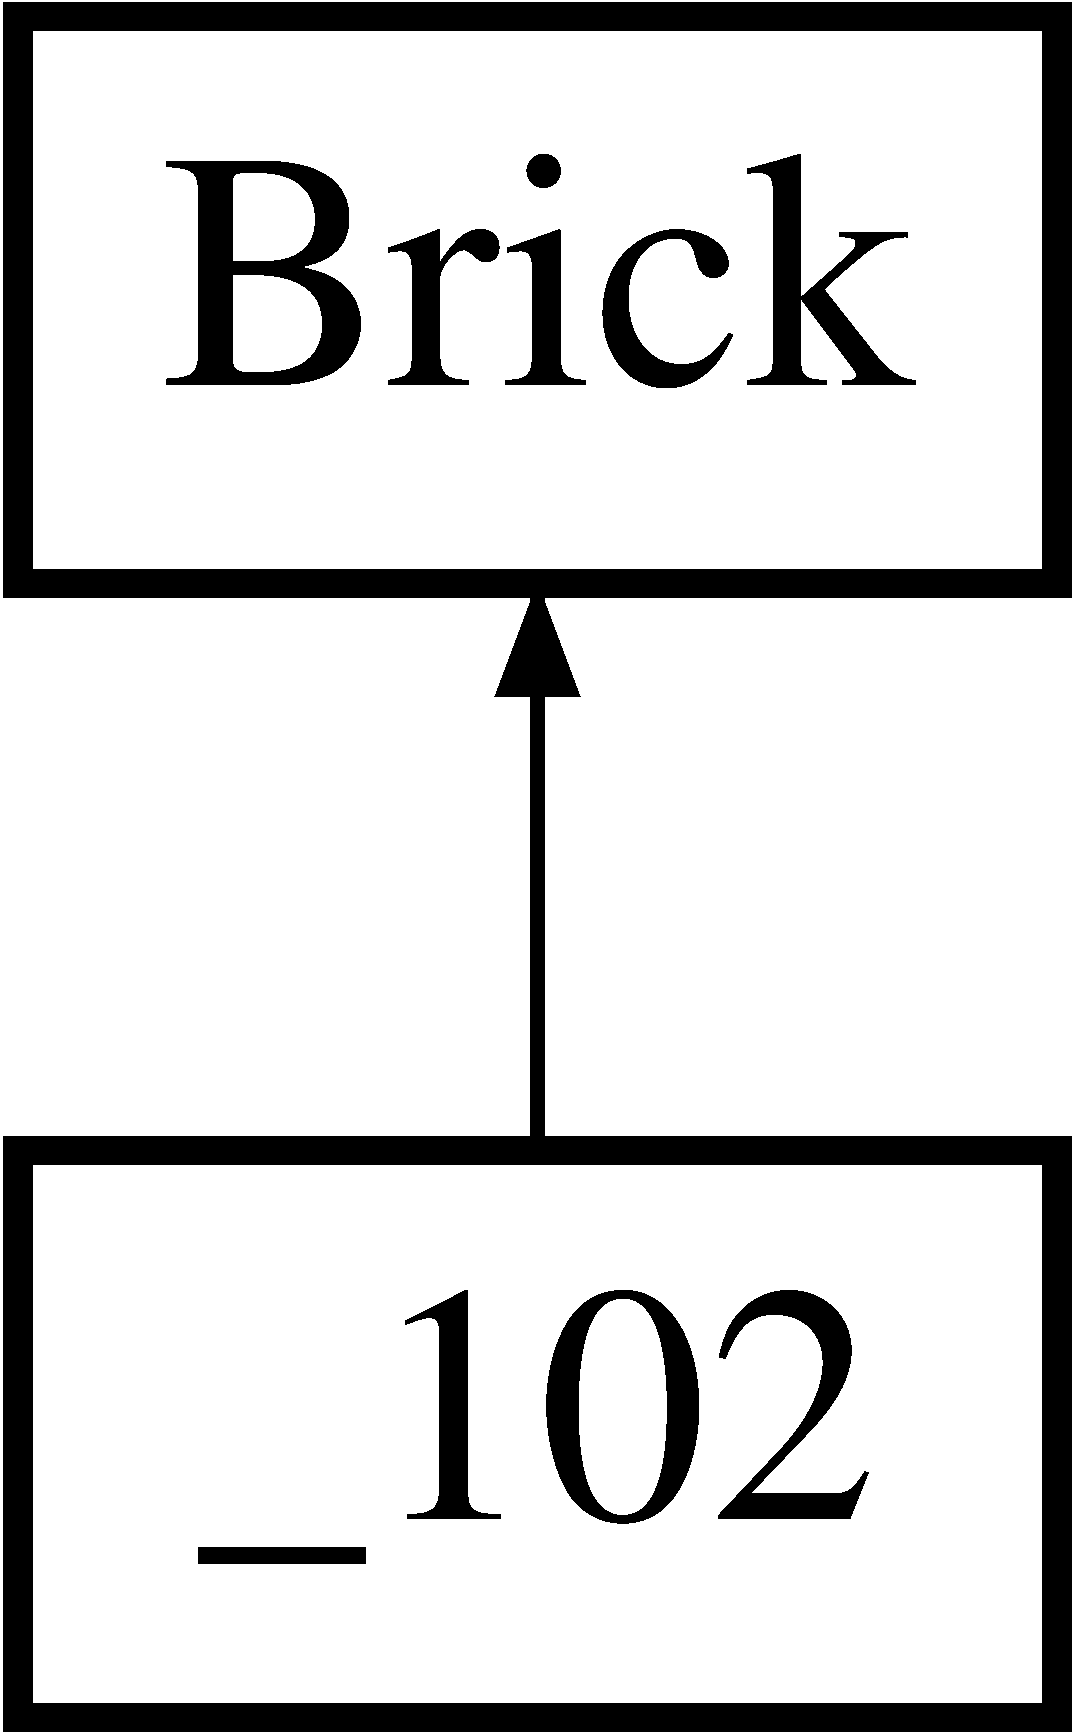
\includegraphics[height=2.000000cm]{d0/dd1/class__102}
\end{center}
\end{figure}
\subsection*{Public Types}
\begin{DoxyCompactItemize}
\item 
enum \hyperlink{class__102_a42c689eb145f12ea5e1959bbc3c8feb9}{Check\+\_\+102\+\_\+key} \{ \\*
\hyperlink{class__102_a42c689eb145f12ea5e1959bbc3c8feb9ab466d28554cd5d20fac2a58e6d309460}{B\+A\+D\+\_\+\+C\+A\+R\+A\+C\+T\+E\+R} = 1, 
\hyperlink{class__102_a42c689eb145f12ea5e1959bbc3c8feb9acd2e260fca6d5654797d46bc4da9c4be}{N\+O\+T\+\_\+\+E\+N\+O\+U\+G\+H\+\_\+\+N\+U\+M\+B\+E\+R\+S} = 2, 
\hyperlink{class__102_a42c689eb145f12ea5e1959bbc3c8feb9a24b75f3235979f8925775f574f37cb56}{N\+O\+\_\+0} = 3, 
\hyperlink{class__102_a42c689eb145f12ea5e1959bbc3c8feb9aa437ed38b4947f5743309d9805eccdc9}{I\+N\+P\+U\+T\+\_\+\+E\+R\+R\+O\+R} = 4, 
\\*
\hyperlink{class__102_a42c689eb145f12ea5e1959bbc3c8feb9a28132c4dfd87b74b2cd3183838e20b88}{G\+O\+O\+D} = 5
 \}
\item 
enum \hyperlink{class__102_a4d2a75091d5c3bedfba6c129a8ed49f1}{Check\+\_\+102\+\_\+base} \{ \\*
\hyperlink{class__102_a4d2a75091d5c3bedfba6c129a8ed49f1ac86693d7acd645a9398cd85fc08adfac}{D\+U\+P\+L\+I\+C\+A\+T\+E} = 1, 
\hyperlink{class__102_a4d2a75091d5c3bedfba6c129a8ed49f1ad6e5f99be534229e2990578c27fadd1b}{N\+O\+\_\+\+N\+E\+G} = 2, 
\hyperlink{class__102_a4d2a75091d5c3bedfba6c129a8ed49f1a5d1bc329f37dee6a2888a1a125ac1411}{B\+A\+D\+\_\+\+C\+A\+R\+A\+C} = 3, 
\hyperlink{class__102_a4d2a75091d5c3bedfba6c129a8ed49f1adb94a359ce07a3ada7bb75972ef18f35}{N\+O\+\_\+\+S\+P\+A\+C\+E} = 4, 
\\*
\hyperlink{class__102_a4d2a75091d5c3bedfba6c129a8ed49f1a33cb65cfcd7f108f863bf5db73102d0b}{O\+K} = 5
 \}
\end{DoxyCompactItemize}
\subsection*{Public Member Functions}
\begin{DoxyCompactItemize}
\item 
std\+::string \hyperlink{class__102_a998fb64410d54af6d71804811f685d09}{dechiffre} (std\+::string \&input)
\item 
std\+::string \hyperlink{class__102_a27ec62277364d81471ed4dbd72e7682b}{chiffre} (std\+::string \&input)
\item 
virtual void \hyperlink{class__102_afb7ce7c2953153f341ad5da9d3a21e9f}{present} ()
\item 
virtual void \hyperlink{class__102_a5fb39b8750033909e60a30facc3f3fe4}{get\+\_\+key} ()
\item 
virtual \hyperlink{class_brick_af32354a4d8d1275db35660a96a2cfa3e}{Brick\+::identity} \hyperlink{class__102_af9dd4029e18d0fc85f8e85ddbe29d7bd}{who} ()
\item 
\hyperlink{class__102_abde9d279babf4486332e9480d4179c5c}{\+\_\+102} ()
\item 
\hyperlink{class__102_ab8d5c40cac7e1d262336166df96087fd}{$\sim$\+\_\+102} ()
\end{DoxyCompactItemize}
\subsection*{Private Member Functions}
\begin{DoxyCompactItemize}
\item 
int \hyperlink{class__102_ad1b8619389086293c1823f2cedac2eb1}{key\+\_\+validator\+\_\+102\+\_\+base} (std\+::string key, const std\+::string lib)
\item 
int \hyperlink{class__102_a78780071832acd65d1fcec91e92d6c49}{input\+\_\+validator} (std\+::string str, const std\+::string lib)
\item 
int \hyperlink{class__102_a168860d1755605cd700310e2ded733c3}{numbers\+\_\+only} (std\+::string \&input)
\item 
int \hyperlink{class__102_a543b704bada4df40e12692bad832da3d}{fast\+\_\+check} (std\+::string \&input)
\item 
int \hyperlink{class__102_ab53cdc3d3ff965ccba78000b897087c1}{write\+\_\+matrix} (Matrix\+Xd \&out, std\+::string tmp)
\item 
int \hyperlink{class__102_a1bff799d8c46a418b49639c938af4ca6}{last\+\_\+check} (Matrix\+Xd \&out)
\item 
void \hyperlink{class__102_a532d1a64f5ac775ea3108a4f0329057e}{matrix\+\_\+input\+\_\+102} (Matrix\+Xd \&out)
\item 
int \hyperlink{class__102_ac06410d4ede0164feea5744ff289b427}{write\+\_\+matrix} (std\+::string tmp)
\item 
int \hyperlink{class__102_ab0abff1bfd0dca0e5d3e47d18ff3231a}{last\+\_\+check} ()
\item 
void \hyperlink{class__102_a1fac5d791ec3f16679d04ada71f6e2c9}{user\+\_\+input\+\_\+to\+\_\+matrix\+\_\+base} (std\+::string \&input)
\item 
\hyperlink{class__102_a42c689eb145f12ea5e1959bbc3c8feb9}{Check\+\_\+102\+\_\+key} \hyperlink{class__102_a5df2cca01360523e282d74ccf7a74661}{key\+\_\+input} (std\+::string \&input)
\item 
\hyperlink{class__102_a4d2a75091d5c3bedfba6c129a8ed49f1}{Check\+\_\+102\+\_\+base} \hyperlink{class__102_a69d2442d8380d8c93ed68a96faddecae}{base\+\_\+input} (std\+::string \&input)
\item 
char \hyperlink{class__102_a5672275701c048a518fcdcf67d671275}{bad\+\_\+carac} ()
\item 
char \hyperlink{class__102_aafd54aef9041a20486af9e9681b5a250}{input\+\_\+validator} (std\+::string \&input)
\end{DoxyCompactItemize}
\subsection*{Private Attributes}
\begin{DoxyCompactItemize}
\item 
char \hyperlink{class__102_ace05d98669089dc84365b756a7555d08}{bad\+\_\+caracter}
\item 
bool \hyperlink{class__102_aedece1a24c9d0ba12efa5e9429eb2de0}{key\+\_\+check}
\item 
std\+::string \hyperlink{class__102_aa3c33241b01dba968530f960bdb21fc3}{base}
\item 
Matrix\+Xd \hyperlink{class__102_a6284519dfd2d04e52a37e265488d05cc}{key\+\_\+matrix}
\item 
Matrix\+Xd \hyperlink{class__102_a2836a7b0f462c1f3ff8b6df7e41420f2}{text\+\_\+matrix}
\end{DoxyCompactItemize}
\subsection*{Additional Inherited Members}


\subsection{Member Enumeration Documentation}
\hypertarget{class__102_a4d2a75091d5c3bedfba6c129a8ed49f1}{}\index{\+\_\+102@{\+\_\+102}!Check\+\_\+102\+\_\+base@{Check\+\_\+102\+\_\+base}}
\index{Check\+\_\+102\+\_\+base@{Check\+\_\+102\+\_\+base}!\+\_\+102@{\+\_\+102}}
\subsubsection[{Check\+\_\+102\+\_\+base}]{\setlength{\rightskip}{0pt plus 5cm}enum {\bf \+\_\+102\+::\+Check\+\_\+102\+\_\+base}}\label{class__102_a4d2a75091d5c3bedfba6c129a8ed49f1}
\begin{Desc}
\item[Enumerator]\par
\begin{description}
\index{D\+U\+P\+L\+I\+C\+A\+T\+E@{D\+U\+P\+L\+I\+C\+A\+T\+E}!\+\_\+102@{\+\_\+102}}\index{\+\_\+102@{\+\_\+102}!D\+U\+P\+L\+I\+C\+A\+T\+E@{D\+U\+P\+L\+I\+C\+A\+T\+E}}\item[{\em 
\hypertarget{class__102_a4d2a75091d5c3bedfba6c129a8ed49f1ac86693d7acd645a9398cd85fc08adfac}{}D\+U\+P\+L\+I\+C\+A\+T\+E\label{class__102_a4d2a75091d5c3bedfba6c129a8ed49f1ac86693d7acd645a9398cd85fc08adfac}
}]\index{N\+O\+\_\+\+N\+E\+G@{N\+O\+\_\+\+N\+E\+G}!\+\_\+102@{\+\_\+102}}\index{\+\_\+102@{\+\_\+102}!N\+O\+\_\+\+N\+E\+G@{N\+O\+\_\+\+N\+E\+G}}\item[{\em 
\hypertarget{class__102_a4d2a75091d5c3bedfba6c129a8ed49f1ad6e5f99be534229e2990578c27fadd1b}{}N\+O\+\_\+\+N\+E\+G\label{class__102_a4d2a75091d5c3bedfba6c129a8ed49f1ad6e5f99be534229e2990578c27fadd1b}
}]\index{B\+A\+D\+\_\+\+C\+A\+R\+A\+C@{B\+A\+D\+\_\+\+C\+A\+R\+A\+C}!\+\_\+102@{\+\_\+102}}\index{\+\_\+102@{\+\_\+102}!B\+A\+D\+\_\+\+C\+A\+R\+A\+C@{B\+A\+D\+\_\+\+C\+A\+R\+A\+C}}\item[{\em 
\hypertarget{class__102_a4d2a75091d5c3bedfba6c129a8ed49f1a5d1bc329f37dee6a2888a1a125ac1411}{}B\+A\+D\+\_\+\+C\+A\+R\+A\+C\label{class__102_a4d2a75091d5c3bedfba6c129a8ed49f1a5d1bc329f37dee6a2888a1a125ac1411}
}]\index{N\+O\+\_\+\+S\+P\+A\+C\+E@{N\+O\+\_\+\+S\+P\+A\+C\+E}!\+\_\+102@{\+\_\+102}}\index{\+\_\+102@{\+\_\+102}!N\+O\+\_\+\+S\+P\+A\+C\+E@{N\+O\+\_\+\+S\+P\+A\+C\+E}}\item[{\em 
\hypertarget{class__102_a4d2a75091d5c3bedfba6c129a8ed49f1adb94a359ce07a3ada7bb75972ef18f35}{}N\+O\+\_\+\+S\+P\+A\+C\+E\label{class__102_a4d2a75091d5c3bedfba6c129a8ed49f1adb94a359ce07a3ada7bb75972ef18f35}
}]\index{O\+K@{O\+K}!\+\_\+102@{\+\_\+102}}\index{\+\_\+102@{\+\_\+102}!O\+K@{O\+K}}\item[{\em 
\hypertarget{class__102_a4d2a75091d5c3bedfba6c129a8ed49f1a33cb65cfcd7f108f863bf5db73102d0b}{}O\+K\label{class__102_a4d2a75091d5c3bedfba6c129a8ed49f1a33cb65cfcd7f108f863bf5db73102d0b}
}]\end{description}
\end{Desc}
\hypertarget{class__102_a42c689eb145f12ea5e1959bbc3c8feb9}{}\index{\+\_\+102@{\+\_\+102}!Check\+\_\+102\+\_\+key@{Check\+\_\+102\+\_\+key}}
\index{Check\+\_\+102\+\_\+key@{Check\+\_\+102\+\_\+key}!\+\_\+102@{\+\_\+102}}
\subsubsection[{Check\+\_\+102\+\_\+key}]{\setlength{\rightskip}{0pt plus 5cm}enum {\bf \+\_\+102\+::\+Check\+\_\+102\+\_\+key}}\label{class__102_a42c689eb145f12ea5e1959bbc3c8feb9}
\begin{Desc}
\item[Enumerator]\par
\begin{description}
\index{B\+A\+D\+\_\+\+C\+A\+R\+A\+C\+T\+E\+R@{B\+A\+D\+\_\+\+C\+A\+R\+A\+C\+T\+E\+R}!\+\_\+102@{\+\_\+102}}\index{\+\_\+102@{\+\_\+102}!B\+A\+D\+\_\+\+C\+A\+R\+A\+C\+T\+E\+R@{B\+A\+D\+\_\+\+C\+A\+R\+A\+C\+T\+E\+R}}\item[{\em 
\hypertarget{class__102_a42c689eb145f12ea5e1959bbc3c8feb9ab466d28554cd5d20fac2a58e6d309460}{}B\+A\+D\+\_\+\+C\+A\+R\+A\+C\+T\+E\+R\label{class__102_a42c689eb145f12ea5e1959bbc3c8feb9ab466d28554cd5d20fac2a58e6d309460}
}]\index{N\+O\+T\+\_\+\+E\+N\+O\+U\+G\+H\+\_\+\+N\+U\+M\+B\+E\+R\+S@{N\+O\+T\+\_\+\+E\+N\+O\+U\+G\+H\+\_\+\+N\+U\+M\+B\+E\+R\+S}!\+\_\+102@{\+\_\+102}}\index{\+\_\+102@{\+\_\+102}!N\+O\+T\+\_\+\+E\+N\+O\+U\+G\+H\+\_\+\+N\+U\+M\+B\+E\+R\+S@{N\+O\+T\+\_\+\+E\+N\+O\+U\+G\+H\+\_\+\+N\+U\+M\+B\+E\+R\+S}}\item[{\em 
\hypertarget{class__102_a42c689eb145f12ea5e1959bbc3c8feb9acd2e260fca6d5654797d46bc4da9c4be}{}N\+O\+T\+\_\+\+E\+N\+O\+U\+G\+H\+\_\+\+N\+U\+M\+B\+E\+R\+S\label{class__102_a42c689eb145f12ea5e1959bbc3c8feb9acd2e260fca6d5654797d46bc4da9c4be}
}]\index{N\+O\+\_\+0@{N\+O\+\_\+0}!\+\_\+102@{\+\_\+102}}\index{\+\_\+102@{\+\_\+102}!N\+O\+\_\+0@{N\+O\+\_\+0}}\item[{\em 
\hypertarget{class__102_a42c689eb145f12ea5e1959bbc3c8feb9a24b75f3235979f8925775f574f37cb56}{}N\+O\+\_\+0\label{class__102_a42c689eb145f12ea5e1959bbc3c8feb9a24b75f3235979f8925775f574f37cb56}
}]\index{I\+N\+P\+U\+T\+\_\+\+E\+R\+R\+O\+R@{I\+N\+P\+U\+T\+\_\+\+E\+R\+R\+O\+R}!\+\_\+102@{\+\_\+102}}\index{\+\_\+102@{\+\_\+102}!I\+N\+P\+U\+T\+\_\+\+E\+R\+R\+O\+R@{I\+N\+P\+U\+T\+\_\+\+E\+R\+R\+O\+R}}\item[{\em 
\hypertarget{class__102_a42c689eb145f12ea5e1959bbc3c8feb9aa437ed38b4947f5743309d9805eccdc9}{}I\+N\+P\+U\+T\+\_\+\+E\+R\+R\+O\+R\label{class__102_a42c689eb145f12ea5e1959bbc3c8feb9aa437ed38b4947f5743309d9805eccdc9}
}]\index{G\+O\+O\+D@{G\+O\+O\+D}!\+\_\+102@{\+\_\+102}}\index{\+\_\+102@{\+\_\+102}!G\+O\+O\+D@{G\+O\+O\+D}}\item[{\em 
\hypertarget{class__102_a42c689eb145f12ea5e1959bbc3c8feb9a28132c4dfd87b74b2cd3183838e20b88}{}G\+O\+O\+D\label{class__102_a42c689eb145f12ea5e1959bbc3c8feb9a28132c4dfd87b74b2cd3183838e20b88}
}]\end{description}
\end{Desc}


\subsection{Constructor \& Destructor Documentation}
\hypertarget{class__102_abde9d279babf4486332e9480d4179c5c}{}\index{\+\_\+102@{\+\_\+102}!\+\_\+102@{\+\_\+102}}
\index{\+\_\+102@{\+\_\+102}!\+\_\+102@{\+\_\+102}}
\subsubsection[{\+\_\+102()}]{\setlength{\rightskip}{0pt plus 5cm}\+\_\+102\+::\+\_\+102 (
\begin{DoxyParamCaption}
{}
\end{DoxyParamCaption}
)}\label{class__102_abde9d279babf4486332e9480d4179c5c}
\hypertarget{class__102_ab8d5c40cac7e1d262336166df96087fd}{}\index{\+\_\+102@{\+\_\+102}!````~\+\_\+102@{$\sim$\+\_\+102}}
\index{````~\+\_\+102@{$\sim$\+\_\+102}!\+\_\+102@{\+\_\+102}}
\subsubsection[{$\sim$\+\_\+102()}]{\setlength{\rightskip}{0pt plus 5cm}\+\_\+102\+::$\sim$\+\_\+102 (
\begin{DoxyParamCaption}
{}
\end{DoxyParamCaption}
)}\label{class__102_ab8d5c40cac7e1d262336166df96087fd}


\subsection{Member Function Documentation}
\hypertarget{class__102_a5672275701c048a518fcdcf67d671275}{}\index{\+\_\+102@{\+\_\+102}!bad\+\_\+carac@{bad\+\_\+carac}}
\index{bad\+\_\+carac@{bad\+\_\+carac}!\+\_\+102@{\+\_\+102}}
\subsubsection[{bad\+\_\+carac()}]{\setlength{\rightskip}{0pt plus 5cm}char \+\_\+102\+::bad\+\_\+carac (
\begin{DoxyParamCaption}
{}
\end{DoxyParamCaption}
)\hspace{0.3cm}{\ttfamily [private]}}\label{class__102_a5672275701c048a518fcdcf67d671275}
\hypertarget{class__102_a69d2442d8380d8c93ed68a96faddecae}{}\index{\+\_\+102@{\+\_\+102}!base\+\_\+input@{base\+\_\+input}}
\index{base\+\_\+input@{base\+\_\+input}!\+\_\+102@{\+\_\+102}}
\subsubsection[{base\+\_\+input(std\+::string \&input)}]{\setlength{\rightskip}{0pt plus 5cm}{\bf \+\_\+102\+::\+Check\+\_\+102\+\_\+base} \+\_\+102\+::base\+\_\+input (
\begin{DoxyParamCaption}
\item[{std\+::string \&}]{input}
\end{DoxyParamCaption}
)\hspace{0.3cm}{\ttfamily [private]}}\label{class__102_a69d2442d8380d8c93ed68a96faddecae}
\hypertarget{class__102_a27ec62277364d81471ed4dbd72e7682b}{}\index{\+\_\+102@{\+\_\+102}!chiffre@{chiffre}}
\index{chiffre@{chiffre}!\+\_\+102@{\+\_\+102}}
\subsubsection[{chiffre(std\+::string \&input)}]{\setlength{\rightskip}{0pt plus 5cm}std\+::string \+\_\+102\+::chiffre (
\begin{DoxyParamCaption}
\item[{std\+::string \&}]{input}
\end{DoxyParamCaption}
)\hspace{0.3cm}{\ttfamily [virtual]}}\label{class__102_a27ec62277364d81471ed4dbd72e7682b}


Implements \hyperlink{class_brick_a1cddb42fe77c9b6d140004d01ff7ab5b}{Brick}.

\hypertarget{class__102_a998fb64410d54af6d71804811f685d09}{}\index{\+\_\+102@{\+\_\+102}!dechiffre@{dechiffre}}
\index{dechiffre@{dechiffre}!\+\_\+102@{\+\_\+102}}
\subsubsection[{dechiffre(std\+::string \&input)}]{\setlength{\rightskip}{0pt plus 5cm}std\+::string \+\_\+102\+::dechiffre (
\begin{DoxyParamCaption}
\item[{std\+::string \&}]{input}
\end{DoxyParamCaption}
)\hspace{0.3cm}{\ttfamily [virtual]}}\label{class__102_a998fb64410d54af6d71804811f685d09}


Implements \hyperlink{class_brick_afa3a68ba4f4babecadc6dfd05a2d2040}{Brick}.

\hypertarget{class__102_a543b704bada4df40e12692bad832da3d}{}\index{\+\_\+102@{\+\_\+102}!fast\+\_\+check@{fast\+\_\+check}}
\index{fast\+\_\+check@{fast\+\_\+check}!\+\_\+102@{\+\_\+102}}
\subsubsection[{fast\+\_\+check(std\+::string \&input)}]{\setlength{\rightskip}{0pt plus 5cm}int \+\_\+102\+::fast\+\_\+check (
\begin{DoxyParamCaption}
\item[{std\+::string \&}]{input}
\end{DoxyParamCaption}
)\hspace{0.3cm}{\ttfamily [private]}}\label{class__102_a543b704bada4df40e12692bad832da3d}
\hypertarget{class__102_a5fb39b8750033909e60a30facc3f3fe4}{}\index{\+\_\+102@{\+\_\+102}!get\+\_\+key@{get\+\_\+key}}
\index{get\+\_\+key@{get\+\_\+key}!\+\_\+102@{\+\_\+102}}
\subsubsection[{get\+\_\+key()}]{\setlength{\rightskip}{0pt plus 5cm}void \+\_\+102\+::get\+\_\+key (
\begin{DoxyParamCaption}
{}
\end{DoxyParamCaption}
)\hspace{0.3cm}{\ttfamily [virtual]}}\label{class__102_a5fb39b8750033909e60a30facc3f3fe4}


Implements \hyperlink{class_brick_aeec3d78d8d03e207b4154ff06f637bbe}{Brick}.

\hypertarget{class__102_a78780071832acd65d1fcec91e92d6c49}{}\index{\+\_\+102@{\+\_\+102}!input\+\_\+validator@{input\+\_\+validator}}
\index{input\+\_\+validator@{input\+\_\+validator}!\+\_\+102@{\+\_\+102}}
\subsubsection[{input\+\_\+validator(std\+::string str, const std\+::string lib)}]{\setlength{\rightskip}{0pt plus 5cm}int \+\_\+102\+::input\+\_\+validator (
\begin{DoxyParamCaption}
\item[{std\+::string}]{str, }
\item[{const std\+::string}]{lib}
\end{DoxyParamCaption}
)\hspace{0.3cm}{\ttfamily [private]}}\label{class__102_a78780071832acd65d1fcec91e92d6c49}
\hypertarget{class__102_aafd54aef9041a20486af9e9681b5a250}{}\index{\+\_\+102@{\+\_\+102}!input\+\_\+validator@{input\+\_\+validator}}
\index{input\+\_\+validator@{input\+\_\+validator}!\+\_\+102@{\+\_\+102}}
\subsubsection[{input\+\_\+validator(std\+::string \&input)}]{\setlength{\rightskip}{0pt plus 5cm}char \+\_\+102\+::input\+\_\+validator (
\begin{DoxyParamCaption}
\item[{std\+::string \&}]{input}
\end{DoxyParamCaption}
)\hspace{0.3cm}{\ttfamily [private]}}\label{class__102_aafd54aef9041a20486af9e9681b5a250}
\hypertarget{class__102_a5df2cca01360523e282d74ccf7a74661}{}\index{\+\_\+102@{\+\_\+102}!key\+\_\+input@{key\+\_\+input}}
\index{key\+\_\+input@{key\+\_\+input}!\+\_\+102@{\+\_\+102}}
\subsubsection[{key\+\_\+input(std\+::string \&input)}]{\setlength{\rightskip}{0pt plus 5cm}{\bf \+\_\+102\+::\+Check\+\_\+102\+\_\+key} \+\_\+102\+::key\+\_\+input (
\begin{DoxyParamCaption}
\item[{std\+::string \&}]{input}
\end{DoxyParamCaption}
)\hspace{0.3cm}{\ttfamily [private]}}\label{class__102_a5df2cca01360523e282d74ccf7a74661}
\hypertarget{class__102_ad1b8619389086293c1823f2cedac2eb1}{}\index{\+\_\+102@{\+\_\+102}!key\+\_\+validator\+\_\+102\+\_\+base@{key\+\_\+validator\+\_\+102\+\_\+base}}
\index{key\+\_\+validator\+\_\+102\+\_\+base@{key\+\_\+validator\+\_\+102\+\_\+base}!\+\_\+102@{\+\_\+102}}
\subsubsection[{key\+\_\+validator\+\_\+102\+\_\+base(std\+::string key, const std\+::string lib)}]{\setlength{\rightskip}{0pt plus 5cm}int \+\_\+102\+::key\+\_\+validator\+\_\+102\+\_\+base (
\begin{DoxyParamCaption}
\item[{std\+::string}]{key, }
\item[{const std\+::string}]{lib}
\end{DoxyParamCaption}
)\hspace{0.3cm}{\ttfamily [private]}}\label{class__102_ad1b8619389086293c1823f2cedac2eb1}
\hypertarget{class__102_a1bff799d8c46a418b49639c938af4ca6}{}\index{\+\_\+102@{\+\_\+102}!last\+\_\+check@{last\+\_\+check}}
\index{last\+\_\+check@{last\+\_\+check}!\+\_\+102@{\+\_\+102}}
\subsubsection[{last\+\_\+check(\+Matrix\+Xd \&out)}]{\setlength{\rightskip}{0pt plus 5cm}int \+\_\+102\+::last\+\_\+check (
\begin{DoxyParamCaption}
\item[{Matrix\+Xd \&}]{out}
\end{DoxyParamCaption}
)\hspace{0.3cm}{\ttfamily [private]}}\label{class__102_a1bff799d8c46a418b49639c938af4ca6}
\hypertarget{class__102_ab0abff1bfd0dca0e5d3e47d18ff3231a}{}\index{\+\_\+102@{\+\_\+102}!last\+\_\+check@{last\+\_\+check}}
\index{last\+\_\+check@{last\+\_\+check}!\+\_\+102@{\+\_\+102}}
\subsubsection[{last\+\_\+check()}]{\setlength{\rightskip}{0pt plus 5cm}int \+\_\+102\+::last\+\_\+check (
\begin{DoxyParamCaption}
{}
\end{DoxyParamCaption}
)\hspace{0.3cm}{\ttfamily [private]}}\label{class__102_ab0abff1bfd0dca0e5d3e47d18ff3231a}
\hypertarget{class__102_a532d1a64f5ac775ea3108a4f0329057e}{}\index{\+\_\+102@{\+\_\+102}!matrix\+\_\+input\+\_\+102@{matrix\+\_\+input\+\_\+102}}
\index{matrix\+\_\+input\+\_\+102@{matrix\+\_\+input\+\_\+102}!\+\_\+102@{\+\_\+102}}
\subsubsection[{matrix\+\_\+input\+\_\+102(\+Matrix\+Xd \&out)}]{\setlength{\rightskip}{0pt plus 5cm}void \+\_\+102\+::matrix\+\_\+input\+\_\+102 (
\begin{DoxyParamCaption}
\item[{Matrix\+Xd \&}]{out}
\end{DoxyParamCaption}
)\hspace{0.3cm}{\ttfamily [private]}}\label{class__102_a532d1a64f5ac775ea3108a4f0329057e}
\hypertarget{class__102_a168860d1755605cd700310e2ded733c3}{}\index{\+\_\+102@{\+\_\+102}!numbers\+\_\+only@{numbers\+\_\+only}}
\index{numbers\+\_\+only@{numbers\+\_\+only}!\+\_\+102@{\+\_\+102}}
\subsubsection[{numbers\+\_\+only(std\+::string \&input)}]{\setlength{\rightskip}{0pt plus 5cm}int \+\_\+102\+::numbers\+\_\+only (
\begin{DoxyParamCaption}
\item[{std\+::string \&}]{input}
\end{DoxyParamCaption}
)\hspace{0.3cm}{\ttfamily [private]}}\label{class__102_a168860d1755605cd700310e2ded733c3}
\hypertarget{class__102_afb7ce7c2953153f341ad5da9d3a21e9f}{}\index{\+\_\+102@{\+\_\+102}!present@{present}}
\index{present@{present}!\+\_\+102@{\+\_\+102}}
\subsubsection[{present()}]{\setlength{\rightskip}{0pt plus 5cm}void \+\_\+102\+::present (
\begin{DoxyParamCaption}
{}
\end{DoxyParamCaption}
)\hspace{0.3cm}{\ttfamily [virtual]}}\label{class__102_afb7ce7c2953153f341ad5da9d3a21e9f}


Implements \hyperlink{class_brick_aa1e9b549787dedc030860f8c75482c8c}{Brick}.

\hypertarget{class__102_a1fac5d791ec3f16679d04ada71f6e2c9}{}\index{\+\_\+102@{\+\_\+102}!user\+\_\+input\+\_\+to\+\_\+matrix\+\_\+base@{user\+\_\+input\+\_\+to\+\_\+matrix\+\_\+base}}
\index{user\+\_\+input\+\_\+to\+\_\+matrix\+\_\+base@{user\+\_\+input\+\_\+to\+\_\+matrix\+\_\+base}!\+\_\+102@{\+\_\+102}}
\subsubsection[{user\+\_\+input\+\_\+to\+\_\+matrix\+\_\+base(std\+::string \&input)}]{\setlength{\rightskip}{0pt plus 5cm}void \+\_\+102\+::user\+\_\+input\+\_\+to\+\_\+matrix\+\_\+base (
\begin{DoxyParamCaption}
\item[{std\+::string \&}]{input}
\end{DoxyParamCaption}
)\hspace{0.3cm}{\ttfamily [private]}}\label{class__102_a1fac5d791ec3f16679d04ada71f6e2c9}
\hypertarget{class__102_af9dd4029e18d0fc85f8e85ddbe29d7bd}{}\index{\+\_\+102@{\+\_\+102}!who@{who}}
\index{who@{who}!\+\_\+102@{\+\_\+102}}
\subsubsection[{who()}]{\setlength{\rightskip}{0pt plus 5cm}{\bf Brick\+::identity} \+\_\+102\+::who (
\begin{DoxyParamCaption}
{}
\end{DoxyParamCaption}
)\hspace{0.3cm}{\ttfamily [virtual]}}\label{class__102_af9dd4029e18d0fc85f8e85ddbe29d7bd}


Implements \hyperlink{class_brick_af6ba737fda1fda2d3fba50de23cbaff0}{Brick}.

\hypertarget{class__102_ab53cdc3d3ff965ccba78000b897087c1}{}\index{\+\_\+102@{\+\_\+102}!write\+\_\+matrix@{write\+\_\+matrix}}
\index{write\+\_\+matrix@{write\+\_\+matrix}!\+\_\+102@{\+\_\+102}}
\subsubsection[{write\+\_\+matrix(\+Matrix\+Xd \&out, std\+::string tmp)}]{\setlength{\rightskip}{0pt plus 5cm}int \+\_\+102\+::write\+\_\+matrix (
\begin{DoxyParamCaption}
\item[{Matrix\+Xd \&}]{out, }
\item[{std\+::string}]{tmp}
\end{DoxyParamCaption}
)\hspace{0.3cm}{\ttfamily [private]}}\label{class__102_ab53cdc3d3ff965ccba78000b897087c1}
\hypertarget{class__102_ac06410d4ede0164feea5744ff289b427}{}\index{\+\_\+102@{\+\_\+102}!write\+\_\+matrix@{write\+\_\+matrix}}
\index{write\+\_\+matrix@{write\+\_\+matrix}!\+\_\+102@{\+\_\+102}}
\subsubsection[{write\+\_\+matrix(std\+::string tmp)}]{\setlength{\rightskip}{0pt plus 5cm}int \+\_\+102\+::write\+\_\+matrix (
\begin{DoxyParamCaption}
\item[{std\+::string}]{tmp}
\end{DoxyParamCaption}
)\hspace{0.3cm}{\ttfamily [private]}}\label{class__102_ac06410d4ede0164feea5744ff289b427}


\subsection{Member Data Documentation}
\hypertarget{class__102_ace05d98669089dc84365b756a7555d08}{}\index{\+\_\+102@{\+\_\+102}!bad\+\_\+caracter@{bad\+\_\+caracter}}
\index{bad\+\_\+caracter@{bad\+\_\+caracter}!\+\_\+102@{\+\_\+102}}
\subsubsection[{bad\+\_\+caracter}]{\setlength{\rightskip}{0pt plus 5cm}char \+\_\+102\+::bad\+\_\+caracter\hspace{0.3cm}{\ttfamily [private]}}\label{class__102_ace05d98669089dc84365b756a7555d08}
\hypertarget{class__102_aa3c33241b01dba968530f960bdb21fc3}{}\index{\+\_\+102@{\+\_\+102}!base@{base}}
\index{base@{base}!\+\_\+102@{\+\_\+102}}
\subsubsection[{base}]{\setlength{\rightskip}{0pt plus 5cm}std\+::string \+\_\+102\+::base\hspace{0.3cm}{\ttfamily [private]}}\label{class__102_aa3c33241b01dba968530f960bdb21fc3}
\hypertarget{class__102_aedece1a24c9d0ba12efa5e9429eb2de0}{}\index{\+\_\+102@{\+\_\+102}!key\+\_\+check@{key\+\_\+check}}
\index{key\+\_\+check@{key\+\_\+check}!\+\_\+102@{\+\_\+102}}
\subsubsection[{key\+\_\+check}]{\setlength{\rightskip}{0pt plus 5cm}bool \+\_\+102\+::key\+\_\+check\hspace{0.3cm}{\ttfamily [private]}}\label{class__102_aedece1a24c9d0ba12efa5e9429eb2de0}
\hypertarget{class__102_a6284519dfd2d04e52a37e265488d05cc}{}\index{\+\_\+102@{\+\_\+102}!key\+\_\+matrix@{key\+\_\+matrix}}
\index{key\+\_\+matrix@{key\+\_\+matrix}!\+\_\+102@{\+\_\+102}}
\subsubsection[{key\+\_\+matrix}]{\setlength{\rightskip}{0pt plus 5cm}Matrix\+Xd \+\_\+102\+::key\+\_\+matrix\hspace{0.3cm}{\ttfamily [private]}}\label{class__102_a6284519dfd2d04e52a37e265488d05cc}
\hypertarget{class__102_a2836a7b0f462c1f3ff8b6df7e41420f2}{}\index{\+\_\+102@{\+\_\+102}!text\+\_\+matrix@{text\+\_\+matrix}}
\index{text\+\_\+matrix@{text\+\_\+matrix}!\+\_\+102@{\+\_\+102}}
\subsubsection[{text\+\_\+matrix}]{\setlength{\rightskip}{0pt plus 5cm}Matrix\+Xd \+\_\+102\+::text\+\_\+matrix\hspace{0.3cm}{\ttfamily [private]}}\label{class__102_a2836a7b0f462c1f3ff8b6df7e41420f2}


The documentation for this class was generated from the following files\+:\begin{DoxyCompactItemize}
\item 
includes/core/\hyperlink{102_8hpp}{102.\+hpp}\item 
sources/core/bricks/102/\hyperlink{__102__brick__functions_8cpp}{\+\_\+102\+\_\+brick\+\_\+functions.\+cpp}\item 
sources/core/bricks/102/\hyperlink{__102__chiffre__dechiffre_8cpp}{\+\_\+102\+\_\+chiffre\+\_\+dechiffre.\+cpp}\item 
sources/core/bricks/102/\hyperlink{__102__input_8cpp}{\+\_\+102\+\_\+input.\+cpp}\item 
sources/core/bricks/102/\hyperlink{__102__key__input_8cpp}{\+\_\+102\+\_\+key\+\_\+input.\+cpp}\item 
sources/core/bricks/102/\hyperlink{__102__matrix__input_8cpp}{\+\_\+102\+\_\+matrix\+\_\+input.\+cpp}\item 
sources/core/bricks/102/\hyperlink{__102__utilitaires_8cpp}{\+\_\+102\+\_\+utilitaires.\+cpp}\end{DoxyCompactItemize}

\hypertarget{class_brick}{}\section{Brick Class Reference}
\label{class_brick}\index{Brick@{Brick}}


{\ttfamily \#include $<$Brick.\+hpp$>$}

Inheritance diagram for Brick\+:\begin{figure}[H]
\begin{center}
\leavevmode
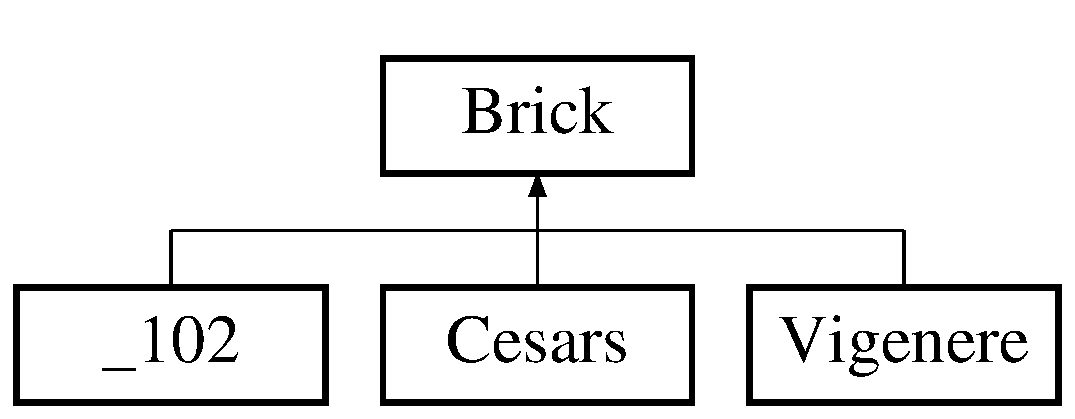
\includegraphics[height=2.000000cm]{d6/db9/class_brick}
\end{center}
\end{figure}
\subsection*{Public Types}
\begin{DoxyCompactItemize}
\item 
enum \hyperlink{class_brick_af32354a4d8d1275db35660a96a2cfa3e}{identity} \{ \\*
\hyperlink{class_brick_af32354a4d8d1275db35660a96a2cfa3eaf72c0102bd6b6f8f6f835ab490e1cd16}{C}, 
\hyperlink{class_brick_af32354a4d8d1275db35660a96a2cfa3ea35e09d567643db467ad9edfbb0574acc}{V}, 
\hyperlink{class_brick_af32354a4d8d1275db35660a96a2cfa3ea5a5f31986f285ab13f2cf5cd3022c5e2}{V3\+D}, 
\hyperlink{class_brick_af32354a4d8d1275db35660a96a2cfa3ea2cb1166fdee35603cf114800f3a101ef}{\+\_\+102}, 
\\*
\hyperlink{class_brick_af32354a4d8d1275db35660a96a2cfa3ea715641459a1350fed267ec501d8c27a5}{\+\_\+10\+X}, 
\hyperlink{class_brick_af32354a4d8d1275db35660a96a2cfa3ea33b4768f26d523132928e96355b5540f}{D}, 
\hyperlink{class_brick_af32354a4d8d1275db35660a96a2cfa3ea961676a52649c6acfe35d6df2b89bbbf}{S\+D}
 \}
\end{DoxyCompactItemize}
\subsection*{Public Member Functions}
\begin{DoxyCompactItemize}
\item 
void \hyperlink{class_brick_a3e683a0fa3648b5a758b6f12d57365ab}{get\+\_\+lib} (int lib)
\item 
virtual void \hyperlink{class_brick_aa1e9b549787dedc030860f8c75482c8c}{present} ()=0
\item 
virtual void \hyperlink{class_brick_aeec3d78d8d03e207b4154ff06f637bbe}{get\+\_\+key} ()=0
\item 
virtual \hyperlink{class_brick_af32354a4d8d1275db35660a96a2cfa3e}{identity} \hyperlink{class_brick_af6ba737fda1fda2d3fba50de23cbaff0}{who} ()=0
\item 
virtual std\+::string \hyperlink{class_brick_a1cddb42fe77c9b6d140004d01ff7ab5b}{chiffre} (std\+::string \&input)=0
\item 
virtual std\+::string \hyperlink{class_brick_afa3a68ba4f4babecadc6dfd05a2d2040}{dechiffre} (std\+::string \&input)=0
\item 
\hyperlink{class_brick_aa29d678c3d901c7b18cbc3a27a51be17}{Brick} ()
\item 
virtual \hyperlink{class_brick_a0e27476ccaeaed1d61a06bddf247c8ee}{$\sim$\+Brick} ()
\end{DoxyCompactItemize}
\subsection*{Protected Attributes}
\begin{DoxyCompactItemize}
\item 
const char $\ast$ \hyperlink{class_brick_ae1175c82acc7e4e74a4cbe27ba75ae66}{\+\_\+lib}
\item 
int \hyperlink{class_brick_a990cb3ac8d11d28aa1fa68a4583ed704}{\+\_\+lib\+\_\+size}
\end{DoxyCompactItemize}


\subsection{Member Enumeration Documentation}
\hypertarget{class_brick_af32354a4d8d1275db35660a96a2cfa3e}{}\index{Brick@{Brick}!identity@{identity}}
\index{identity@{identity}!Brick@{Brick}}
\subsubsection[{identity}]{\setlength{\rightskip}{0pt plus 5cm}enum {\bf Brick\+::identity}}\label{class_brick_af32354a4d8d1275db35660a96a2cfa3e}
\begin{Desc}
\item[Enumerator]\par
\begin{description}
\index{C@{C}!Brick@{Brick}}\index{Brick@{Brick}!C@{C}}\item[{\em 
\hypertarget{class_brick_af32354a4d8d1275db35660a96a2cfa3eaf72c0102bd6b6f8f6f835ab490e1cd16}{}C\label{class_brick_af32354a4d8d1275db35660a96a2cfa3eaf72c0102bd6b6f8f6f835ab490e1cd16}
}]\index{V@{V}!Brick@{Brick}}\index{Brick@{Brick}!V@{V}}\item[{\em 
\hypertarget{class_brick_af32354a4d8d1275db35660a96a2cfa3ea35e09d567643db467ad9edfbb0574acc}{}V\label{class_brick_af32354a4d8d1275db35660a96a2cfa3ea35e09d567643db467ad9edfbb0574acc}
}]\index{V3\+D@{V3\+D}!Brick@{Brick}}\index{Brick@{Brick}!V3\+D@{V3\+D}}\item[{\em 
\hypertarget{class_brick_af32354a4d8d1275db35660a96a2cfa3ea5a5f31986f285ab13f2cf5cd3022c5e2}{}V3\+D\label{class_brick_af32354a4d8d1275db35660a96a2cfa3ea5a5f31986f285ab13f2cf5cd3022c5e2}
}]\index{\+\_\+102@{\+\_\+102}!Brick@{Brick}}\index{Brick@{Brick}!\+\_\+102@{\+\_\+102}}\item[{\em 
\hypertarget{class_brick_af32354a4d8d1275db35660a96a2cfa3ea2cb1166fdee35603cf114800f3a101ef}{}\+\_\+102\label{class_brick_af32354a4d8d1275db35660a96a2cfa3ea2cb1166fdee35603cf114800f3a101ef}
}]\index{\+\_\+10\+X@{\+\_\+10\+X}!Brick@{Brick}}\index{Brick@{Brick}!\+\_\+10\+X@{\+\_\+10\+X}}\item[{\em 
\hypertarget{class_brick_af32354a4d8d1275db35660a96a2cfa3ea715641459a1350fed267ec501d8c27a5}{}\+\_\+10\+X\label{class_brick_af32354a4d8d1275db35660a96a2cfa3ea715641459a1350fed267ec501d8c27a5}
}]\index{D@{D}!Brick@{Brick}}\index{Brick@{Brick}!D@{D}}\item[{\em 
\hypertarget{class_brick_af32354a4d8d1275db35660a96a2cfa3ea33b4768f26d523132928e96355b5540f}{}D\label{class_brick_af32354a4d8d1275db35660a96a2cfa3ea33b4768f26d523132928e96355b5540f}
}]\index{S\+D@{S\+D}!Brick@{Brick}}\index{Brick@{Brick}!S\+D@{S\+D}}\item[{\em 
\hypertarget{class_brick_af32354a4d8d1275db35660a96a2cfa3ea961676a52649c6acfe35d6df2b89bbbf}{}S\+D\label{class_brick_af32354a4d8d1275db35660a96a2cfa3ea961676a52649c6acfe35d6df2b89bbbf}
}]\end{description}
\end{Desc}


\subsection{Constructor \& Destructor Documentation}
\hypertarget{class_brick_aa29d678c3d901c7b18cbc3a27a51be17}{}\index{Brick@{Brick}!Brick@{Brick}}
\index{Brick@{Brick}!Brick@{Brick}}
\subsubsection[{Brick()}]{\setlength{\rightskip}{0pt plus 5cm}Brick\+::\+Brick (
\begin{DoxyParamCaption}
{}
\end{DoxyParamCaption}
)}\label{class_brick_aa29d678c3d901c7b18cbc3a27a51be17}
\hypertarget{class_brick_a0e27476ccaeaed1d61a06bddf247c8ee}{}\index{Brick@{Brick}!````~Brick@{$\sim$\+Brick}}
\index{````~Brick@{$\sim$\+Brick}!Brick@{Brick}}
\subsubsection[{$\sim$\+Brick()}]{\setlength{\rightskip}{0pt plus 5cm}Brick\+::$\sim$\+Brick (
\begin{DoxyParamCaption}
{}
\end{DoxyParamCaption}
)\hspace{0.3cm}{\ttfamily [virtual]}}\label{class_brick_a0e27476ccaeaed1d61a06bddf247c8ee}


\subsection{Member Function Documentation}
\hypertarget{class_brick_a1cddb42fe77c9b6d140004d01ff7ab5b}{}\index{Brick@{Brick}!chiffre@{chiffre}}
\index{chiffre@{chiffre}!Brick@{Brick}}
\subsubsection[{chiffre(std\+::string \&input)=0}]{\setlength{\rightskip}{0pt plus 5cm}virtual std\+::string Brick\+::chiffre (
\begin{DoxyParamCaption}
\item[{std\+::string \&}]{input}
\end{DoxyParamCaption}
)\hspace{0.3cm}{\ttfamily [pure virtual]}}\label{class_brick_a1cddb42fe77c9b6d140004d01ff7ab5b}


Implemented in \hyperlink{class__102_a27ec62277364d81471ed4dbd72e7682b}{\+\_\+102}, \hyperlink{class_vigenere_a32b9c62addb46ad28e0dec30a4c0cd57}{Vigenere}, and \hyperlink{class_cesars_a0b166b0f93c0949e9f3422e8f6604baa}{Cesars}.

\hypertarget{class_brick_afa3a68ba4f4babecadc6dfd05a2d2040}{}\index{Brick@{Brick}!dechiffre@{dechiffre}}
\index{dechiffre@{dechiffre}!Brick@{Brick}}
\subsubsection[{dechiffre(std\+::string \&input)=0}]{\setlength{\rightskip}{0pt plus 5cm}virtual std\+::string Brick\+::dechiffre (
\begin{DoxyParamCaption}
\item[{std\+::string \&}]{input}
\end{DoxyParamCaption}
)\hspace{0.3cm}{\ttfamily [pure virtual]}}\label{class_brick_afa3a68ba4f4babecadc6dfd05a2d2040}


Implemented in \hyperlink{class__102_a998fb64410d54af6d71804811f685d09}{\+\_\+102}, \hyperlink{class_vigenere_aeca94f50deaf6416654ea99d5c1156ed}{Vigenere}, and \hyperlink{class_cesars_a9375601dc5baac952212a5125a862a06}{Cesars}.

\hypertarget{class_brick_aeec3d78d8d03e207b4154ff06f637bbe}{}\index{Brick@{Brick}!get\+\_\+key@{get\+\_\+key}}
\index{get\+\_\+key@{get\+\_\+key}!Brick@{Brick}}
\subsubsection[{get\+\_\+key()=0}]{\setlength{\rightskip}{0pt plus 5cm}virtual void Brick\+::get\+\_\+key (
\begin{DoxyParamCaption}
{}
\end{DoxyParamCaption}
)\hspace{0.3cm}{\ttfamily [pure virtual]}}\label{class_brick_aeec3d78d8d03e207b4154ff06f637bbe}


Implemented in \hyperlink{class__102_a5fb39b8750033909e60a30facc3f3fe4}{\+\_\+102}, \hyperlink{class_vigenere_ac598d07e328e8b633348a0bab923321a}{Vigenere}, and \hyperlink{class_cesars_a8b5bcf3d698a1e11c9e398a61d3a46fc}{Cesars}.

\hypertarget{class_brick_a3e683a0fa3648b5a758b6f12d57365ab}{}\index{Brick@{Brick}!get\+\_\+lib@{get\+\_\+lib}}
\index{get\+\_\+lib@{get\+\_\+lib}!Brick@{Brick}}
\subsubsection[{get\+\_\+lib(int lib)}]{\setlength{\rightskip}{0pt plus 5cm}void Brick\+::get\+\_\+lib (
\begin{DoxyParamCaption}
\item[{int}]{lib}
\end{DoxyParamCaption}
)}\label{class_brick_a3e683a0fa3648b5a758b6f12d57365ab}
\hypertarget{class_brick_aa1e9b549787dedc030860f8c75482c8c}{}\index{Brick@{Brick}!present@{present}}
\index{present@{present}!Brick@{Brick}}
\subsubsection[{present()=0}]{\setlength{\rightskip}{0pt plus 5cm}virtual void Brick\+::present (
\begin{DoxyParamCaption}
{}
\end{DoxyParamCaption}
)\hspace{0.3cm}{\ttfamily [pure virtual]}}\label{class_brick_aa1e9b549787dedc030860f8c75482c8c}


Implemented in \hyperlink{class__102_afb7ce7c2953153f341ad5da9d3a21e9f}{\+\_\+102}, \hyperlink{class_vigenere_a51e5903d16e669efbd738e4554ec9a13}{Vigenere}, and \hyperlink{class_cesars_aaea2ab4fe1a9eacb640352e0a2d4b422}{Cesars}.

\hypertarget{class_brick_af6ba737fda1fda2d3fba50de23cbaff0}{}\index{Brick@{Brick}!who@{who}}
\index{who@{who}!Brick@{Brick}}
\subsubsection[{who()=0}]{\setlength{\rightskip}{0pt plus 5cm}virtual {\bf identity} Brick\+::who (
\begin{DoxyParamCaption}
{}
\end{DoxyParamCaption}
)\hspace{0.3cm}{\ttfamily [pure virtual]}}\label{class_brick_af6ba737fda1fda2d3fba50de23cbaff0}


Implemented in \hyperlink{class__102_af9dd4029e18d0fc85f8e85ddbe29d7bd}{\+\_\+102}, \hyperlink{class_vigenere_a79338a4aa2e9cea19e06b14103917288}{Vigenere}, and \hyperlink{class_cesars_a4bec14795caf7d1accc9312b04f57eca}{Cesars}.



\subsection{Member Data Documentation}
\hypertarget{class_brick_ae1175c82acc7e4e74a4cbe27ba75ae66}{}\index{Brick@{Brick}!\+\_\+lib@{\+\_\+lib}}
\index{\+\_\+lib@{\+\_\+lib}!Brick@{Brick}}
\subsubsection[{\+\_\+lib}]{\setlength{\rightskip}{0pt plus 5cm}const char$\ast$ Brick\+::\+\_\+lib\hspace{0.3cm}{\ttfamily [protected]}}\label{class_brick_ae1175c82acc7e4e74a4cbe27ba75ae66}
\hypertarget{class_brick_a990cb3ac8d11d28aa1fa68a4583ed704}{}\index{Brick@{Brick}!\+\_\+lib\+\_\+size@{\+\_\+lib\+\_\+size}}
\index{\+\_\+lib\+\_\+size@{\+\_\+lib\+\_\+size}!Brick@{Brick}}
\subsubsection[{\+\_\+lib\+\_\+size}]{\setlength{\rightskip}{0pt plus 5cm}int Brick\+::\+\_\+lib\+\_\+size\hspace{0.3cm}{\ttfamily [protected]}}\label{class_brick_a990cb3ac8d11d28aa1fa68a4583ed704}


The documentation for this class was generated from the following files\+:\begin{DoxyCompactItemize}
\item 
includes/core/\hyperlink{_brick_8hpp}{Brick.\+hpp}\item 
sources/core/\hyperlink{_brick_8cpp}{Brick.\+cpp}\end{DoxyCompactItemize}

\hypertarget{class_cesars}{}\section{Cesars Class Reference}
\label{class_cesars}\index{Cesars@{Cesars}}


{\ttfamily \#include $<$Cesars.\+hpp$>$}

Inheritance diagram for Cesars\+:\begin{figure}[H]
\begin{center}
\leavevmode
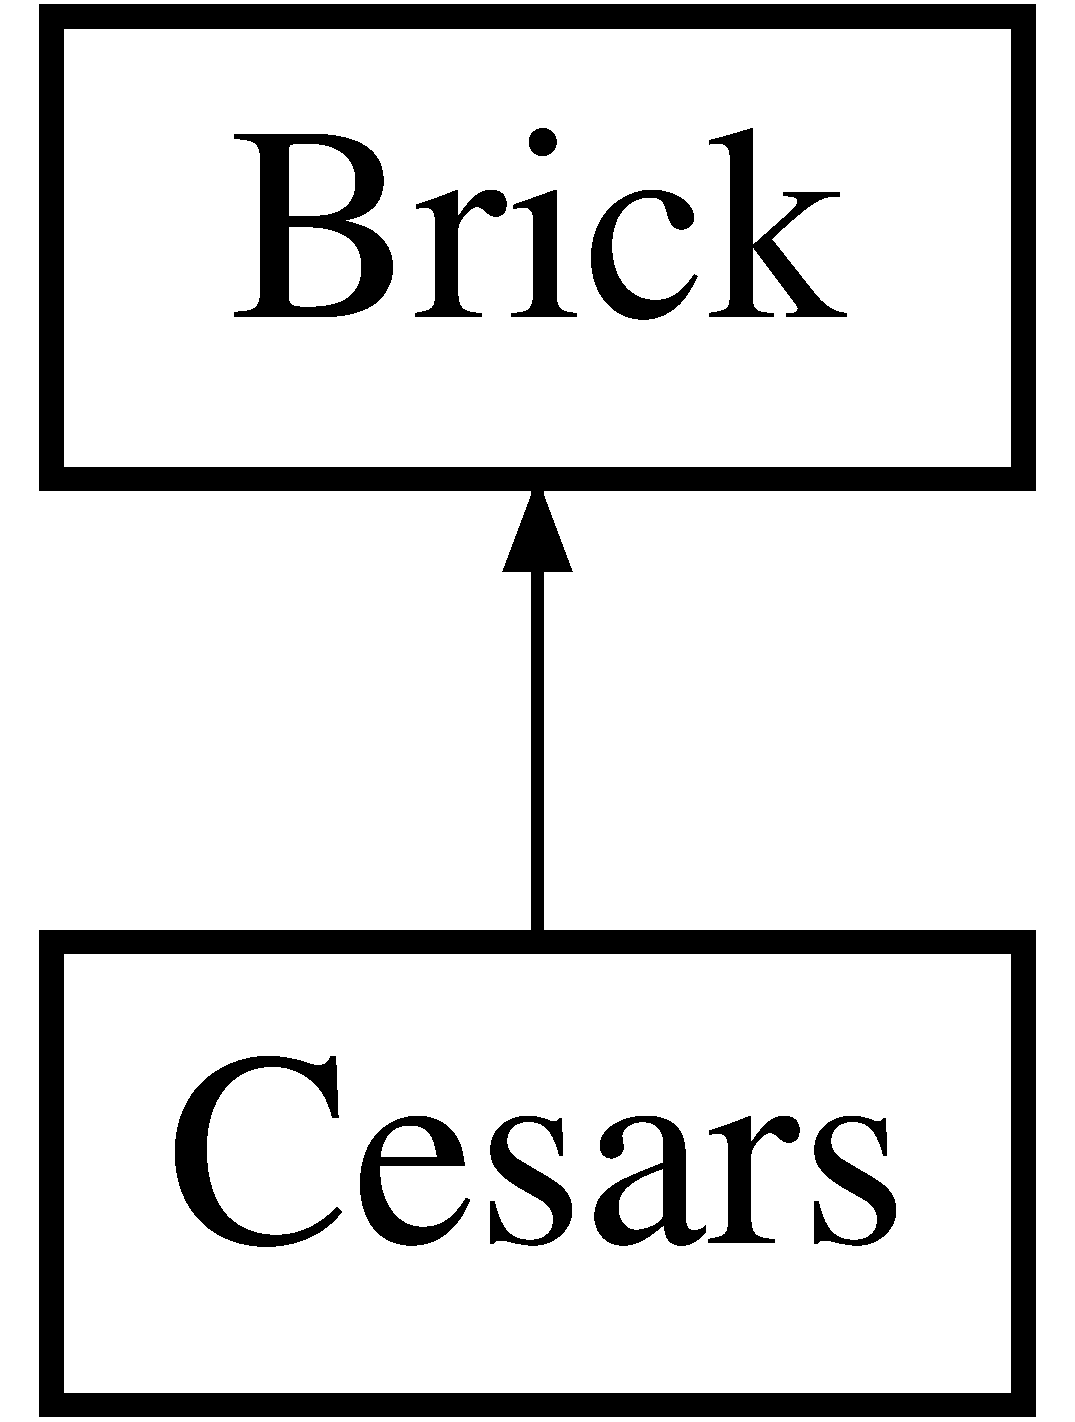
\includegraphics[height=2.000000cm]{dc/dc3/class_cesars}
\end{center}
\end{figure}
\subsection*{Public Member Functions}
\begin{DoxyCompactItemize}
\item 
\hyperlink{class_cesars_ae1fd313aee7d4fc2e2d11cd38167c1d0}{Cesars} ()
\item 
\hyperlink{class_cesars_a23bc7dd430ac18950a25b2a7b2aa7a0a}{$\sim$\+Cesars} ()
\item 
void \hyperlink{class_cesars_aaea2ab4fe1a9eacb640352e0a2d4b422}{present} ()
\item 
void \hyperlink{class_cesars_a8b5bcf3d698a1e11c9e398a61d3a46fc}{get\+\_\+key} ()
\item 
\hyperlink{class_brick_af32354a4d8d1275db35660a96a2cfa3e}{Brick\+::identity} \hyperlink{class_cesars_a4bec14795caf7d1accc9312b04f57eca}{who} ()
\item 
void \hyperlink{class_cesars_a6f8403b49ea1315b95f831e52c22b3f6}{get\+\_\+lib} (int lib)
\item 
\hyperlink{_cesars_8hpp_a7b741beb5ba8737e6aaf6cb5417b9124}{Check\+\_\+\+Cesars} \hyperlink{class_cesars_a9ee84151de75d556612964ca5a88b690}{key\+\_\+check} (int key)
\item 
std\+::string \hyperlink{class_cesars_a0b166b0f93c0949e9f3422e8f6604baa}{chiffre} (std\+::string \&input)
\item 
std\+::string \hyperlink{class_cesars_a9375601dc5baac952212a5125a862a06}{dechiffre} (std\+::string \&input)
\end{DoxyCompactItemize}
\subsection*{Private Attributes}
\begin{DoxyCompactItemize}
\item 
int \hyperlink{class_cesars_a7068dbb885cd0ea992de9c6288e53619}{\+\_\+key}
\end{DoxyCompactItemize}
\subsection*{Additional Inherited Members}


\subsection{Constructor \& Destructor Documentation}
\hypertarget{class_cesars_ae1fd313aee7d4fc2e2d11cd38167c1d0}{}\index{Cesars@{Cesars}!Cesars@{Cesars}}
\index{Cesars@{Cesars}!Cesars@{Cesars}}
\subsubsection[{Cesars()}]{\setlength{\rightskip}{0pt plus 5cm}Cesars\+::\+Cesars (
\begin{DoxyParamCaption}
{}
\end{DoxyParamCaption}
)}\label{class_cesars_ae1fd313aee7d4fc2e2d11cd38167c1d0}
\hypertarget{class_cesars_a23bc7dd430ac18950a25b2a7b2aa7a0a}{}\index{Cesars@{Cesars}!````~Cesars@{$\sim$\+Cesars}}
\index{````~Cesars@{$\sim$\+Cesars}!Cesars@{Cesars}}
\subsubsection[{$\sim$\+Cesars()}]{\setlength{\rightskip}{0pt plus 5cm}Cesars\+::$\sim$\+Cesars (
\begin{DoxyParamCaption}
{}
\end{DoxyParamCaption}
)}\label{class_cesars_a23bc7dd430ac18950a25b2a7b2aa7a0a}


\subsection{Member Function Documentation}
\hypertarget{class_cesars_a0b166b0f93c0949e9f3422e8f6604baa}{}\index{Cesars@{Cesars}!chiffre@{chiffre}}
\index{chiffre@{chiffre}!Cesars@{Cesars}}
\subsubsection[{chiffre(std\+::string \&input)}]{\setlength{\rightskip}{0pt plus 5cm}std\+::string Cesars\+::chiffre (
\begin{DoxyParamCaption}
\item[{std\+::string \&}]{input}
\end{DoxyParamCaption}
)\hspace{0.3cm}{\ttfamily [virtual]}}\label{class_cesars_a0b166b0f93c0949e9f3422e8f6604baa}


Implements \hyperlink{class_brick_a1cddb42fe77c9b6d140004d01ff7ab5b}{Brick}.

\hypertarget{class_cesars_a9375601dc5baac952212a5125a862a06}{}\index{Cesars@{Cesars}!dechiffre@{dechiffre}}
\index{dechiffre@{dechiffre}!Cesars@{Cesars}}
\subsubsection[{dechiffre(std\+::string \&input)}]{\setlength{\rightskip}{0pt plus 5cm}std\+::string Cesars\+::dechiffre (
\begin{DoxyParamCaption}
\item[{std\+::string \&}]{input}
\end{DoxyParamCaption}
)\hspace{0.3cm}{\ttfamily [virtual]}}\label{class_cesars_a9375601dc5baac952212a5125a862a06}


Implements \hyperlink{class_brick_afa3a68ba4f4babecadc6dfd05a2d2040}{Brick}.

\hypertarget{class_cesars_a8b5bcf3d698a1e11c9e398a61d3a46fc}{}\index{Cesars@{Cesars}!get\+\_\+key@{get\+\_\+key}}
\index{get\+\_\+key@{get\+\_\+key}!Cesars@{Cesars}}
\subsubsection[{get\+\_\+key()}]{\setlength{\rightskip}{0pt plus 5cm}void Cesars\+::get\+\_\+key (
\begin{DoxyParamCaption}
{}
\end{DoxyParamCaption}
)\hspace{0.3cm}{\ttfamily [virtual]}}\label{class_cesars_a8b5bcf3d698a1e11c9e398a61d3a46fc}


Implements \hyperlink{class_brick_aeec3d78d8d03e207b4154ff06f637bbe}{Brick}.

\hypertarget{class_cesars_a6f8403b49ea1315b95f831e52c22b3f6}{}\index{Cesars@{Cesars}!get\+\_\+lib@{get\+\_\+lib}}
\index{get\+\_\+lib@{get\+\_\+lib}!Cesars@{Cesars}}
\subsubsection[{get\+\_\+lib(int lib)}]{\setlength{\rightskip}{0pt plus 5cm}void Cesars\+::get\+\_\+lib (
\begin{DoxyParamCaption}
\item[{int}]{lib}
\end{DoxyParamCaption}
)}\label{class_cesars_a6f8403b49ea1315b95f831e52c22b3f6}
\hypertarget{class_cesars_a9ee84151de75d556612964ca5a88b690}{}\index{Cesars@{Cesars}!key\+\_\+check@{key\+\_\+check}}
\index{key\+\_\+check@{key\+\_\+check}!Cesars@{Cesars}}
\subsubsection[{key\+\_\+check(int key)}]{\setlength{\rightskip}{0pt plus 5cm}{\bf Check\+\_\+\+Cesars} Cesars\+::key\+\_\+check (
\begin{DoxyParamCaption}
\item[{int}]{key}
\end{DoxyParamCaption}
)}\label{class_cesars_a9ee84151de75d556612964ca5a88b690}
\hypertarget{class_cesars_aaea2ab4fe1a9eacb640352e0a2d4b422}{}\index{Cesars@{Cesars}!present@{present}}
\index{present@{present}!Cesars@{Cesars}}
\subsubsection[{present()}]{\setlength{\rightskip}{0pt plus 5cm}void Cesars\+::present (
\begin{DoxyParamCaption}
{}
\end{DoxyParamCaption}
)\hspace{0.3cm}{\ttfamily [virtual]}}\label{class_cesars_aaea2ab4fe1a9eacb640352e0a2d4b422}


Implements \hyperlink{class_brick_aa1e9b549787dedc030860f8c75482c8c}{Brick}.

\hypertarget{class_cesars_a4bec14795caf7d1accc9312b04f57eca}{}\index{Cesars@{Cesars}!who@{who}}
\index{who@{who}!Cesars@{Cesars}}
\subsubsection[{who()}]{\setlength{\rightskip}{0pt plus 5cm}{\bf Brick\+::identity} Cesars\+::who (
\begin{DoxyParamCaption}
{}
\end{DoxyParamCaption}
)\hspace{0.3cm}{\ttfamily [virtual]}}\label{class_cesars_a4bec14795caf7d1accc9312b04f57eca}


Implements \hyperlink{class_brick_af6ba737fda1fda2d3fba50de23cbaff0}{Brick}.



\subsection{Member Data Documentation}
\hypertarget{class_cesars_a7068dbb885cd0ea992de9c6288e53619}{}\index{Cesars@{Cesars}!\+\_\+key@{\+\_\+key}}
\index{\+\_\+key@{\+\_\+key}!Cesars@{Cesars}}
\subsubsection[{\+\_\+key}]{\setlength{\rightskip}{0pt plus 5cm}int Cesars\+::\+\_\+key\hspace{0.3cm}{\ttfamily [private]}}\label{class_cesars_a7068dbb885cd0ea992de9c6288e53619}


The documentation for this class was generated from the following files\+:\begin{DoxyCompactItemize}
\item 
includes/core/\hyperlink{_cesars_8hpp}{Cesars.\+hpp}\item 
sources/core/bricks/\hyperlink{_cesars_8cpp}{Cesars.\+cpp}\end{DoxyCompactItemize}

\hypertarget{class_choice}{}\section{Choice Class Reference}
\label{class_choice}\index{Choice@{Choice}}


{\ttfamily \#include $<$Choice.\+hpp$>$}

\subsection*{Public Member Functions}
\begin{DoxyCompactItemize}
\item 
int \hyperlink{class_choice_a4e5f3aa4d48e40b009def0a2b7ff1518}{menu\+\_\+choice} (int min, int max)
\item 
\hyperlink{class_choice_a1f63383fdd4201acc44ae3f1c896774b}{Choice} ()
\item 
\hyperlink{class_choice_ac60418c9d38713ccef3cb0dd1f14a083}{$\sim$\+Choice} ()
\end{DoxyCompactItemize}


\subsection{Constructor \& Destructor Documentation}
\hypertarget{class_choice_a1f63383fdd4201acc44ae3f1c896774b}{}\index{Choice@{Choice}!Choice@{Choice}}
\index{Choice@{Choice}!Choice@{Choice}}
\subsubsection[{Choice()}]{\setlength{\rightskip}{0pt plus 5cm}Choice\+::\+Choice (
\begin{DoxyParamCaption}
{}
\end{DoxyParamCaption}
)}\label{class_choice_a1f63383fdd4201acc44ae3f1c896774b}
\hypertarget{class_choice_ac60418c9d38713ccef3cb0dd1f14a083}{}\index{Choice@{Choice}!````~Choice@{$\sim$\+Choice}}
\index{````~Choice@{$\sim$\+Choice}!Choice@{Choice}}
\subsubsection[{$\sim$\+Choice()}]{\setlength{\rightskip}{0pt plus 5cm}Choice\+::$\sim$\+Choice (
\begin{DoxyParamCaption}
{}
\end{DoxyParamCaption}
)}\label{class_choice_ac60418c9d38713ccef3cb0dd1f14a083}


\subsection{Member Function Documentation}
\hypertarget{class_choice_a4e5f3aa4d48e40b009def0a2b7ff1518}{}\index{Choice@{Choice}!menu\+\_\+choice@{menu\+\_\+choice}}
\index{menu\+\_\+choice@{menu\+\_\+choice}!Choice@{Choice}}
\subsubsection[{menu\+\_\+choice(int min, int max)}]{\setlength{\rightskip}{0pt plus 5cm}int Choice\+::menu\+\_\+choice (
\begin{DoxyParamCaption}
\item[{int}]{min, }
\item[{int}]{max}
\end{DoxyParamCaption}
)}\label{class_choice_a4e5f3aa4d48e40b009def0a2b7ff1518}


The documentation for this class was generated from the following files\+:\begin{DoxyCompactItemize}
\item 
includes/term/\hyperlink{_choice_8hpp}{Choice.\+hpp}\item 
sources/core/\hyperlink{_choice_8cpp}{Choice.\+cpp}\end{DoxyCompactItemize}

\hypertarget{class_constructor}{}\section{Constructor Class Reference}
\label{class_constructor}\index{Constructor@{Constructor}}


{\ttfamily \#include $<$Constructor.\+hpp$>$}

\subsection*{Public Member Functions}
\begin{DoxyCompactItemize}
\item 
void \hyperlink{class_constructor_a16340d50e229caed0d47e81fce95c4f8}{empty\+\_\+list} ()
\item 
bool \hyperlink{class_constructor_a3ca288fc4d5810544a9a3f141202ef85}{add\+\_\+to\+\_\+list} (\hyperlink{class_brick}{Brick} $\ast$brk)
\item 
void \hyperlink{class_constructor_acb69aa2f0d5ad0cdd4f37e2b4e288c28}{get\+\_\+keys} ()
\item 
void \hyperlink{class_constructor_a74c8aab139271c296b7f262b3a2043ea}{present} ()
\item 
bool \hyperlink{class_constructor_a2ecbaf8362625b0760b48f25e36aaeb8}{get\+\_\+lib} (int lib)
\item 
bool \hyperlink{class_constructor_a6f1bf00a6307ee4031066a027dbda079}{status} (bool verbose=false)
\item 
std\+::string $\ast$ \hyperlink{class_constructor_a230d769b93b596cc177543937de05589}{chiffre} (std\+::string const \&input, bool check=true)
\item 
std\+::string $\ast$ \hyperlink{class_constructor_ab47a8bcdd1294c9df31a1ba4e36cff6f}{dechiffre} (std\+::string const \&input, bool check=true)
\item 
\hyperlink{class_constructor_acdc7d45fb66d127f7f954fdd683415dc}{Constructor} ()
\item 
\hyperlink{class_constructor_a4ad4d817192fadf79f16b2a4b72d86a9}{$\sim$\+Constructor} ()
\end{DoxyCompactItemize}
\subsection*{Private Member Functions}
\begin{DoxyCompactItemize}
\item 
bool \hyperlink{class_constructor_ad0f9e7362e27e74fbe3e8710ece78450}{confirm\+\_\+lib} ()
\item 
void \hyperlink{class_constructor_ac49e308a44a30c313b61c7bed07e4555}{set\+\_\+lib} ()
\end{DoxyCompactItemize}
\subsection*{Private Attributes}
\begin{DoxyCompactItemize}
\item 
int \hyperlink{class_constructor_a1b077ce7799b93ca152cdde8da3f724e}{\+\_\+lib}
\item 
bool \hyperlink{class_constructor_af59e3f7a517821f74d0bd2d290efc850}{\+\_\+status\+\_\+lib}
\item 
bool \hyperlink{class_constructor_ae6c63a19938b9afbad0e0f981d298bcc}{\+\_\+status\+\_\+keys}
\item 
std\+::vector$<$ \hyperlink{class_brick}{Brick} $\ast$ $>$ \hyperlink{class_constructor_a199cd25a206aba55a0b617e28413d6c8}{\+\_\+list}
\end{DoxyCompactItemize}


\subsection{Constructor \& Destructor Documentation}
\hypertarget{class_constructor_acdc7d45fb66d127f7f954fdd683415dc}{}\index{Constructor@{Constructor}!Constructor@{Constructor}}
\index{Constructor@{Constructor}!Constructor@{Constructor}}
\subsubsection[{Constructor()}]{\setlength{\rightskip}{0pt plus 5cm}Constructor\+::\+Constructor (
\begin{DoxyParamCaption}
{}
\end{DoxyParamCaption}
)}\label{class_constructor_acdc7d45fb66d127f7f954fdd683415dc}
\hypertarget{class_constructor_a4ad4d817192fadf79f16b2a4b72d86a9}{}\index{Constructor@{Constructor}!````~Constructor@{$\sim$\+Constructor}}
\index{````~Constructor@{$\sim$\+Constructor}!Constructor@{Constructor}}
\subsubsection[{$\sim$\+Constructor()}]{\setlength{\rightskip}{0pt plus 5cm}Constructor\+::$\sim$\+Constructor (
\begin{DoxyParamCaption}
{}
\end{DoxyParamCaption}
)}\label{class_constructor_a4ad4d817192fadf79f16b2a4b72d86a9}


\subsection{Member Function Documentation}
\hypertarget{class_constructor_a3ca288fc4d5810544a9a3f141202ef85}{}\index{Constructor@{Constructor}!add\+\_\+to\+\_\+list@{add\+\_\+to\+\_\+list}}
\index{add\+\_\+to\+\_\+list@{add\+\_\+to\+\_\+list}!Constructor@{Constructor}}
\subsubsection[{add\+\_\+to\+\_\+list(\+Brick $\ast$brk)}]{\setlength{\rightskip}{0pt plus 5cm}bool Constructor\+::add\+\_\+to\+\_\+list (
\begin{DoxyParamCaption}
\item[{{\bf Brick} $\ast$}]{brk}
\end{DoxyParamCaption}
)}\label{class_constructor_a3ca288fc4d5810544a9a3f141202ef85}
\hypertarget{class_constructor_a230d769b93b596cc177543937de05589}{}\index{Constructor@{Constructor}!chiffre@{chiffre}}
\index{chiffre@{chiffre}!Constructor@{Constructor}}
\subsubsection[{chiffre(std\+::string const \&input, bool check=true)}]{\setlength{\rightskip}{0pt plus 5cm}std\+::string $\ast$ Constructor\+::chiffre (
\begin{DoxyParamCaption}
\item[{std\+::string const \&}]{input, }
\item[{bool}]{check = {\ttfamily true}}
\end{DoxyParamCaption}
)}\label{class_constructor_a230d769b93b596cc177543937de05589}
\hypertarget{class_constructor_ad0f9e7362e27e74fbe3e8710ece78450}{}\index{Constructor@{Constructor}!confirm\+\_\+lib@{confirm\+\_\+lib}}
\index{confirm\+\_\+lib@{confirm\+\_\+lib}!Constructor@{Constructor}}
\subsubsection[{confirm\+\_\+lib()}]{\setlength{\rightskip}{0pt plus 5cm}bool Constructor\+::confirm\+\_\+lib (
\begin{DoxyParamCaption}
{}
\end{DoxyParamCaption}
)\hspace{0.3cm}{\ttfamily [private]}}\label{class_constructor_ad0f9e7362e27e74fbe3e8710ece78450}
\hypertarget{class_constructor_ab47a8bcdd1294c9df31a1ba4e36cff6f}{}\index{Constructor@{Constructor}!dechiffre@{dechiffre}}
\index{dechiffre@{dechiffre}!Constructor@{Constructor}}
\subsubsection[{dechiffre(std\+::string const \&input, bool check=true)}]{\setlength{\rightskip}{0pt plus 5cm}std\+::string $\ast$ Constructor\+::dechiffre (
\begin{DoxyParamCaption}
\item[{std\+::string const \&}]{input, }
\item[{bool}]{check = {\ttfamily true}}
\end{DoxyParamCaption}
)}\label{class_constructor_ab47a8bcdd1294c9df31a1ba4e36cff6f}
\hypertarget{class_constructor_a16340d50e229caed0d47e81fce95c4f8}{}\index{Constructor@{Constructor}!empty\+\_\+list@{empty\+\_\+list}}
\index{empty\+\_\+list@{empty\+\_\+list}!Constructor@{Constructor}}
\subsubsection[{empty\+\_\+list()}]{\setlength{\rightskip}{0pt plus 5cm}void Constructor\+::empty\+\_\+list (
\begin{DoxyParamCaption}
{}
\end{DoxyParamCaption}
)}\label{class_constructor_a16340d50e229caed0d47e81fce95c4f8}
\hypertarget{class_constructor_acb69aa2f0d5ad0cdd4f37e2b4e288c28}{}\index{Constructor@{Constructor}!get\+\_\+keys@{get\+\_\+keys}}
\index{get\+\_\+keys@{get\+\_\+keys}!Constructor@{Constructor}}
\subsubsection[{get\+\_\+keys()}]{\setlength{\rightskip}{0pt plus 5cm}void Constructor\+::get\+\_\+keys (
\begin{DoxyParamCaption}
{}
\end{DoxyParamCaption}
)}\label{class_constructor_acb69aa2f0d5ad0cdd4f37e2b4e288c28}
\hypertarget{class_constructor_a2ecbaf8362625b0760b48f25e36aaeb8}{}\index{Constructor@{Constructor}!get\+\_\+lib@{get\+\_\+lib}}
\index{get\+\_\+lib@{get\+\_\+lib}!Constructor@{Constructor}}
\subsubsection[{get\+\_\+lib(int lib)}]{\setlength{\rightskip}{0pt plus 5cm}bool Constructor\+::get\+\_\+lib (
\begin{DoxyParamCaption}
\item[{int}]{lib}
\end{DoxyParamCaption}
)}\label{class_constructor_a2ecbaf8362625b0760b48f25e36aaeb8}
\hypertarget{class_constructor_a74c8aab139271c296b7f262b3a2043ea}{}\index{Constructor@{Constructor}!present@{present}}
\index{present@{present}!Constructor@{Constructor}}
\subsubsection[{present()}]{\setlength{\rightskip}{0pt plus 5cm}void Constructor\+::present (
\begin{DoxyParamCaption}
{}
\end{DoxyParamCaption}
)}\label{class_constructor_a74c8aab139271c296b7f262b3a2043ea}
\hypertarget{class_constructor_ac49e308a44a30c313b61c7bed07e4555}{}\index{Constructor@{Constructor}!set\+\_\+lib@{set\+\_\+lib}}
\index{set\+\_\+lib@{set\+\_\+lib}!Constructor@{Constructor}}
\subsubsection[{set\+\_\+lib()}]{\setlength{\rightskip}{0pt plus 5cm}void Constructor\+::set\+\_\+lib (
\begin{DoxyParamCaption}
{}
\end{DoxyParamCaption}
)\hspace{0.3cm}{\ttfamily [private]}}\label{class_constructor_ac49e308a44a30c313b61c7bed07e4555}
\hypertarget{class_constructor_a6f1bf00a6307ee4031066a027dbda079}{}\index{Constructor@{Constructor}!status@{status}}
\index{status@{status}!Constructor@{Constructor}}
\subsubsection[{status(bool verbose=false)}]{\setlength{\rightskip}{0pt plus 5cm}bool Constructor\+::status (
\begin{DoxyParamCaption}
\item[{bool}]{verbose = {\ttfamily false}}
\end{DoxyParamCaption}
)}\label{class_constructor_a6f1bf00a6307ee4031066a027dbda079}


\subsection{Member Data Documentation}
\hypertarget{class_constructor_a1b077ce7799b93ca152cdde8da3f724e}{}\index{Constructor@{Constructor}!\+\_\+lib@{\+\_\+lib}}
\index{\+\_\+lib@{\+\_\+lib}!Constructor@{Constructor}}
\subsubsection[{\+\_\+lib}]{\setlength{\rightskip}{0pt plus 5cm}int Constructor\+::\+\_\+lib\hspace{0.3cm}{\ttfamily [private]}}\label{class_constructor_a1b077ce7799b93ca152cdde8da3f724e}
\hypertarget{class_constructor_a199cd25a206aba55a0b617e28413d6c8}{}\index{Constructor@{Constructor}!\+\_\+list@{\+\_\+list}}
\index{\+\_\+list@{\+\_\+list}!Constructor@{Constructor}}
\subsubsection[{\+\_\+list}]{\setlength{\rightskip}{0pt plus 5cm}std\+::vector$<${\bf Brick} $\ast$$>$ Constructor\+::\+\_\+list\hspace{0.3cm}{\ttfamily [private]}}\label{class_constructor_a199cd25a206aba55a0b617e28413d6c8}
\hypertarget{class_constructor_ae6c63a19938b9afbad0e0f981d298bcc}{}\index{Constructor@{Constructor}!\+\_\+status\+\_\+keys@{\+\_\+status\+\_\+keys}}
\index{\+\_\+status\+\_\+keys@{\+\_\+status\+\_\+keys}!Constructor@{Constructor}}
\subsubsection[{\+\_\+status\+\_\+keys}]{\setlength{\rightskip}{0pt plus 5cm}bool Constructor\+::\+\_\+status\+\_\+keys\hspace{0.3cm}{\ttfamily [private]}}\label{class_constructor_ae6c63a19938b9afbad0e0f981d298bcc}
\hypertarget{class_constructor_af59e3f7a517821f74d0bd2d290efc850}{}\index{Constructor@{Constructor}!\+\_\+status\+\_\+lib@{\+\_\+status\+\_\+lib}}
\index{\+\_\+status\+\_\+lib@{\+\_\+status\+\_\+lib}!Constructor@{Constructor}}
\subsubsection[{\+\_\+status\+\_\+lib}]{\setlength{\rightskip}{0pt plus 5cm}bool Constructor\+::\+\_\+status\+\_\+lib\hspace{0.3cm}{\ttfamily [private]}}\label{class_constructor_af59e3f7a517821f74d0bd2d290efc850}


The documentation for this class was generated from the following files\+:\begin{DoxyCompactItemize}
\item 
includes/core/\hyperlink{_constructor_8hpp}{Constructor.\+hpp}\item 
sources/core/\+Constructor/\hyperlink{_constructor_8cpp}{Constructor.\+cpp}\item 
sources/core/\+Constructor/\hyperlink{_constructor__lib_8cpp}{Constructor\+\_\+lib.\+cpp}\item 
sources/core/\+Constructor/\hyperlink{_constructor__status_8cpp}{Constructor\+\_\+status.\+cpp}\end{DoxyCompactItemize}

\hypertarget{class_vigenere}{}\section{Vigenere Class Reference}
\label{class_vigenere}\index{Vigenere@{Vigenere}}


{\ttfamily \#include $<$Vigenere.\+hpp$>$}

Inheritance diagram for Vigenere\+:\begin{figure}[H]
\begin{center}
\leavevmode
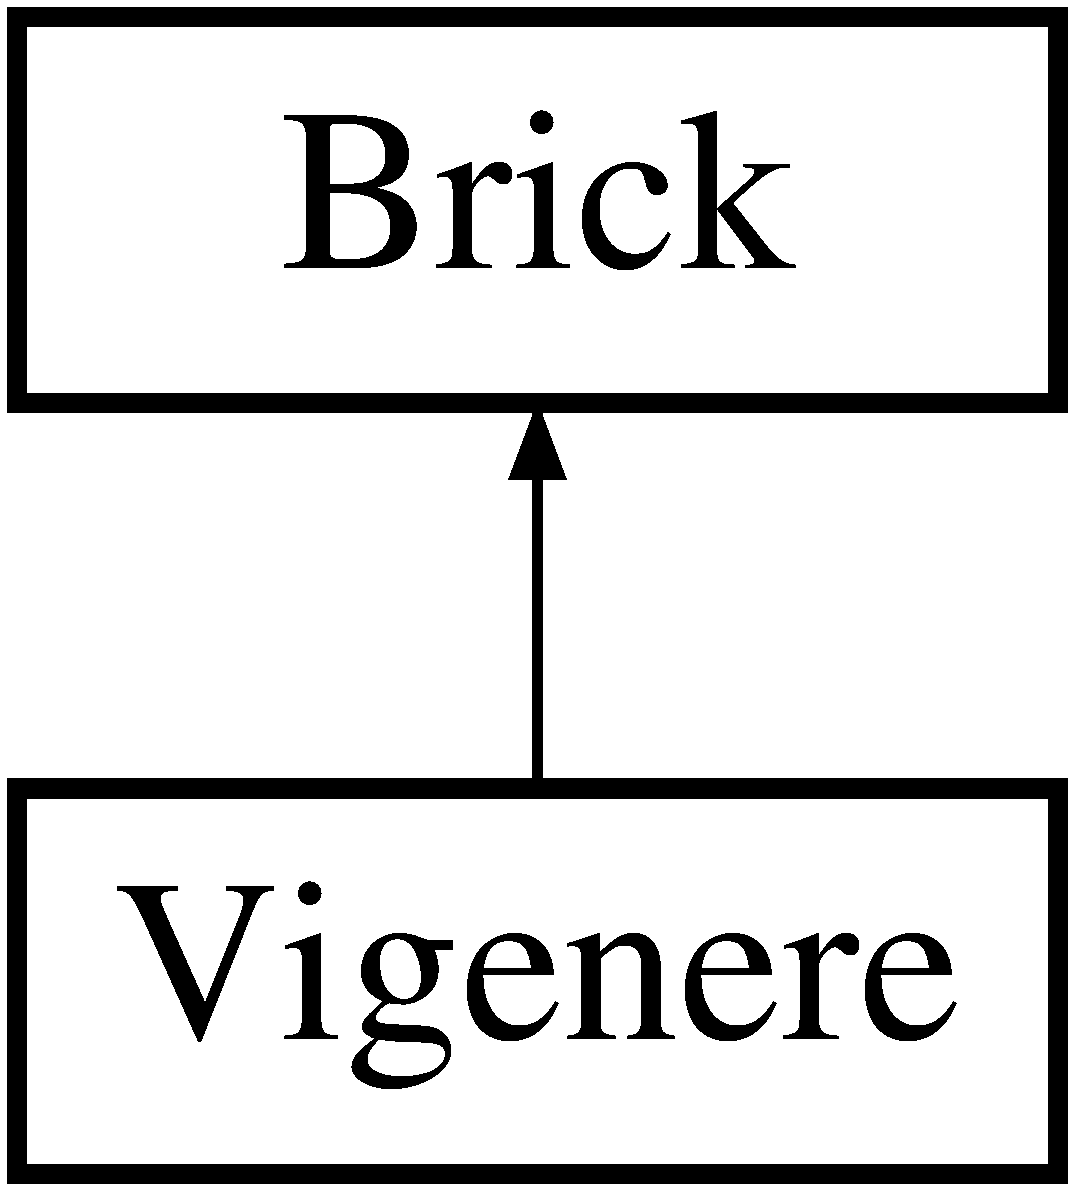
\includegraphics[height=2.000000cm]{d2/dcd/class_vigenere}
\end{center}
\end{figure}
\subsection*{Public Types}
\begin{DoxyCompactItemize}
\item 
enum \hyperlink{class_vigenere_a7c9057eacefc2b70c2f6376808ae24cd}{Check\+\_\+\+Vigenere} \{ \hyperlink{class_vigenere_a7c9057eacefc2b70c2f6376808ae24cda5b266a9ef8e022122a6361ed7b1156d3}{B\+A\+D\+\_\+\+C\+A\+R\+A\+C\+T\+E\+R} = 1, 
\hyperlink{class_vigenere_a7c9057eacefc2b70c2f6376808ae24cdae6a81c51e7f8647713bd2b91e8a64387}{B\+A\+D\+\_\+\+L\+E\+N\+G\+T\+H} = 2, 
\hyperlink{class_vigenere_a7c9057eacefc2b70c2f6376808ae24cda935938c6d3644eff451b497495b99c20}{B\+A\+D\+\_\+\+S\+T\+R\+E\+N\+G\+T\+H} = 3, 
\hyperlink{class_vigenere_a7c9057eacefc2b70c2f6376808ae24cdaaaffac21a07163d0cbaad88a80e98ab7}{G\+O\+O\+D} = 4
 \}
\end{DoxyCompactItemize}
\subsection*{Public Member Functions}
\begin{DoxyCompactItemize}
\item 
\hyperlink{class_vigenere_a7caf4a6411b74aaed0383f479bcf3c69}{Vigenere} ()
\item 
\hyperlink{class_vigenere_a63987a17306659d0ad5f19ac25b95018}{$\sim$\+Vigenere} ()
\item 
void \hyperlink{class_vigenere_a51e5903d16e669efbd738e4554ec9a13}{present} ()
\item 
void \hyperlink{class_vigenere_ac598d07e328e8b633348a0bab923321a}{get\+\_\+key} ()
\item 
char \hyperlink{class_vigenere_aabf8d436dc97f32534fd7901d92ac4b7}{error\+\_\+c} ()
\item 
\hyperlink{class_brick_af32354a4d8d1275db35660a96a2cfa3e}{Brick\+::identity} \hyperlink{class_vigenere_a79338a4aa2e9cea19e06b14103917288}{who} ()
\item 
\hyperlink{class_vigenere_a7c9057eacefc2b70c2f6376808ae24cd}{Check\+\_\+\+Vigenere} \hyperlink{class_vigenere_ad9f7e190fd51729c37d490c90b285c54}{v\+\_\+set\+\_\+key} (std\+::string \&key)
\item 
std\+::string \hyperlink{class_vigenere_a32b9c62addb46ad28e0dec30a4c0cd57}{chiffre} (std\+::string \&input)
\item 
std\+::string \hyperlink{class_vigenere_aeca94f50deaf6416654ea99d5c1156ed}{dechiffre} (std\+::string \&input)
\end{DoxyCompactItemize}
\subsection*{Private Attributes}
\begin{DoxyCompactItemize}
\item 
std\+::string \hyperlink{class_vigenere_af3de7bc9397a9355b64f538572c718de}{\+\_\+key}
\item 
char \hyperlink{class_vigenere_a230349bb11f185853ffb589503368122}{\+\_\+carac\+\_\+error}
\end{DoxyCompactItemize}
\subsection*{Additional Inherited Members}


\subsection{Member Enumeration Documentation}
\hypertarget{class_vigenere_a7c9057eacefc2b70c2f6376808ae24cd}{}\index{Vigenere@{Vigenere}!Check\+\_\+\+Vigenere@{Check\+\_\+\+Vigenere}}
\index{Check\+\_\+\+Vigenere@{Check\+\_\+\+Vigenere}!Vigenere@{Vigenere}}
\subsubsection[{Check\+\_\+\+Vigenere}]{\setlength{\rightskip}{0pt plus 5cm}enum {\bf Vigenere\+::\+Check\+\_\+\+Vigenere}}\label{class_vigenere_a7c9057eacefc2b70c2f6376808ae24cd}
\begin{Desc}
\item[Enumerator]\par
\begin{description}
\index{B\+A\+D\+\_\+\+C\+A\+R\+A\+C\+T\+E\+R@{B\+A\+D\+\_\+\+C\+A\+R\+A\+C\+T\+E\+R}!Vigenere@{Vigenere}}\index{Vigenere@{Vigenere}!B\+A\+D\+\_\+\+C\+A\+R\+A\+C\+T\+E\+R@{B\+A\+D\+\_\+\+C\+A\+R\+A\+C\+T\+E\+R}}\item[{\em 
\hypertarget{class_vigenere_a7c9057eacefc2b70c2f6376808ae24cda5b266a9ef8e022122a6361ed7b1156d3}{}B\+A\+D\+\_\+\+C\+A\+R\+A\+C\+T\+E\+R\label{class_vigenere_a7c9057eacefc2b70c2f6376808ae24cda5b266a9ef8e022122a6361ed7b1156d3}
}]\index{B\+A\+D\+\_\+\+L\+E\+N\+G\+T\+H@{B\+A\+D\+\_\+\+L\+E\+N\+G\+T\+H}!Vigenere@{Vigenere}}\index{Vigenere@{Vigenere}!B\+A\+D\+\_\+\+L\+E\+N\+G\+T\+H@{B\+A\+D\+\_\+\+L\+E\+N\+G\+T\+H}}\item[{\em 
\hypertarget{class_vigenere_a7c9057eacefc2b70c2f6376808ae24cdae6a81c51e7f8647713bd2b91e8a64387}{}B\+A\+D\+\_\+\+L\+E\+N\+G\+T\+H\label{class_vigenere_a7c9057eacefc2b70c2f6376808ae24cdae6a81c51e7f8647713bd2b91e8a64387}
}]\index{B\+A\+D\+\_\+\+S\+T\+R\+E\+N\+G\+T\+H@{B\+A\+D\+\_\+\+S\+T\+R\+E\+N\+G\+T\+H}!Vigenere@{Vigenere}}\index{Vigenere@{Vigenere}!B\+A\+D\+\_\+\+S\+T\+R\+E\+N\+G\+T\+H@{B\+A\+D\+\_\+\+S\+T\+R\+E\+N\+G\+T\+H}}\item[{\em 
\hypertarget{class_vigenere_a7c9057eacefc2b70c2f6376808ae24cda935938c6d3644eff451b497495b99c20}{}B\+A\+D\+\_\+\+S\+T\+R\+E\+N\+G\+T\+H\label{class_vigenere_a7c9057eacefc2b70c2f6376808ae24cda935938c6d3644eff451b497495b99c20}
}]\index{G\+O\+O\+D@{G\+O\+O\+D}!Vigenere@{Vigenere}}\index{Vigenere@{Vigenere}!G\+O\+O\+D@{G\+O\+O\+D}}\item[{\em 
\hypertarget{class_vigenere_a7c9057eacefc2b70c2f6376808ae24cdaaaffac21a07163d0cbaad88a80e98ab7}{}G\+O\+O\+D\label{class_vigenere_a7c9057eacefc2b70c2f6376808ae24cdaaaffac21a07163d0cbaad88a80e98ab7}
}]\end{description}
\end{Desc}


\subsection{Constructor \& Destructor Documentation}
\hypertarget{class_vigenere_a7caf4a6411b74aaed0383f479bcf3c69}{}\index{Vigenere@{Vigenere}!Vigenere@{Vigenere}}
\index{Vigenere@{Vigenere}!Vigenere@{Vigenere}}
\subsubsection[{Vigenere()}]{\setlength{\rightskip}{0pt plus 5cm}Vigenere\+::\+Vigenere (
\begin{DoxyParamCaption}
{}
\end{DoxyParamCaption}
)}\label{class_vigenere_a7caf4a6411b74aaed0383f479bcf3c69}
\hypertarget{class_vigenere_a63987a17306659d0ad5f19ac25b95018}{}\index{Vigenere@{Vigenere}!````~Vigenere@{$\sim$\+Vigenere}}
\index{````~Vigenere@{$\sim$\+Vigenere}!Vigenere@{Vigenere}}
\subsubsection[{$\sim$\+Vigenere()}]{\setlength{\rightskip}{0pt plus 5cm}Vigenere\+::$\sim$\+Vigenere (
\begin{DoxyParamCaption}
{}
\end{DoxyParamCaption}
)}\label{class_vigenere_a63987a17306659d0ad5f19ac25b95018}


\subsection{Member Function Documentation}
\hypertarget{class_vigenere_a32b9c62addb46ad28e0dec30a4c0cd57}{}\index{Vigenere@{Vigenere}!chiffre@{chiffre}}
\index{chiffre@{chiffre}!Vigenere@{Vigenere}}
\subsubsection[{chiffre(std\+::string \&input)}]{\setlength{\rightskip}{0pt plus 5cm}std\+::string Vigenere\+::chiffre (
\begin{DoxyParamCaption}
\item[{std\+::string \&}]{input}
\end{DoxyParamCaption}
)\hspace{0.3cm}{\ttfamily [virtual]}}\label{class_vigenere_a32b9c62addb46ad28e0dec30a4c0cd57}


Implements \hyperlink{class_brick_a1cddb42fe77c9b6d140004d01ff7ab5b}{Brick}.

\hypertarget{class_vigenere_aeca94f50deaf6416654ea99d5c1156ed}{}\index{Vigenere@{Vigenere}!dechiffre@{dechiffre}}
\index{dechiffre@{dechiffre}!Vigenere@{Vigenere}}
\subsubsection[{dechiffre(std\+::string \&input)}]{\setlength{\rightskip}{0pt plus 5cm}std\+::string Vigenere\+::dechiffre (
\begin{DoxyParamCaption}
\item[{std\+::string \&}]{input}
\end{DoxyParamCaption}
)\hspace{0.3cm}{\ttfamily [virtual]}}\label{class_vigenere_aeca94f50deaf6416654ea99d5c1156ed}


Implements \hyperlink{class_brick_afa3a68ba4f4babecadc6dfd05a2d2040}{Brick}.

\hypertarget{class_vigenere_aabf8d436dc97f32534fd7901d92ac4b7}{}\index{Vigenere@{Vigenere}!error\+\_\+c@{error\+\_\+c}}
\index{error\+\_\+c@{error\+\_\+c}!Vigenere@{Vigenere}}
\subsubsection[{error\+\_\+c()}]{\setlength{\rightskip}{0pt plus 5cm}char Vigenere\+::error\+\_\+c (
\begin{DoxyParamCaption}
{}
\end{DoxyParamCaption}
)}\label{class_vigenere_aabf8d436dc97f32534fd7901d92ac4b7}
\hypertarget{class_vigenere_ac598d07e328e8b633348a0bab923321a}{}\index{Vigenere@{Vigenere}!get\+\_\+key@{get\+\_\+key}}
\index{get\+\_\+key@{get\+\_\+key}!Vigenere@{Vigenere}}
\subsubsection[{get\+\_\+key()}]{\setlength{\rightskip}{0pt plus 5cm}void Vigenere\+::get\+\_\+key (
\begin{DoxyParamCaption}
{}
\end{DoxyParamCaption}
)\hspace{0.3cm}{\ttfamily [virtual]}}\label{class_vigenere_ac598d07e328e8b633348a0bab923321a}


Implements \hyperlink{class_brick_aeec3d78d8d03e207b4154ff06f637bbe}{Brick}.

\hypertarget{class_vigenere_a51e5903d16e669efbd738e4554ec9a13}{}\index{Vigenere@{Vigenere}!present@{present}}
\index{present@{present}!Vigenere@{Vigenere}}
\subsubsection[{present()}]{\setlength{\rightskip}{0pt plus 5cm}void Vigenere\+::present (
\begin{DoxyParamCaption}
{}
\end{DoxyParamCaption}
)\hspace{0.3cm}{\ttfamily [virtual]}}\label{class_vigenere_a51e5903d16e669efbd738e4554ec9a13}


Implements \hyperlink{class_brick_aa1e9b549787dedc030860f8c75482c8c}{Brick}.

\hypertarget{class_vigenere_ad9f7e190fd51729c37d490c90b285c54}{}\index{Vigenere@{Vigenere}!v\+\_\+set\+\_\+key@{v\+\_\+set\+\_\+key}}
\index{v\+\_\+set\+\_\+key@{v\+\_\+set\+\_\+key}!Vigenere@{Vigenere}}
\subsubsection[{v\+\_\+set\+\_\+key(std\+::string \&key)}]{\setlength{\rightskip}{0pt plus 5cm}{\bf Vigenere\+::\+Check\+\_\+\+Vigenere} Vigenere\+::v\+\_\+set\+\_\+key (
\begin{DoxyParamCaption}
\item[{std\+::string \&}]{key}
\end{DoxyParamCaption}
)}\label{class_vigenere_ad9f7e190fd51729c37d490c90b285c54}
\hypertarget{class_vigenere_a79338a4aa2e9cea19e06b14103917288}{}\index{Vigenere@{Vigenere}!who@{who}}
\index{who@{who}!Vigenere@{Vigenere}}
\subsubsection[{who()}]{\setlength{\rightskip}{0pt plus 5cm}{\bf Brick\+::identity} Vigenere\+::who (
\begin{DoxyParamCaption}
{}
\end{DoxyParamCaption}
)\hspace{0.3cm}{\ttfamily [virtual]}}\label{class_vigenere_a79338a4aa2e9cea19e06b14103917288}


Implements \hyperlink{class_brick_af6ba737fda1fda2d3fba50de23cbaff0}{Brick}.



\subsection{Member Data Documentation}
\hypertarget{class_vigenere_a230349bb11f185853ffb589503368122}{}\index{Vigenere@{Vigenere}!\+\_\+carac\+\_\+error@{\+\_\+carac\+\_\+error}}
\index{\+\_\+carac\+\_\+error@{\+\_\+carac\+\_\+error}!Vigenere@{Vigenere}}
\subsubsection[{\+\_\+carac\+\_\+error}]{\setlength{\rightskip}{0pt plus 5cm}char Vigenere\+::\+\_\+carac\+\_\+error\hspace{0.3cm}{\ttfamily [private]}}\label{class_vigenere_a230349bb11f185853ffb589503368122}
\hypertarget{class_vigenere_af3de7bc9397a9355b64f538572c718de}{}\index{Vigenere@{Vigenere}!\+\_\+key@{\+\_\+key}}
\index{\+\_\+key@{\+\_\+key}!Vigenere@{Vigenere}}
\subsubsection[{\+\_\+key}]{\setlength{\rightskip}{0pt plus 5cm}std\+::string Vigenere\+::\+\_\+key\hspace{0.3cm}{\ttfamily [private]}}\label{class_vigenere_af3de7bc9397a9355b64f538572c718de}


The documentation for this class was generated from the following files\+:\begin{DoxyCompactItemize}
\item 
includes/core/\hyperlink{_vigenere_8hpp}{Vigenere.\+hpp}\item 
sources/core/bricks/\hyperlink{_vigenere_8cpp}{Vigenere.\+cpp}\end{DoxyCompactItemize}

\chapter{File Documentation}
\hypertarget{102_8hpp}{}\section{includes/core/102.hpp File Reference}
\label{102_8hpp}\index{includes/core/102.\+hpp@{includes/core/102.\+hpp}}
{\ttfamily \#include $<$string$>$}\\*
{\ttfamily \#include $<$Eigen/\+Dense$>$}\\*
{\ttfamily \#include \char`\"{}Brick.\+hpp\char`\"{}}\\*
\subsection*{Classes}
\begin{DoxyCompactItemize}
\item 
class \hyperlink{class__102}{\+\_\+102}
\end{DoxyCompactItemize}

\hypertarget{_brick_8hpp}{}\section{includes/core/\+Brick.hpp File Reference}
\label{_brick_8hpp}\index{includes/core/\+Brick.\+hpp@{includes/core/\+Brick.\+hpp}}
{\ttfamily \#include $<$string$>$}\\*
\subsection*{Classes}
\begin{DoxyCompactItemize}
\item 
class \hyperlink{class_brick}{Brick}
\end{DoxyCompactItemize}

\hypertarget{_cesars_8hpp}{}\section{includes/core/\+Cesars.hpp File Reference}
\label{_cesars_8hpp}\index{includes/core/\+Cesars.\+hpp@{includes/core/\+Cesars.\+hpp}}
{\ttfamily \#include $<$sstream$>$}\\*
{\ttfamily \#include \char`\"{}Brick.\+hpp\char`\"{}}\\*
\subsection*{Classes}
\begin{DoxyCompactItemize}
\item 
class \hyperlink{class_cesars}{Cesars}
\end{DoxyCompactItemize}
\subsection*{Enumerations}
\begin{DoxyCompactItemize}
\item 
enum \hyperlink{_cesars_8hpp_a7b741beb5ba8737e6aaf6cb5417b9124}{Check\+\_\+\+Cesars} \{ \hyperlink{_cesars_8hpp_a7b741beb5ba8737e6aaf6cb5417b9124a788a30dc693d329d8ea028a8400e1618}{B\+A\+D\+\_\+\+V\+A\+L\+U\+E} = 1, 
\hyperlink{_cesars_8hpp_a7b741beb5ba8737e6aaf6cb5417b9124abbc0d1c4bdbb9ef08db3aca00fc00c8b}{B\+A\+D\+\_\+\+M\+O\+D\+U\+L\+O} = 2, 
\hyperlink{_cesars_8hpp_a7b741beb5ba8737e6aaf6cb5417b9124a8eb0135a04a7e7daf1ca4abf2c87832c}{G\+O\+O\+D} = 3
 \}
\end{DoxyCompactItemize}


\subsection{Enumeration Type Documentation}
\hypertarget{_cesars_8hpp_a7b741beb5ba8737e6aaf6cb5417b9124}{}\index{Cesars.\+hpp@{Cesars.\+hpp}!Check\+\_\+\+Cesars@{Check\+\_\+\+Cesars}}
\index{Check\+\_\+\+Cesars@{Check\+\_\+\+Cesars}!Cesars.\+hpp@{Cesars.\+hpp}}
\subsubsection[{Check\+\_\+\+Cesars}]{\setlength{\rightskip}{0pt plus 5cm}enum {\bf Check\+\_\+\+Cesars}}\label{_cesars_8hpp_a7b741beb5ba8737e6aaf6cb5417b9124}
\begin{Desc}
\item[Enumerator]\par
\begin{description}
\index{B\+A\+D\+\_\+\+V\+A\+L\+U\+E@{B\+A\+D\+\_\+\+V\+A\+L\+U\+E}!Cesars.\+hpp@{Cesars.\+hpp}}\index{Cesars.\+hpp@{Cesars.\+hpp}!B\+A\+D\+\_\+\+V\+A\+L\+U\+E@{B\+A\+D\+\_\+\+V\+A\+L\+U\+E}}\item[{\em 
\hypertarget{_cesars_8hpp_a7b741beb5ba8737e6aaf6cb5417b9124a788a30dc693d329d8ea028a8400e1618}{}B\+A\+D\+\_\+\+V\+A\+L\+U\+E\label{_cesars_8hpp_a7b741beb5ba8737e6aaf6cb5417b9124a788a30dc693d329d8ea028a8400e1618}
}]\index{B\+A\+D\+\_\+\+M\+O\+D\+U\+L\+O@{B\+A\+D\+\_\+\+M\+O\+D\+U\+L\+O}!Cesars.\+hpp@{Cesars.\+hpp}}\index{Cesars.\+hpp@{Cesars.\+hpp}!B\+A\+D\+\_\+\+M\+O\+D\+U\+L\+O@{B\+A\+D\+\_\+\+M\+O\+D\+U\+L\+O}}\item[{\em 
\hypertarget{_cesars_8hpp_a7b741beb5ba8737e6aaf6cb5417b9124abbc0d1c4bdbb9ef08db3aca00fc00c8b}{}B\+A\+D\+\_\+\+M\+O\+D\+U\+L\+O\label{_cesars_8hpp_a7b741beb5ba8737e6aaf6cb5417b9124abbc0d1c4bdbb9ef08db3aca00fc00c8b}
}]\index{G\+O\+O\+D@{G\+O\+O\+D}!Cesars.\+hpp@{Cesars.\+hpp}}\index{Cesars.\+hpp@{Cesars.\+hpp}!G\+O\+O\+D@{G\+O\+O\+D}}\item[{\em 
\hypertarget{_cesars_8hpp_a7b741beb5ba8737e6aaf6cb5417b9124a8eb0135a04a7e7daf1ca4abf2c87832c}{}G\+O\+O\+D\label{_cesars_8hpp_a7b741beb5ba8737e6aaf6cb5417b9124a8eb0135a04a7e7daf1ca4abf2c87832c}
}]\end{description}
\end{Desc}

\hypertarget{_constructor_8hpp}{}\section{includes/core/\+Constructor.hpp File Reference}
\label{_constructor_8hpp}\index{includes/core/\+Constructor.\+hpp@{includes/core/\+Constructor.\+hpp}}
{\ttfamily \#include $<$vector$>$}\\*
{\ttfamily \#include \char`\"{}Brick.\+hpp\char`\"{}}\\*
\subsection*{Classes}
\begin{DoxyCompactItemize}
\item 
class \hyperlink{class_constructor}{Constructor}
\end{DoxyCompactItemize}

\hypertarget{_vigenere_8hpp}{}\section{includes/core/\+Vigenere.hpp File Reference}
\label{_vigenere_8hpp}\index{includes/core/\+Vigenere.\+hpp@{includes/core/\+Vigenere.\+hpp}}
{\ttfamily \#include $<$string$>$}\\*
{\ttfamily \#include $<$sstream$>$}\\*
{\ttfamily \#include \char`\"{}Brick.\+hpp\char`\"{}}\\*
\subsection*{Classes}
\begin{DoxyCompactItemize}
\item 
class \hyperlink{class_vigenere}{Vigenere}
\end{DoxyCompactItemize}

\hypertarget{my__maths_8h}{}\section{includes/fichiers/my\+\_\+maths.h File Reference}
\label{my__maths_8h}\index{includes/fichiers/my\+\_\+maths.\+h@{includes/fichiers/my\+\_\+maths.\+h}}
{\ttfamily \#include $<$Eigen/\+Dense$>$}\\*
{\ttfamily \#include $<$string$>$}\\*
{\ttfamily \#include $<$sstream$>$}\\*
\subsection*{Functions}
\begin{DoxyCompactItemize}
\item 
int \hyperlink{my__maths_8h_a63e5111e3846f5f57dcc41c77b1bebbd}{my\+\_\+put\+\_\+nbr\+\_\+base} (int nbr, const char $\ast$base)
\item 
int \hyperlink{my__maths_8h_a5233668aa5c865a73841dc1ad9d8783f}{check\+\_\+neg} (const char $\ast$s)
\item 
int \hyperlink{my__maths_8h_ae4aa38e0e6a8fc19d87997eb6ee540a0}{check\+\_\+base} (const char $\ast$base, int n)
\item 
int \hyperlink{my__maths_8h_aa87f1045795a0b211be0cfacd6eaad2a}{my\+\_\+getnbr\+\_\+base} (const char $\ast$str, const char $\ast$base)
\item 
int \hyperlink{my__maths_8h_ac43986faf8cc81a1ee01eecdc9f8f4ea}{my\+\_\+put\+\_\+nbr\+\_\+base} (int nbr, std\+::string \&base)
\item 
void \hyperlink{my__maths_8h_a658a74c97afeb655c84bee4e681799c5}{base\+\_\+to\+\_\+stream} (int nbr, std\+::string \&base, std\+::stringstream \&out)
\item 
int \hyperlink{my__maths_8h_a9fe00789157e16d86f4798cf99acd23b}{check\+\_\+neg} (std\+::string \&s, int mark=0)
\item 
int \hyperlink{my__maths_8h_aa4252627767342ae7bf021f81ff412e4}{check\+\_\+base} (std\+::string \&base, int n)
\item 
int \hyperlink{my__maths_8h_ace5cc941977a5cc2057563219daccecc}{my\+\_\+getnbr\+\_\+base} (std\+::string \&str, std\+::string \&base, int j=0)
\item 
void \hyperlink{my__maths_8h_aa3b5f6552170b8e1b0e8a22091a9d205}{resize\+\_\+matrix} (Matrix\+Xd \&out, int words)
\item 
void \hyperlink{my__maths_8h_a4a601839d0df5569dab45f7e0a78d123}{matrix\+\_\+initialisator} (Matrix\+Xd \&matrix)
\item 
void \hyperlink{my__maths_8h_aed24fed360419da3259beed4a98a9b45}{user\+\_\+input\+\_\+to\+\_\+matrix} (Matrix\+Xd \&out, std\+::string \&input, const char $\ast$lib)
\end{DoxyCompactItemize}


\subsection{Function Documentation}
\hypertarget{my__maths_8h_a658a74c97afeb655c84bee4e681799c5}{}\index{my\+\_\+maths.\+h@{my\+\_\+maths.\+h}!base\+\_\+to\+\_\+stream@{base\+\_\+to\+\_\+stream}}
\index{base\+\_\+to\+\_\+stream@{base\+\_\+to\+\_\+stream}!my\+\_\+maths.\+h@{my\+\_\+maths.\+h}}
\subsubsection[{base\+\_\+to\+\_\+stream(int nbr, std\+::string \&base, std\+::stringstream \&out)}]{\setlength{\rightskip}{0pt plus 5cm}void base\+\_\+to\+\_\+stream (
\begin{DoxyParamCaption}
\item[{int}]{nbr, }
\item[{std\+::string \&}]{base, }
\item[{std\+::stringstream \&}]{out}
\end{DoxyParamCaption}
)}\label{my__maths_8h_a658a74c97afeb655c84bee4e681799c5}
\hypertarget{my__maths_8h_ae4aa38e0e6a8fc19d87997eb6ee540a0}{}\index{my\+\_\+maths.\+h@{my\+\_\+maths.\+h}!check\+\_\+base@{check\+\_\+base}}
\index{check\+\_\+base@{check\+\_\+base}!my\+\_\+maths.\+h@{my\+\_\+maths.\+h}}
\subsubsection[{check\+\_\+base(const char $\ast$base, int n)}]{\setlength{\rightskip}{0pt plus 5cm}int check\+\_\+base (
\begin{DoxyParamCaption}
\item[{const char $\ast$}]{base, }
\item[{int}]{n}
\end{DoxyParamCaption}
)}\label{my__maths_8h_ae4aa38e0e6a8fc19d87997eb6ee540a0}
\hypertarget{my__maths_8h_aa4252627767342ae7bf021f81ff412e4}{}\index{my\+\_\+maths.\+h@{my\+\_\+maths.\+h}!check\+\_\+base@{check\+\_\+base}}
\index{check\+\_\+base@{check\+\_\+base}!my\+\_\+maths.\+h@{my\+\_\+maths.\+h}}
\subsubsection[{check\+\_\+base(std\+::string \&base, int n)}]{\setlength{\rightskip}{0pt plus 5cm}int check\+\_\+base (
\begin{DoxyParamCaption}
\item[{std\+::string \&}]{base, }
\item[{int}]{n}
\end{DoxyParamCaption}
)}\label{my__maths_8h_aa4252627767342ae7bf021f81ff412e4}
\hypertarget{my__maths_8h_a5233668aa5c865a73841dc1ad9d8783f}{}\index{my\+\_\+maths.\+h@{my\+\_\+maths.\+h}!check\+\_\+neg@{check\+\_\+neg}}
\index{check\+\_\+neg@{check\+\_\+neg}!my\+\_\+maths.\+h@{my\+\_\+maths.\+h}}
\subsubsection[{check\+\_\+neg(const char $\ast$s)}]{\setlength{\rightskip}{0pt plus 5cm}int check\+\_\+neg (
\begin{DoxyParamCaption}
\item[{const char $\ast$}]{s}
\end{DoxyParamCaption}
)}\label{my__maths_8h_a5233668aa5c865a73841dc1ad9d8783f}
\hypertarget{my__maths_8h_a9fe00789157e16d86f4798cf99acd23b}{}\index{my\+\_\+maths.\+h@{my\+\_\+maths.\+h}!check\+\_\+neg@{check\+\_\+neg}}
\index{check\+\_\+neg@{check\+\_\+neg}!my\+\_\+maths.\+h@{my\+\_\+maths.\+h}}
\subsubsection[{check\+\_\+neg(std\+::string \&s, int mark=0)}]{\setlength{\rightskip}{0pt plus 5cm}int check\+\_\+neg (
\begin{DoxyParamCaption}
\item[{std\+::string \&}]{s, }
\item[{int}]{mark = {\ttfamily 0}}
\end{DoxyParamCaption}
)}\label{my__maths_8h_a9fe00789157e16d86f4798cf99acd23b}
\hypertarget{my__maths_8h_a4a601839d0df5569dab45f7e0a78d123}{}\index{my\+\_\+maths.\+h@{my\+\_\+maths.\+h}!matrix\+\_\+initialisator@{matrix\+\_\+initialisator}}
\index{matrix\+\_\+initialisator@{matrix\+\_\+initialisator}!my\+\_\+maths.\+h@{my\+\_\+maths.\+h}}
\subsubsection[{matrix\+\_\+initialisator(\+Matrix\+Xd \&matrix)}]{\setlength{\rightskip}{0pt plus 5cm}void matrix\+\_\+initialisator (
\begin{DoxyParamCaption}
\item[{Matrix\+Xd \&}]{matrix}
\end{DoxyParamCaption}
)}\label{my__maths_8h_a4a601839d0df5569dab45f7e0a78d123}
\hypertarget{my__maths_8h_aa87f1045795a0b211be0cfacd6eaad2a}{}\index{my\+\_\+maths.\+h@{my\+\_\+maths.\+h}!my\+\_\+getnbr\+\_\+base@{my\+\_\+getnbr\+\_\+base}}
\index{my\+\_\+getnbr\+\_\+base@{my\+\_\+getnbr\+\_\+base}!my\+\_\+maths.\+h@{my\+\_\+maths.\+h}}
\subsubsection[{my\+\_\+getnbr\+\_\+base(const char $\ast$str, const char $\ast$base)}]{\setlength{\rightskip}{0pt plus 5cm}int my\+\_\+getnbr\+\_\+base (
\begin{DoxyParamCaption}
\item[{const char $\ast$}]{str, }
\item[{const char $\ast$}]{base}
\end{DoxyParamCaption}
)}\label{my__maths_8h_aa87f1045795a0b211be0cfacd6eaad2a}
\hypertarget{my__maths_8h_ace5cc941977a5cc2057563219daccecc}{}\index{my\+\_\+maths.\+h@{my\+\_\+maths.\+h}!my\+\_\+getnbr\+\_\+base@{my\+\_\+getnbr\+\_\+base}}
\index{my\+\_\+getnbr\+\_\+base@{my\+\_\+getnbr\+\_\+base}!my\+\_\+maths.\+h@{my\+\_\+maths.\+h}}
\subsubsection[{my\+\_\+getnbr\+\_\+base(std\+::string \&str, std\+::string \&base, int j=0)}]{\setlength{\rightskip}{0pt plus 5cm}int my\+\_\+getnbr\+\_\+base (
\begin{DoxyParamCaption}
\item[{std\+::string \&}]{str, }
\item[{std\+::string \&}]{base, }
\item[{int}]{j = {\ttfamily 0}}
\end{DoxyParamCaption}
)}\label{my__maths_8h_ace5cc941977a5cc2057563219daccecc}
\hypertarget{my__maths_8h_a63e5111e3846f5f57dcc41c77b1bebbd}{}\index{my\+\_\+maths.\+h@{my\+\_\+maths.\+h}!my\+\_\+put\+\_\+nbr\+\_\+base@{my\+\_\+put\+\_\+nbr\+\_\+base}}
\index{my\+\_\+put\+\_\+nbr\+\_\+base@{my\+\_\+put\+\_\+nbr\+\_\+base}!my\+\_\+maths.\+h@{my\+\_\+maths.\+h}}
\subsubsection[{my\+\_\+put\+\_\+nbr\+\_\+base(int nbr, const char $\ast$base)}]{\setlength{\rightskip}{0pt plus 5cm}int my\+\_\+put\+\_\+nbr\+\_\+base (
\begin{DoxyParamCaption}
\item[{int}]{nbr, }
\item[{const char $\ast$}]{base}
\end{DoxyParamCaption}
)}\label{my__maths_8h_a63e5111e3846f5f57dcc41c77b1bebbd}
\hypertarget{my__maths_8h_ac43986faf8cc81a1ee01eecdc9f8f4ea}{}\index{my\+\_\+maths.\+h@{my\+\_\+maths.\+h}!my\+\_\+put\+\_\+nbr\+\_\+base@{my\+\_\+put\+\_\+nbr\+\_\+base}}
\index{my\+\_\+put\+\_\+nbr\+\_\+base@{my\+\_\+put\+\_\+nbr\+\_\+base}!my\+\_\+maths.\+h@{my\+\_\+maths.\+h}}
\subsubsection[{my\+\_\+put\+\_\+nbr\+\_\+base(int nbr, std\+::string \&base)}]{\setlength{\rightskip}{0pt plus 5cm}int my\+\_\+put\+\_\+nbr\+\_\+base (
\begin{DoxyParamCaption}
\item[{int}]{nbr, }
\item[{std\+::string \&}]{base}
\end{DoxyParamCaption}
)}\label{my__maths_8h_ac43986faf8cc81a1ee01eecdc9f8f4ea}
\hypertarget{my__maths_8h_aa3b5f6552170b8e1b0e8a22091a9d205}{}\index{my\+\_\+maths.\+h@{my\+\_\+maths.\+h}!resize\+\_\+matrix@{resize\+\_\+matrix}}
\index{resize\+\_\+matrix@{resize\+\_\+matrix}!my\+\_\+maths.\+h@{my\+\_\+maths.\+h}}
\subsubsection[{resize\+\_\+matrix(\+Matrix\+Xd \&out, int words)}]{\setlength{\rightskip}{0pt plus 5cm}void resize\+\_\+matrix (
\begin{DoxyParamCaption}
\item[{Matrix\+Xd \&}]{out, }
\item[{int}]{words}
\end{DoxyParamCaption}
)}\label{my__maths_8h_aa3b5f6552170b8e1b0e8a22091a9d205}
\hypertarget{my__maths_8h_aed24fed360419da3259beed4a98a9b45}{}\index{my\+\_\+maths.\+h@{my\+\_\+maths.\+h}!user\+\_\+input\+\_\+to\+\_\+matrix@{user\+\_\+input\+\_\+to\+\_\+matrix}}
\index{user\+\_\+input\+\_\+to\+\_\+matrix@{user\+\_\+input\+\_\+to\+\_\+matrix}!my\+\_\+maths.\+h@{my\+\_\+maths.\+h}}
\subsubsection[{user\+\_\+input\+\_\+to\+\_\+matrix(\+Matrix\+Xd \&out, std\+::string \&input, const char $\ast$lib)}]{\setlength{\rightskip}{0pt plus 5cm}void user\+\_\+input\+\_\+to\+\_\+matrix (
\begin{DoxyParamCaption}
\item[{Matrix\+Xd \&}]{out, }
\item[{std\+::string \&}]{input, }
\item[{const char $\ast$}]{lib}
\end{DoxyParamCaption}
)}\label{my__maths_8h_aed24fed360419da3259beed4a98a9b45}

\hypertarget{utilitaires_8h}{}\section{includes/fichiers/utilitaires.h File Reference}
\label{utilitaires_8h}\index{includes/fichiers/utilitaires.\+h@{includes/fichiers/utilitaires.\+h}}
{\ttfamily \#include $<$string$>$}\\*
\subsection*{Functions}
\begin{DoxyCompactItemize}
\item 
{\footnotesize template$<$typename T $>$ }\\void \hyperlink{utilitaires_8h_a719922cde969c76bb09db1a96d9799d2}{no\+\_\+tabs} (T str)
\item 
{\footnotesize template$<$typename T $>$ }\\int \hyperlink{utilitaires_8h_a1826941a8f071bbd2a7abbb35a0f9c1e}{no\+\_\+spaces\+\_\+duplicates} (T str)
\item 
{\footnotesize template$<$typename T $>$ }\\void \hyperlink{utilitaires_8h_ac9d178d1d8bacd8168bd3b3ed6dac52d}{no\+\_\+space\+\_\+in\+\_\+begining} (T str)
\item 
{\footnotesize template$<$typename T $>$ }\\void \hyperlink{utilitaires_8h_a561eb26de7fff424913ab780d79f4593}{no\+\_\+space\+\_\+in\+\_\+end} (T str)
\item 
{\footnotesize template$<$typename T $>$ }\\void \hyperlink{utilitaires_8h_a00428962741f5c033d1c919a39e8bdbf}{epur\+\_\+str} (T str)
\item 
{\footnotesize template$<$typename T $>$ }\\int \hyperlink{utilitaires_8h_ab31d207c39cd700042c74a00dbbc01a4}{my\+\_\+isin} (char c, T str)
\item 
const char $\ast$ \hyperlink{utilitaires_8h_a09bd7fb95ac86f1aac333064b7fcd3c3}{lib\+\_\+choice} (int lib)
\item 
int \hyperlink{utilitaires_8h_a53983e7d7866227c86474c95c13fb882}{user\+\_\+input} ()
\item 
void \hyperlink{utilitaires_8h_a551518657dc4ff3f4df34ba6ffac5b7c}{user\+\_\+string} (std\+::string \&in)
\item 
{\footnotesize template$<$typename T $>$ }\\void \hyperlink{utilitaires_8h_a3da53a2996f6631771e6c7919c997ee0}{c\+\_\+str} (T str, char color, int thick=0)
\item 
char \hyperlink{utilitaires_8h_a0383eeba313476dea71c8210b72d91ef}{lib\+\_\+char\+\_\+check} (int lib, std\+::string const \&input)
\item 
bool \hyperlink{utilitaires_8h_acec50b4ca9f56b5935c5835fe7a4e6f2}{lib\+\_\+bool\+\_\+check} (int lib, std\+::string const \&input)
\end{DoxyCompactItemize}


\subsection{Function Documentation}
\hypertarget{utilitaires_8h_a3da53a2996f6631771e6c7919c997ee0}{}\index{utilitaires.\+h@{utilitaires.\+h}!c\+\_\+str@{c\+\_\+str}}
\index{c\+\_\+str@{c\+\_\+str}!utilitaires.\+h@{utilitaires.\+h}}
\subsubsection[{c\+\_\+str(\+T str, char color, int thick=0)}]{\setlength{\rightskip}{0pt plus 5cm}template$<$typename T $>$ void c\+\_\+str (
\begin{DoxyParamCaption}
\item[{T}]{str, }
\item[{char}]{color, }
\item[{int}]{thick = {\ttfamily 0}}
\end{DoxyParamCaption}
)}\label{utilitaires_8h_a3da53a2996f6631771e6c7919c997ee0}
\hypertarget{utilitaires_8h_a00428962741f5c033d1c919a39e8bdbf}{}\index{utilitaires.\+h@{utilitaires.\+h}!epur\+\_\+str@{epur\+\_\+str}}
\index{epur\+\_\+str@{epur\+\_\+str}!utilitaires.\+h@{utilitaires.\+h}}
\subsubsection[{epur\+\_\+str(\+T str)}]{\setlength{\rightskip}{0pt plus 5cm}template$<$typename T $>$ void epur\+\_\+str (
\begin{DoxyParamCaption}
\item[{T}]{str}
\end{DoxyParamCaption}
)}\label{utilitaires_8h_a00428962741f5c033d1c919a39e8bdbf}
\hypertarget{utilitaires_8h_acec50b4ca9f56b5935c5835fe7a4e6f2}{}\index{utilitaires.\+h@{utilitaires.\+h}!lib\+\_\+bool\+\_\+check@{lib\+\_\+bool\+\_\+check}}
\index{lib\+\_\+bool\+\_\+check@{lib\+\_\+bool\+\_\+check}!utilitaires.\+h@{utilitaires.\+h}}
\subsubsection[{lib\+\_\+bool\+\_\+check(int lib, std\+::string const \&input)}]{\setlength{\rightskip}{0pt plus 5cm}bool lib\+\_\+bool\+\_\+check (
\begin{DoxyParamCaption}
\item[{int}]{lib, }
\item[{std\+::string const \&}]{input}
\end{DoxyParamCaption}
)}\label{utilitaires_8h_acec50b4ca9f56b5935c5835fe7a4e6f2}
\hypertarget{utilitaires_8h_a0383eeba313476dea71c8210b72d91ef}{}\index{utilitaires.\+h@{utilitaires.\+h}!lib\+\_\+char\+\_\+check@{lib\+\_\+char\+\_\+check}}
\index{lib\+\_\+char\+\_\+check@{lib\+\_\+char\+\_\+check}!utilitaires.\+h@{utilitaires.\+h}}
\subsubsection[{lib\+\_\+char\+\_\+check(int lib, std\+::string const \&input)}]{\setlength{\rightskip}{0pt plus 5cm}char lib\+\_\+char\+\_\+check (
\begin{DoxyParamCaption}
\item[{int}]{lib, }
\item[{std\+::string const \&}]{input}
\end{DoxyParamCaption}
)}\label{utilitaires_8h_a0383eeba313476dea71c8210b72d91ef}
\hypertarget{utilitaires_8h_a09bd7fb95ac86f1aac333064b7fcd3c3}{}\index{utilitaires.\+h@{utilitaires.\+h}!lib\+\_\+choice@{lib\+\_\+choice}}
\index{lib\+\_\+choice@{lib\+\_\+choice}!utilitaires.\+h@{utilitaires.\+h}}
\subsubsection[{lib\+\_\+choice(int lib)}]{\setlength{\rightskip}{0pt plus 5cm}const char$\ast$ lib\+\_\+choice (
\begin{DoxyParamCaption}
\item[{int}]{lib}
\end{DoxyParamCaption}
)}\label{utilitaires_8h_a09bd7fb95ac86f1aac333064b7fcd3c3}
\hypertarget{utilitaires_8h_ab31d207c39cd700042c74a00dbbc01a4}{}\index{utilitaires.\+h@{utilitaires.\+h}!my\+\_\+isin@{my\+\_\+isin}}
\index{my\+\_\+isin@{my\+\_\+isin}!utilitaires.\+h@{utilitaires.\+h}}
\subsubsection[{my\+\_\+isin(char c, T str)}]{\setlength{\rightskip}{0pt plus 5cm}template$<$typename T $>$ int my\+\_\+isin (
\begin{DoxyParamCaption}
\item[{char}]{c, }
\item[{T}]{str}
\end{DoxyParamCaption}
)}\label{utilitaires_8h_ab31d207c39cd700042c74a00dbbc01a4}
\hypertarget{utilitaires_8h_ac9d178d1d8bacd8168bd3b3ed6dac52d}{}\index{utilitaires.\+h@{utilitaires.\+h}!no\+\_\+space\+\_\+in\+\_\+begining@{no\+\_\+space\+\_\+in\+\_\+begining}}
\index{no\+\_\+space\+\_\+in\+\_\+begining@{no\+\_\+space\+\_\+in\+\_\+begining}!utilitaires.\+h@{utilitaires.\+h}}
\subsubsection[{no\+\_\+space\+\_\+in\+\_\+begining(\+T str)}]{\setlength{\rightskip}{0pt plus 5cm}template$<$typename T $>$ void no\+\_\+space\+\_\+in\+\_\+begining (
\begin{DoxyParamCaption}
\item[{T}]{str}
\end{DoxyParamCaption}
)}\label{utilitaires_8h_ac9d178d1d8bacd8168bd3b3ed6dac52d}
\hypertarget{utilitaires_8h_a561eb26de7fff424913ab780d79f4593}{}\index{utilitaires.\+h@{utilitaires.\+h}!no\+\_\+space\+\_\+in\+\_\+end@{no\+\_\+space\+\_\+in\+\_\+end}}
\index{no\+\_\+space\+\_\+in\+\_\+end@{no\+\_\+space\+\_\+in\+\_\+end}!utilitaires.\+h@{utilitaires.\+h}}
\subsubsection[{no\+\_\+space\+\_\+in\+\_\+end(\+T str)}]{\setlength{\rightskip}{0pt plus 5cm}template$<$typename T $>$ void no\+\_\+space\+\_\+in\+\_\+end (
\begin{DoxyParamCaption}
\item[{T}]{str}
\end{DoxyParamCaption}
)}\label{utilitaires_8h_a561eb26de7fff424913ab780d79f4593}
\hypertarget{utilitaires_8h_a1826941a8f071bbd2a7abbb35a0f9c1e}{}\index{utilitaires.\+h@{utilitaires.\+h}!no\+\_\+spaces\+\_\+duplicates@{no\+\_\+spaces\+\_\+duplicates}}
\index{no\+\_\+spaces\+\_\+duplicates@{no\+\_\+spaces\+\_\+duplicates}!utilitaires.\+h@{utilitaires.\+h}}
\subsubsection[{no\+\_\+spaces\+\_\+duplicates(\+T str)}]{\setlength{\rightskip}{0pt plus 5cm}template$<$typename T $>$ int no\+\_\+spaces\+\_\+duplicates (
\begin{DoxyParamCaption}
\item[{T}]{str}
\end{DoxyParamCaption}
)}\label{utilitaires_8h_a1826941a8f071bbd2a7abbb35a0f9c1e}
\hypertarget{utilitaires_8h_a719922cde969c76bb09db1a96d9799d2}{}\index{utilitaires.\+h@{utilitaires.\+h}!no\+\_\+tabs@{no\+\_\+tabs}}
\index{no\+\_\+tabs@{no\+\_\+tabs}!utilitaires.\+h@{utilitaires.\+h}}
\subsubsection[{no\+\_\+tabs(\+T str)}]{\setlength{\rightskip}{0pt plus 5cm}template$<$typename T $>$ void no\+\_\+tabs (
\begin{DoxyParamCaption}
\item[{T}]{str}
\end{DoxyParamCaption}
)}\label{utilitaires_8h_a719922cde969c76bb09db1a96d9799d2}
\hypertarget{utilitaires_8h_a53983e7d7866227c86474c95c13fb882}{}\index{utilitaires.\+h@{utilitaires.\+h}!user\+\_\+input@{user\+\_\+input}}
\index{user\+\_\+input@{user\+\_\+input}!utilitaires.\+h@{utilitaires.\+h}}
\subsubsection[{user\+\_\+input()}]{\setlength{\rightskip}{0pt plus 5cm}int user\+\_\+input (
\begin{DoxyParamCaption}
{}
\end{DoxyParamCaption}
)}\label{utilitaires_8h_a53983e7d7866227c86474c95c13fb882}
\hypertarget{utilitaires_8h_a551518657dc4ff3f4df34ba6ffac5b7c}{}\index{utilitaires.\+h@{utilitaires.\+h}!user\+\_\+string@{user\+\_\+string}}
\index{user\+\_\+string@{user\+\_\+string}!utilitaires.\+h@{utilitaires.\+h}}
\subsubsection[{user\+\_\+string(std\+::string \&in)}]{\setlength{\rightskip}{0pt plus 5cm}void user\+\_\+string (
\begin{DoxyParamCaption}
\item[{std\+::string \&}]{in}
\end{DoxyParamCaption}
)}\label{utilitaires_8h_a551518657dc4ff3f4df34ba6ffac5b7c}

\hypertarget{qt5__prototypes_8h}{}\section{includes/graph/qt5/qt5\+\_\+prototypes.h File Reference}
\label{qt5__prototypes_8h}\index{includes/graph/qt5/qt5\+\_\+prototypes.\+h@{includes/graph/qt5/qt5\+\_\+prototypes.\+h}}
\subsection*{Functions}
\begin{DoxyCompactItemize}
\item 
int \hyperlink{qt5__prototypes_8h_acd52202723af92854e32e546cb5dd027}{main\+\_\+qt5} (int ac, char $\ast$$\ast$argv)
\end{DoxyCompactItemize}


\subsection{Function Documentation}
\hypertarget{qt5__prototypes_8h_acd52202723af92854e32e546cb5dd027}{}\index{qt5\+\_\+prototypes.\+h@{qt5\+\_\+prototypes.\+h}!main\+\_\+qt5@{main\+\_\+qt5}}
\index{main\+\_\+qt5@{main\+\_\+qt5}!qt5\+\_\+prototypes.\+h@{qt5\+\_\+prototypes.\+h}}
\subsubsection[{main\+\_\+qt5(int ac, char $\ast$$\ast$argv)}]{\setlength{\rightskip}{0pt plus 5cm}int main\+\_\+qt5 (
\begin{DoxyParamCaption}
\item[{int}]{ac, }
\item[{char $\ast$$\ast$}]{argv}
\end{DoxyParamCaption}
)}\label{qt5__prototypes_8h_acd52202723af92854e32e546cb5dd027}

\hypertarget{sdl__prototypes_8h}{}\section{includes/graph/sdl/sdl\+\_\+prototypes.h File Reference}
\label{sdl__prototypes_8h}\index{includes/graph/sdl/sdl\+\_\+prototypes.\+h@{includes/graph/sdl/sdl\+\_\+prototypes.\+h}}
\subsection*{Functions}
\begin{DoxyCompactItemize}
\item 
int \hyperlink{sdl__prototypes_8h_a8b8bb28dec8e39808efed77cad5cc10c}{main\+\_\+sdl} (int ac, char $\ast$$\ast$argv)
\end{DoxyCompactItemize}


\subsection{Function Documentation}
\hypertarget{sdl__prototypes_8h_a8b8bb28dec8e39808efed77cad5cc10c}{}\index{sdl\+\_\+prototypes.\+h@{sdl\+\_\+prototypes.\+h}!main\+\_\+sdl@{main\+\_\+sdl}}
\index{main\+\_\+sdl@{main\+\_\+sdl}!sdl\+\_\+prototypes.\+h@{sdl\+\_\+prototypes.\+h}}
\subsubsection[{main\+\_\+sdl(int ac, char $\ast$$\ast$argv)}]{\setlength{\rightskip}{0pt plus 5cm}int main\+\_\+sdl (
\begin{DoxyParamCaption}
\item[{int}]{ac, }
\item[{char $\ast$$\ast$}]{argv}
\end{DoxyParamCaption}
)}\label{sdl__prototypes_8h_a8b8bb28dec8e39808efed77cad5cc10c}

\hypertarget{instant__prototypes_8h}{}\section{includes/instant/instant\+\_\+prototypes.h File Reference}
\label{instant__prototypes_8h}\index{includes/instant/instant\+\_\+prototypes.\+h@{includes/instant/instant\+\_\+prototypes.\+h}}
\subsection*{Functions}
\begin{DoxyCompactItemize}
\item 
int \hyperlink{instant__prototypes_8h_ad345292bf2197281ca4bcb06805d4481}{main\+\_\+instant} (int ac, char $\ast$$\ast$argv)
\end{DoxyCompactItemize}


\subsection{Function Documentation}
\hypertarget{instant__prototypes_8h_ad345292bf2197281ca4bcb06805d4481}{}\index{instant\+\_\+prototypes.\+h@{instant\+\_\+prototypes.\+h}!main\+\_\+instant@{main\+\_\+instant}}
\index{main\+\_\+instant@{main\+\_\+instant}!instant\+\_\+prototypes.\+h@{instant\+\_\+prototypes.\+h}}
\subsubsection[{main\+\_\+instant(int ac, char $\ast$$\ast$argv)}]{\setlength{\rightskip}{0pt plus 5cm}int main\+\_\+instant (
\begin{DoxyParamCaption}
\item[{int}]{ac, }
\item[{char $\ast$$\ast$}]{argv}
\end{DoxyParamCaption}
)}\label{instant__prototypes_8h_ad345292bf2197281ca4bcb06805d4481}

\hypertarget{_choice_8hpp}{}\section{includes/term/\+Choice.hpp File Reference}
\label{_choice_8hpp}\index{includes/term/\+Choice.\+hpp@{includes/term/\+Choice.\+hpp}}
{\ttfamily \#include $<$string$>$}\\*
\subsection*{Classes}
\begin{DoxyCompactItemize}
\item 
class \hyperlink{class_choice}{Choice}
\end{DoxyCompactItemize}

\hypertarget{term__prototypes_8h}{}\section{includes/term/term\+\_\+prototypes.h File Reference}
\label{term__prototypes_8h}\index{includes/term/term\+\_\+prototypes.\+h@{includes/term/term\+\_\+prototypes.\+h}}
{\ttfamily \#include $<$string$>$}\\*
{\ttfamily \#include $<$Eigen/\+Dense$>$}\\*
\subsection*{Functions}
\begin{DoxyCompactItemize}
\item 
int \hyperlink{term__prototypes_8h_a8a8b8362f87a0291c9aadfd7f5d9f8f9}{main\+\_\+term} ()
\item 
int \hyperlink{term__prototypes_8h_aea6323f020abbe99696af6125b7d1a71}{E\+\_\+102\+\_\+user\+\_\+choices} ()
\item 
int \hyperlink{term__prototypes_8h_ac1bf3f0ece027c37f587b82439717bff}{E\+\_\+102\+\_\+choices} (int choice)
\item 
int \hyperlink{term__prototypes_8h_ace2939666b493765362bca4667d13bb9}{V\+\_\+102\+\_\+user\+\_\+choices} ()
\item 
void \hyperlink{term__prototypes_8h_a8b2b1dfe54ef548b58685424a8334d73}{V\+\_\+102\+\_\+choices} (int choice)
\item 
int \hyperlink{term__prototypes_8h_a43bc14dbfa8db7287cbc94323acd2338}{cesars\+\_\+choices} (int choice)
\item 
int \hyperlink{term__prototypes_8h_adf7419330b39ae100b4bd08fc3738973}{cesars\+\_\+user\+\_\+choices} ()
\item 
void \hyperlink{term__prototypes_8h_a6e292bd6ca297df49b0d6a565a0e9efa}{info\+\_\+\+C\+\_\+and\+\_\+\+V} ()
\item 
void \hyperlink{term__prototypes_8h_a28592aaeb6a3521c744533ad411ffdf8}{info\+\_\+102} ()
\item 
void \hyperlink{term__prototypes_8h_a738816f8f2d18a1f0fb6c7c3cb8fe6be}{info\+\_\+v102} ()
\item 
void \hyperlink{term__prototypes_8h_a3c94f43408b558aba3d7a4c9027bf346}{info\+\_\+alpha} ()
\item 
void \hyperlink{term__prototypes_8h_acb7ee4e5a55a9cf8a9171673ad9ba2b5}{display\+\_\+info} ()
\item 
int \hyperlink{term__prototypes_8h_a67d074b513201480a48489b76ae2bb8d}{vigenere\+\_\+choices} (int choice)
\item 
int \hyperlink{term__prototypes_8h_a1dd80cf29dc324425659148490b3756f}{vigenere\+\_\+user\+\_\+choices} ()
\end{DoxyCompactItemize}


\subsection{Function Documentation}
\hypertarget{term__prototypes_8h_a43bc14dbfa8db7287cbc94323acd2338}{}\index{term\+\_\+prototypes.\+h@{term\+\_\+prototypes.\+h}!cesars\+\_\+choices@{cesars\+\_\+choices}}
\index{cesars\+\_\+choices@{cesars\+\_\+choices}!term\+\_\+prototypes.\+h@{term\+\_\+prototypes.\+h}}
\subsubsection[{cesars\+\_\+choices(int choice)}]{\setlength{\rightskip}{0pt plus 5cm}int cesars\+\_\+choices (
\begin{DoxyParamCaption}
\item[{int}]{choice}
\end{DoxyParamCaption}
)}\label{term__prototypes_8h_a43bc14dbfa8db7287cbc94323acd2338}
\hypertarget{term__prototypes_8h_adf7419330b39ae100b4bd08fc3738973}{}\index{term\+\_\+prototypes.\+h@{term\+\_\+prototypes.\+h}!cesars\+\_\+user\+\_\+choices@{cesars\+\_\+user\+\_\+choices}}
\index{cesars\+\_\+user\+\_\+choices@{cesars\+\_\+user\+\_\+choices}!term\+\_\+prototypes.\+h@{term\+\_\+prototypes.\+h}}
\subsubsection[{cesars\+\_\+user\+\_\+choices()}]{\setlength{\rightskip}{0pt plus 5cm}int cesars\+\_\+user\+\_\+choices (
\begin{DoxyParamCaption}
{}
\end{DoxyParamCaption}
)}\label{term__prototypes_8h_adf7419330b39ae100b4bd08fc3738973}
\hypertarget{term__prototypes_8h_acb7ee4e5a55a9cf8a9171673ad9ba2b5}{}\index{term\+\_\+prototypes.\+h@{term\+\_\+prototypes.\+h}!display\+\_\+info@{display\+\_\+info}}
\index{display\+\_\+info@{display\+\_\+info}!term\+\_\+prototypes.\+h@{term\+\_\+prototypes.\+h}}
\subsubsection[{display\+\_\+info()}]{\setlength{\rightskip}{0pt plus 5cm}void display\+\_\+info (
\begin{DoxyParamCaption}
{}
\end{DoxyParamCaption}
)}\label{term__prototypes_8h_acb7ee4e5a55a9cf8a9171673ad9ba2b5}
\hypertarget{term__prototypes_8h_ac1bf3f0ece027c37f587b82439717bff}{}\index{term\+\_\+prototypes.\+h@{term\+\_\+prototypes.\+h}!E\+\_\+102\+\_\+choices@{E\+\_\+102\+\_\+choices}}
\index{E\+\_\+102\+\_\+choices@{E\+\_\+102\+\_\+choices}!term\+\_\+prototypes.\+h@{term\+\_\+prototypes.\+h}}
\subsubsection[{E\+\_\+102\+\_\+choices(int choice)}]{\setlength{\rightskip}{0pt plus 5cm}int E\+\_\+102\+\_\+choices (
\begin{DoxyParamCaption}
\item[{int}]{choice}
\end{DoxyParamCaption}
)}\label{term__prototypes_8h_ac1bf3f0ece027c37f587b82439717bff}
\hypertarget{term__prototypes_8h_aea6323f020abbe99696af6125b7d1a71}{}\index{term\+\_\+prototypes.\+h@{term\+\_\+prototypes.\+h}!E\+\_\+102\+\_\+user\+\_\+choices@{E\+\_\+102\+\_\+user\+\_\+choices}}
\index{E\+\_\+102\+\_\+user\+\_\+choices@{E\+\_\+102\+\_\+user\+\_\+choices}!term\+\_\+prototypes.\+h@{term\+\_\+prototypes.\+h}}
\subsubsection[{E\+\_\+102\+\_\+user\+\_\+choices()}]{\setlength{\rightskip}{0pt plus 5cm}int E\+\_\+102\+\_\+user\+\_\+choices (
\begin{DoxyParamCaption}
{}
\end{DoxyParamCaption}
)}\label{term__prototypes_8h_aea6323f020abbe99696af6125b7d1a71}
\hypertarget{term__prototypes_8h_a28592aaeb6a3521c744533ad411ffdf8}{}\index{term\+\_\+prototypes.\+h@{term\+\_\+prototypes.\+h}!info\+\_\+102@{info\+\_\+102}}
\index{info\+\_\+102@{info\+\_\+102}!term\+\_\+prototypes.\+h@{term\+\_\+prototypes.\+h}}
\subsubsection[{info\+\_\+102()}]{\setlength{\rightskip}{0pt plus 5cm}void info\+\_\+102 (
\begin{DoxyParamCaption}
{}
\end{DoxyParamCaption}
)}\label{term__prototypes_8h_a28592aaeb6a3521c744533ad411ffdf8}
\hypertarget{term__prototypes_8h_a3c94f43408b558aba3d7a4c9027bf346}{}\index{term\+\_\+prototypes.\+h@{term\+\_\+prototypes.\+h}!info\+\_\+alpha@{info\+\_\+alpha}}
\index{info\+\_\+alpha@{info\+\_\+alpha}!term\+\_\+prototypes.\+h@{term\+\_\+prototypes.\+h}}
\subsubsection[{info\+\_\+alpha()}]{\setlength{\rightskip}{0pt plus 5cm}void info\+\_\+alpha (
\begin{DoxyParamCaption}
{}
\end{DoxyParamCaption}
)}\label{term__prototypes_8h_a3c94f43408b558aba3d7a4c9027bf346}
\hypertarget{term__prototypes_8h_a6e292bd6ca297df49b0d6a565a0e9efa}{}\index{term\+\_\+prototypes.\+h@{term\+\_\+prototypes.\+h}!info\+\_\+\+C\+\_\+and\+\_\+\+V@{info\+\_\+\+C\+\_\+and\+\_\+\+V}}
\index{info\+\_\+\+C\+\_\+and\+\_\+\+V@{info\+\_\+\+C\+\_\+and\+\_\+\+V}!term\+\_\+prototypes.\+h@{term\+\_\+prototypes.\+h}}
\subsubsection[{info\+\_\+\+C\+\_\+and\+\_\+\+V()}]{\setlength{\rightskip}{0pt plus 5cm}void info\+\_\+\+C\+\_\+and\+\_\+\+V (
\begin{DoxyParamCaption}
{}
\end{DoxyParamCaption}
)}\label{term__prototypes_8h_a6e292bd6ca297df49b0d6a565a0e9efa}
\hypertarget{term__prototypes_8h_a738816f8f2d18a1f0fb6c7c3cb8fe6be}{}\index{term\+\_\+prototypes.\+h@{term\+\_\+prototypes.\+h}!info\+\_\+v102@{info\+\_\+v102}}
\index{info\+\_\+v102@{info\+\_\+v102}!term\+\_\+prototypes.\+h@{term\+\_\+prototypes.\+h}}
\subsubsection[{info\+\_\+v102()}]{\setlength{\rightskip}{0pt plus 5cm}void info\+\_\+v102 (
\begin{DoxyParamCaption}
{}
\end{DoxyParamCaption}
)}\label{term__prototypes_8h_a738816f8f2d18a1f0fb6c7c3cb8fe6be}
\hypertarget{term__prototypes_8h_a8a8b8362f87a0291c9aadfd7f5d9f8f9}{}\index{term\+\_\+prototypes.\+h@{term\+\_\+prototypes.\+h}!main\+\_\+term@{main\+\_\+term}}
\index{main\+\_\+term@{main\+\_\+term}!term\+\_\+prototypes.\+h@{term\+\_\+prototypes.\+h}}
\subsubsection[{main\+\_\+term()}]{\setlength{\rightskip}{0pt plus 5cm}int main\+\_\+term (
\begin{DoxyParamCaption}
{}
\end{DoxyParamCaption}
)}\label{term__prototypes_8h_a8a8b8362f87a0291c9aadfd7f5d9f8f9}
\hypertarget{term__prototypes_8h_a8b2b1dfe54ef548b58685424a8334d73}{}\index{term\+\_\+prototypes.\+h@{term\+\_\+prototypes.\+h}!V\+\_\+102\+\_\+choices@{V\+\_\+102\+\_\+choices}}
\index{V\+\_\+102\+\_\+choices@{V\+\_\+102\+\_\+choices}!term\+\_\+prototypes.\+h@{term\+\_\+prototypes.\+h}}
\subsubsection[{V\+\_\+102\+\_\+choices(int choice)}]{\setlength{\rightskip}{0pt plus 5cm}void V\+\_\+102\+\_\+choices (
\begin{DoxyParamCaption}
\item[{int}]{choice}
\end{DoxyParamCaption}
)}\label{term__prototypes_8h_a8b2b1dfe54ef548b58685424a8334d73}
\hypertarget{term__prototypes_8h_ace2939666b493765362bca4667d13bb9}{}\index{term\+\_\+prototypes.\+h@{term\+\_\+prototypes.\+h}!V\+\_\+102\+\_\+user\+\_\+choices@{V\+\_\+102\+\_\+user\+\_\+choices}}
\index{V\+\_\+102\+\_\+user\+\_\+choices@{V\+\_\+102\+\_\+user\+\_\+choices}!term\+\_\+prototypes.\+h@{term\+\_\+prototypes.\+h}}
\subsubsection[{V\+\_\+102\+\_\+user\+\_\+choices()}]{\setlength{\rightskip}{0pt plus 5cm}int V\+\_\+102\+\_\+user\+\_\+choices (
\begin{DoxyParamCaption}
{}
\end{DoxyParamCaption}
)}\label{term__prototypes_8h_ace2939666b493765362bca4667d13bb9}
\hypertarget{term__prototypes_8h_a67d074b513201480a48489b76ae2bb8d}{}\index{term\+\_\+prototypes.\+h@{term\+\_\+prototypes.\+h}!vigenere\+\_\+choices@{vigenere\+\_\+choices}}
\index{vigenere\+\_\+choices@{vigenere\+\_\+choices}!term\+\_\+prototypes.\+h@{term\+\_\+prototypes.\+h}}
\subsubsection[{vigenere\+\_\+choices(int choice)}]{\setlength{\rightskip}{0pt plus 5cm}int vigenere\+\_\+choices (
\begin{DoxyParamCaption}
\item[{int}]{choice}
\end{DoxyParamCaption}
)}\label{term__prototypes_8h_a67d074b513201480a48489b76ae2bb8d}
\hypertarget{term__prototypes_8h_a1dd80cf29dc324425659148490b3756f}{}\index{term\+\_\+prototypes.\+h@{term\+\_\+prototypes.\+h}!vigenere\+\_\+user\+\_\+choices@{vigenere\+\_\+user\+\_\+choices}}
\index{vigenere\+\_\+user\+\_\+choices@{vigenere\+\_\+user\+\_\+choices}!term\+\_\+prototypes.\+h@{term\+\_\+prototypes.\+h}}
\subsubsection[{vigenere\+\_\+user\+\_\+choices()}]{\setlength{\rightskip}{0pt plus 5cm}int vigenere\+\_\+user\+\_\+choices (
\begin{DoxyParamCaption}
{}
\end{DoxyParamCaption}
)}\label{term__prototypes_8h_a1dd80cf29dc324425659148490b3756f}

\hypertarget{_brick_8cpp}{}\section{sources/core/\+Brick.cpp File Reference}
\label{_brick_8cpp}\index{sources/core/\+Brick.\+cpp@{sources/core/\+Brick.\+cpp}}
{\ttfamily \#include $<$string.\+h$>$}\\*
{\ttfamily \#include \char`\"{}Brick.\+hpp\char`\"{}}\\*
{\ttfamily \#include \char`\"{}utilitaires.\+h\char`\"{}}\\*

\hypertarget{__102__brick__functions_8cpp}{}\section{sources/core/bricks/102/\+\_\+102\+\_\+brick\+\_\+functions.cpp File Reference}
\label{__102__brick__functions_8cpp}\index{sources/core/bricks/102/\+\_\+102\+\_\+brick\+\_\+functions.\+cpp@{sources/core/bricks/102/\+\_\+102\+\_\+brick\+\_\+functions.\+cpp}}
{\ttfamily \#include $<$iostream$>$}\\*
{\ttfamily \#include \char`\"{}102.\+hpp\char`\"{}}\\*
{\ttfamily \#include \char`\"{}utilitaires.\+h\char`\"{}}\\*

\hypertarget{__102__chiffre__dechiffre_8cpp}{}\section{sources/core/bricks/102/\+\_\+102\+\_\+chiffre\+\_\+dechiffre.cpp File Reference}
\label{__102__chiffre__dechiffre_8cpp}\index{sources/core/bricks/102/\+\_\+102\+\_\+chiffre\+\_\+dechiffre.\+cpp@{sources/core/bricks/102/\+\_\+102\+\_\+chiffre\+\_\+dechiffre.\+cpp}}
{\ttfamily \#include \char`\"{}102.\+hpp\char`\"{}}\\*
{\ttfamily \#include \char`\"{}my\+\_\+maths.\+h\char`\"{}}\\*
{\ttfamily \#include $<$stdlib.\+h$>$}\\*
{\ttfamily \#include $<$iostream$>$}\\*

\hypertarget{__102__input_8cpp}{}\section{sources/core/bricks/102/\+\_\+102\+\_\+input.cpp File Reference}
\label{__102__input_8cpp}\index{sources/core/bricks/102/\+\_\+102\+\_\+input.\+cpp@{sources/core/bricks/102/\+\_\+102\+\_\+input.\+cpp}}
{\ttfamily \#include $<$iostream$>$}\\*
{\ttfamily \#include \char`\"{}102.\+hpp\char`\"{}}\\*
{\ttfamily \#include \char`\"{}my\+\_\+maths.\+h\char`\"{}}\\*
{\ttfamily \#include \char`\"{}utilitaires.\+h\char`\"{}}\\*

\hypertarget{__102__key__input_8cpp}{}\section{sources/core/bricks/102/\+\_\+102\+\_\+key\+\_\+input.cpp File Reference}
\label{__102__key__input_8cpp}\index{sources/core/bricks/102/\+\_\+102\+\_\+key\+\_\+input.\+cpp@{sources/core/bricks/102/\+\_\+102\+\_\+key\+\_\+input.\+cpp}}
{\ttfamily \#include \char`\"{}my\+\_\+maths.\+h\char`\"{}}\\*
{\ttfamily \#include \char`\"{}utilitaires.\+h\char`\"{}}\\*
{\ttfamily \#include \char`\"{}102.\+hpp\char`\"{}}\\*

\hypertarget{__102__matrix__input_8cpp}{}\section{sources/core/bricks/102/\+\_\+102\+\_\+matrix\+\_\+input.cpp File Reference}
\label{__102__matrix__input_8cpp}\index{sources/core/bricks/102/\+\_\+102\+\_\+matrix\+\_\+input.\+cpp@{sources/core/bricks/102/\+\_\+102\+\_\+matrix\+\_\+input.\+cpp}}
{\ttfamily \#include $<$iostream$>$}\\*
{\ttfamily \#include \char`\"{}term\+\_\+prototypes.\+h\char`\"{}}\\*
{\ttfamily \#include \char`\"{}utilitaires.\+h\char`\"{}}\\*
{\ttfamily \#include \char`\"{}102.\+hpp\char`\"{}}\\*

\hypertarget{__102__utilitaires_8cpp}{}\section{sources/core/bricks/102/\+\_\+102\+\_\+utilitaires.cpp File Reference}
\label{__102__utilitaires_8cpp}\index{sources/core/bricks/102/\+\_\+102\+\_\+utilitaires.\+cpp@{sources/core/bricks/102/\+\_\+102\+\_\+utilitaires.\+cpp}}
{\ttfamily \#include $<$iostream$>$}\\*
{\ttfamily \#include \char`\"{}term\+\_\+prototypes.\+h\char`\"{}}\\*
{\ttfamily \#include \char`\"{}utilitaires.\+h\char`\"{}}\\*
{\ttfamily \#include \char`\"{}102.\+hpp\char`\"{}}\\*

\hypertarget{_cesars_8cpp}{}\section{sources/core/bricks/\+Cesars.cpp File Reference}
\label{_cesars_8cpp}\index{sources/core/bricks/\+Cesars.\+cpp@{sources/core/bricks/\+Cesars.\+cpp}}
{\ttfamily \#include $<$string.\+h$>$}\\*
{\ttfamily \#include $<$iostream$>$}\\*
{\ttfamily \#include \char`\"{}Cesars.\+hpp\char`\"{}}\\*
{\ttfamily \#include \char`\"{}utilitaires.\+h\char`\"{}}\\*

\hypertarget{_vigenere_8cpp}{}\section{sources/core/bricks/\+Vigenere.cpp File Reference}
\label{_vigenere_8cpp}\index{sources/core/bricks/\+Vigenere.\+cpp@{sources/core/bricks/\+Vigenere.\+cpp}}
{\ttfamily \#include $<$string.\+h$>$}\\*
{\ttfamily \#include \char`\"{}utilitaires.\+h\char`\"{}}\\*
{\ttfamily \#include \char`\"{}Vigenere.\+hpp\char`\"{}}\\*
{\ttfamily \#include $<$iostream$>$}\\*

\hypertarget{_choice_8cpp}{}\section{sources/core/\+Choice.cpp File Reference}
\label{_choice_8cpp}\index{sources/core/\+Choice.\+cpp@{sources/core/\+Choice.\+cpp}}
{\ttfamily \#include $<$iostream$>$}\\*
{\ttfamily \#include \char`\"{}utilitaires.\+h\char`\"{}}\\*
{\ttfamily \#include \char`\"{}Choice.\+hpp\char`\"{}}\\*

\hypertarget{_constructor_8cpp}{}\section{sources/core/\+Constructor/\+Constructor.cpp File Reference}
\label{_constructor_8cpp}\index{sources/core/\+Constructor/\+Constructor.\+cpp@{sources/core/\+Constructor/\+Constructor.\+cpp}}
{\ttfamily \#include $<$stdlib.\+h$>$}\\*
{\ttfamily \#include \char`\"{}Constructor.\+hpp\char`\"{}}\\*
{\ttfamily \#include \char`\"{}utilitaires.\+h\char`\"{}}\\*

\hypertarget{_constructor__lib_8cpp}{}\section{sources/core/\+Constructor/\+Constructor\+\_\+lib.cpp File Reference}
\label{_constructor__lib_8cpp}\index{sources/core/\+Constructor/\+Constructor\+\_\+lib.\+cpp@{sources/core/\+Constructor/\+Constructor\+\_\+lib.\+cpp}}
{\ttfamily \#include $<$stdlib.\+h$>$}\\*
{\ttfamily \#include \char`\"{}Constructor.\+hpp\char`\"{}}\\*
{\ttfamily \#include \char`\"{}utilitaires.\+h\char`\"{}}\\*

\hypertarget{_constructor__status_8cpp}{}\section{sources/core/\+Constructor/\+Constructor\+\_\+status.cpp File Reference}
\label{_constructor__status_8cpp}\index{sources/core/\+Constructor/\+Constructor\+\_\+status.\+cpp@{sources/core/\+Constructor/\+Constructor\+\_\+status.\+cpp}}
{\ttfamily \#include $<$iostream$>$}\\*
{\ttfamily \#include \char`\"{}Constructor.\+hpp\char`\"{}}\\*

\hypertarget{bases_8cpp}{}\section{sources/core/maths/bases.cpp File Reference}
\label{bases_8cpp}\index{sources/core/maths/bases.\+cpp@{sources/core/maths/bases.\+cpp}}
{\ttfamily \#include $<$iostream$>$}\\*
{\ttfamily \#include \char`\"{}my\+\_\+maths.\+h\char`\"{}}\\*
\subsection*{Functions}
\begin{DoxyCompactItemize}
\item 
int \hyperlink{bases_8cpp_a63e5111e3846f5f57dcc41c77b1bebbd}{my\+\_\+put\+\_\+nbr\+\_\+base} (int nbr, const char $\ast$base)
\item 
int \hyperlink{bases_8cpp_a5233668aa5c865a73841dc1ad9d8783f}{check\+\_\+neg} (const char $\ast$s)
\item 
int \hyperlink{bases_8cpp_ae4aa38e0e6a8fc19d87997eb6ee540a0}{check\+\_\+base} (const char $\ast$base, int n)
\item 
int \hyperlink{bases_8cpp_aa87f1045795a0b211be0cfacd6eaad2a}{my\+\_\+getnbr\+\_\+base} (const char $\ast$str, const char $\ast$base)
\end{DoxyCompactItemize}


\subsection{Function Documentation}
\hypertarget{bases_8cpp_ae4aa38e0e6a8fc19d87997eb6ee540a0}{}\index{bases.\+cpp@{bases.\+cpp}!check\+\_\+base@{check\+\_\+base}}
\index{check\+\_\+base@{check\+\_\+base}!bases.\+cpp@{bases.\+cpp}}
\subsubsection[{check\+\_\+base(const char $\ast$base, int n)}]{\setlength{\rightskip}{0pt plus 5cm}int check\+\_\+base (
\begin{DoxyParamCaption}
\item[{const char $\ast$}]{base, }
\item[{int}]{n}
\end{DoxyParamCaption}
)}\label{bases_8cpp_ae4aa38e0e6a8fc19d87997eb6ee540a0}
\hypertarget{bases_8cpp_a5233668aa5c865a73841dc1ad9d8783f}{}\index{bases.\+cpp@{bases.\+cpp}!check\+\_\+neg@{check\+\_\+neg}}
\index{check\+\_\+neg@{check\+\_\+neg}!bases.\+cpp@{bases.\+cpp}}
\subsubsection[{check\+\_\+neg(const char $\ast$s)}]{\setlength{\rightskip}{0pt plus 5cm}int check\+\_\+neg (
\begin{DoxyParamCaption}
\item[{const char $\ast$}]{s}
\end{DoxyParamCaption}
)}\label{bases_8cpp_a5233668aa5c865a73841dc1ad9d8783f}
\hypertarget{bases_8cpp_aa87f1045795a0b211be0cfacd6eaad2a}{}\index{bases.\+cpp@{bases.\+cpp}!my\+\_\+getnbr\+\_\+base@{my\+\_\+getnbr\+\_\+base}}
\index{my\+\_\+getnbr\+\_\+base@{my\+\_\+getnbr\+\_\+base}!bases.\+cpp@{bases.\+cpp}}
\subsubsection[{my\+\_\+getnbr\+\_\+base(const char $\ast$str, const char $\ast$base)}]{\setlength{\rightskip}{0pt plus 5cm}int my\+\_\+getnbr\+\_\+base (
\begin{DoxyParamCaption}
\item[{const char $\ast$}]{str, }
\item[{const char $\ast$}]{base}
\end{DoxyParamCaption}
)}\label{bases_8cpp_aa87f1045795a0b211be0cfacd6eaad2a}
\hypertarget{bases_8cpp_a63e5111e3846f5f57dcc41c77b1bebbd}{}\index{bases.\+cpp@{bases.\+cpp}!my\+\_\+put\+\_\+nbr\+\_\+base@{my\+\_\+put\+\_\+nbr\+\_\+base}}
\index{my\+\_\+put\+\_\+nbr\+\_\+base@{my\+\_\+put\+\_\+nbr\+\_\+base}!bases.\+cpp@{bases.\+cpp}}
\subsubsection[{my\+\_\+put\+\_\+nbr\+\_\+base(int nbr, const char $\ast$base)}]{\setlength{\rightskip}{0pt plus 5cm}int my\+\_\+put\+\_\+nbr\+\_\+base (
\begin{DoxyParamCaption}
\item[{int}]{nbr, }
\item[{const char $\ast$}]{base}
\end{DoxyParamCaption}
)}\label{bases_8cpp_a63e5111e3846f5f57dcc41c77b1bebbd}

\hypertarget{bases__string_8cpp}{}\section{sources/core/maths/bases\+\_\+string.cpp File Reference}
\label{bases__string_8cpp}\index{sources/core/maths/bases\+\_\+string.\+cpp@{sources/core/maths/bases\+\_\+string.\+cpp}}
{\ttfamily \#include $<$iostream$>$}\\*
{\ttfamily \#include \char`\"{}term\+\_\+prototypes.\+h\char`\"{}}\\*
\subsection*{Functions}
\begin{DoxyCompactItemize}
\item 
int \hyperlink{bases__string_8cpp_ac43986faf8cc81a1ee01eecdc9f8f4ea}{my\+\_\+put\+\_\+nbr\+\_\+base} (int nbr, std\+::string \&base)
\item 
void \hyperlink{bases__string_8cpp_a658a74c97afeb655c84bee4e681799c5}{base\+\_\+to\+\_\+stream} (int nbr, std\+::string \&base, std\+::stringstream \&out)
\item 
int \hyperlink{bases__string_8cpp_a9aa66123914558e386cdcfa15c6a3599}{check\+\_\+neg} (std\+::string \&s, int mark)
\item 
int \hyperlink{bases__string_8cpp_aa4252627767342ae7bf021f81ff412e4}{check\+\_\+base} (std\+::string \&base, int n)
\item 
int \hyperlink{bases__string_8cpp_a1b9284c20058ada9d8cf13ab8edc493a}{my\+\_\+getnbr\+\_\+base} (std\+::string \&str, std\+::string \&base, int mark)
\end{DoxyCompactItemize}


\subsection{Function Documentation}
\hypertarget{bases__string_8cpp_a658a74c97afeb655c84bee4e681799c5}{}\index{bases\+\_\+string.\+cpp@{bases\+\_\+string.\+cpp}!base\+\_\+to\+\_\+stream@{base\+\_\+to\+\_\+stream}}
\index{base\+\_\+to\+\_\+stream@{base\+\_\+to\+\_\+stream}!bases\+\_\+string.\+cpp@{bases\+\_\+string.\+cpp}}
\subsubsection[{base\+\_\+to\+\_\+stream(int nbr, std\+::string \&base, std\+::stringstream \&out)}]{\setlength{\rightskip}{0pt plus 5cm}void base\+\_\+to\+\_\+stream (
\begin{DoxyParamCaption}
\item[{int}]{nbr, }
\item[{std\+::string \&}]{base, }
\item[{std\+::stringstream \&}]{out}
\end{DoxyParamCaption}
)}\label{bases__string_8cpp_a658a74c97afeb655c84bee4e681799c5}
\hypertarget{bases__string_8cpp_aa4252627767342ae7bf021f81ff412e4}{}\index{bases\+\_\+string.\+cpp@{bases\+\_\+string.\+cpp}!check\+\_\+base@{check\+\_\+base}}
\index{check\+\_\+base@{check\+\_\+base}!bases\+\_\+string.\+cpp@{bases\+\_\+string.\+cpp}}
\subsubsection[{check\+\_\+base(std\+::string \&base, int n)}]{\setlength{\rightskip}{0pt plus 5cm}int check\+\_\+base (
\begin{DoxyParamCaption}
\item[{std\+::string \&}]{base, }
\item[{int}]{n}
\end{DoxyParamCaption}
)}\label{bases__string_8cpp_aa4252627767342ae7bf021f81ff412e4}
\hypertarget{bases__string_8cpp_a9aa66123914558e386cdcfa15c6a3599}{}\index{bases\+\_\+string.\+cpp@{bases\+\_\+string.\+cpp}!check\+\_\+neg@{check\+\_\+neg}}
\index{check\+\_\+neg@{check\+\_\+neg}!bases\+\_\+string.\+cpp@{bases\+\_\+string.\+cpp}}
\subsubsection[{check\+\_\+neg(std\+::string \&s, int mark)}]{\setlength{\rightskip}{0pt plus 5cm}int check\+\_\+neg (
\begin{DoxyParamCaption}
\item[{std\+::string \&}]{s, }
\item[{int}]{mark}
\end{DoxyParamCaption}
)}\label{bases__string_8cpp_a9aa66123914558e386cdcfa15c6a3599}
\hypertarget{bases__string_8cpp_a1b9284c20058ada9d8cf13ab8edc493a}{}\index{bases\+\_\+string.\+cpp@{bases\+\_\+string.\+cpp}!my\+\_\+getnbr\+\_\+base@{my\+\_\+getnbr\+\_\+base}}
\index{my\+\_\+getnbr\+\_\+base@{my\+\_\+getnbr\+\_\+base}!bases\+\_\+string.\+cpp@{bases\+\_\+string.\+cpp}}
\subsubsection[{my\+\_\+getnbr\+\_\+base(std\+::string \&str, std\+::string \&base, int mark)}]{\setlength{\rightskip}{0pt plus 5cm}int my\+\_\+getnbr\+\_\+base (
\begin{DoxyParamCaption}
\item[{std\+::string \&}]{str, }
\item[{std\+::string \&}]{base, }
\item[{int}]{mark}
\end{DoxyParamCaption}
)}\label{bases__string_8cpp_a1b9284c20058ada9d8cf13ab8edc493a}
\hypertarget{bases__string_8cpp_ac43986faf8cc81a1ee01eecdc9f8f4ea}{}\index{bases\+\_\+string.\+cpp@{bases\+\_\+string.\+cpp}!my\+\_\+put\+\_\+nbr\+\_\+base@{my\+\_\+put\+\_\+nbr\+\_\+base}}
\index{my\+\_\+put\+\_\+nbr\+\_\+base@{my\+\_\+put\+\_\+nbr\+\_\+base}!bases\+\_\+string.\+cpp@{bases\+\_\+string.\+cpp}}
\subsubsection[{my\+\_\+put\+\_\+nbr\+\_\+base(int nbr, std\+::string \&base)}]{\setlength{\rightskip}{0pt plus 5cm}int my\+\_\+put\+\_\+nbr\+\_\+base (
\begin{DoxyParamCaption}
\item[{int}]{nbr, }
\item[{std\+::string \&}]{base}
\end{DoxyParamCaption}
)}\label{bases__string_8cpp_ac43986faf8cc81a1ee01eecdc9f8f4ea}

\hypertarget{matrix_8cpp}{}\section{sources/core/maths/matrix.cpp File Reference}
\label{matrix_8cpp}\index{sources/core/maths/matrix.\+cpp@{sources/core/maths/matrix.\+cpp}}
{\ttfamily \#include \char`\"{}term\+\_\+prototypes.\+h\char`\"{}}\\*
{\ttfamily \#include \char`\"{}utilitaires.\+h\char`\"{}}\\*
{\ttfamily \#include \char`\"{}my\+\_\+maths.\+h\char`\"{}}\\*
{\ttfamily \#include $<$iostream$>$}\\*
\subsection*{Functions}
\begin{DoxyCompactItemize}
\item 
void \hyperlink{matrix_8cpp_aa3b5f6552170b8e1b0e8a22091a9d205}{resize\+\_\+matrix} (Matrix\+Xd \&out, int words)
\item 
void \hyperlink{matrix_8cpp_a4a601839d0df5569dab45f7e0a78d123}{matrix\+\_\+initialisator} (Matrix\+Xd \&matrix)
\item 
void \hyperlink{matrix_8cpp_aed24fed360419da3259beed4a98a9b45}{user\+\_\+input\+\_\+to\+\_\+matrix} (Matrix\+Xd \&out, std\+::string \&input, const char $\ast$lib)
\end{DoxyCompactItemize}


\subsection{Function Documentation}
\hypertarget{matrix_8cpp_a4a601839d0df5569dab45f7e0a78d123}{}\index{matrix.\+cpp@{matrix.\+cpp}!matrix\+\_\+initialisator@{matrix\+\_\+initialisator}}
\index{matrix\+\_\+initialisator@{matrix\+\_\+initialisator}!matrix.\+cpp@{matrix.\+cpp}}
\subsubsection[{matrix\+\_\+initialisator(\+Matrix\+Xd \&matrix)}]{\setlength{\rightskip}{0pt plus 5cm}void matrix\+\_\+initialisator (
\begin{DoxyParamCaption}
\item[{Matrix\+Xd \&}]{matrix}
\end{DoxyParamCaption}
)}\label{matrix_8cpp_a4a601839d0df5569dab45f7e0a78d123}
\hypertarget{matrix_8cpp_aa3b5f6552170b8e1b0e8a22091a9d205}{}\index{matrix.\+cpp@{matrix.\+cpp}!resize\+\_\+matrix@{resize\+\_\+matrix}}
\index{resize\+\_\+matrix@{resize\+\_\+matrix}!matrix.\+cpp@{matrix.\+cpp}}
\subsubsection[{resize\+\_\+matrix(\+Matrix\+Xd \&out, int words)}]{\setlength{\rightskip}{0pt plus 5cm}void resize\+\_\+matrix (
\begin{DoxyParamCaption}
\item[{Matrix\+Xd \&}]{out, }
\item[{int}]{words}
\end{DoxyParamCaption}
)}\label{matrix_8cpp_aa3b5f6552170b8e1b0e8a22091a9d205}
\hypertarget{matrix_8cpp_aed24fed360419da3259beed4a98a9b45}{}\index{matrix.\+cpp@{matrix.\+cpp}!user\+\_\+input\+\_\+to\+\_\+matrix@{user\+\_\+input\+\_\+to\+\_\+matrix}}
\index{user\+\_\+input\+\_\+to\+\_\+matrix@{user\+\_\+input\+\_\+to\+\_\+matrix}!matrix.\+cpp@{matrix.\+cpp}}
\subsubsection[{user\+\_\+input\+\_\+to\+\_\+matrix(\+Matrix\+Xd \&out, std\+::string \&input, const char $\ast$lib)}]{\setlength{\rightskip}{0pt plus 5cm}void user\+\_\+input\+\_\+to\+\_\+matrix (
\begin{DoxyParamCaption}
\item[{Matrix\+Xd \&}]{out, }
\item[{std\+::string \&}]{input, }
\item[{const char $\ast$}]{lib}
\end{DoxyParamCaption}
)}\label{matrix_8cpp_aed24fed360419da3259beed4a98a9b45}

\hypertarget{color__str_8cpp}{}\section{sources/core/utilitaires/color\+\_\+str.cpp File Reference}
\label{color__str_8cpp}\index{sources/core/utilitaires/color\+\_\+str.\+cpp@{sources/core/utilitaires/color\+\_\+str.\+cpp}}
{\ttfamily \#include $<$iostream$>$}\\*
{\ttfamily \#include \char`\"{}utilitaires.\+h\char`\"{}}\\*
\subsection*{Functions}
\begin{DoxyCompactItemize}
\item 
template void \hyperlink{color__str_8cpp_a9f349ca4d3f5e8c944fd84757c73af0d}{c\+\_\+str$<$ std\+::string \& $>$} (std\+::string \&str, char color, int thick)
\item 
template void \hyperlink{color__str_8cpp_aa2f66db54e242ff523419541b2395326}{c\+\_\+str$<$ char $\ast$ $>$} (char $\ast$str, char color, int thick)
\item 
template void \hyperlink{color__str_8cpp_a7daa9a9f8a9ba50f2ed22a8e316ff64b}{c\+\_\+str$<$ const char $\ast$ $>$} (const char $\ast$str, char color, int thick)
\item 
{\footnotesize template$<$typename T $>$ }\\void \hyperlink{color__str_8cpp_aafbde6b85aa852c7bf12ba28009dd80a}{c\+\_\+str} (T str, char color, int thick)
\end{DoxyCompactItemize}


\subsection{Function Documentation}
\hypertarget{color__str_8cpp_aafbde6b85aa852c7bf12ba28009dd80a}{}\index{color\+\_\+str.\+cpp@{color\+\_\+str.\+cpp}!c\+\_\+str@{c\+\_\+str}}
\index{c\+\_\+str@{c\+\_\+str}!color\+\_\+str.\+cpp@{color\+\_\+str.\+cpp}}
\subsubsection[{c\+\_\+str(\+T str, char color, int thick)}]{\setlength{\rightskip}{0pt plus 5cm}template$<$typename T $>$ void c\+\_\+str (
\begin{DoxyParamCaption}
\item[{T}]{str, }
\item[{char}]{color, }
\item[{int}]{thick}
\end{DoxyParamCaption}
)}\label{color__str_8cpp_aafbde6b85aa852c7bf12ba28009dd80a}
\hypertarget{color__str_8cpp_aa2f66db54e242ff523419541b2395326}{}\index{color\+\_\+str.\+cpp@{color\+\_\+str.\+cpp}!c\+\_\+str$<$ char $\ast$ $>$@{c\+\_\+str$<$ char $\ast$ $>$}}
\index{c\+\_\+str$<$ char $\ast$ $>$@{c\+\_\+str$<$ char $\ast$ $>$}!color\+\_\+str.\+cpp@{color\+\_\+str.\+cpp}}
\subsubsection[{c\+\_\+str$<$ char $\ast$ $>$(char $\ast$str, char color, int thick)}]{\setlength{\rightskip}{0pt plus 5cm}template void {\bf c\+\_\+str}$<$ char $\ast$ $>$ (
\begin{DoxyParamCaption}
\item[{char $\ast$}]{str, }
\item[{char}]{color, }
\item[{int}]{thick}
\end{DoxyParamCaption}
)}\label{color__str_8cpp_aa2f66db54e242ff523419541b2395326}
\hypertarget{color__str_8cpp_a7daa9a9f8a9ba50f2ed22a8e316ff64b}{}\index{color\+\_\+str.\+cpp@{color\+\_\+str.\+cpp}!c\+\_\+str$<$ const char $\ast$ $>$@{c\+\_\+str$<$ const char $\ast$ $>$}}
\index{c\+\_\+str$<$ const char $\ast$ $>$@{c\+\_\+str$<$ const char $\ast$ $>$}!color\+\_\+str.\+cpp@{color\+\_\+str.\+cpp}}
\subsubsection[{c\+\_\+str$<$ const char $\ast$ $>$(const char $\ast$str, char color, int thick)}]{\setlength{\rightskip}{0pt plus 5cm}template void {\bf c\+\_\+str}$<$ const char $\ast$ $>$ (
\begin{DoxyParamCaption}
\item[{const char $\ast$}]{str, }
\item[{char}]{color, }
\item[{int}]{thick}
\end{DoxyParamCaption}
)}\label{color__str_8cpp_a7daa9a9f8a9ba50f2ed22a8e316ff64b}
\hypertarget{color__str_8cpp_a9f349ca4d3f5e8c944fd84757c73af0d}{}\index{color\+\_\+str.\+cpp@{color\+\_\+str.\+cpp}!c\+\_\+str$<$ std\+::string \& $>$@{c\+\_\+str$<$ std\+::string \& $>$}}
\index{c\+\_\+str$<$ std\+::string \& $>$@{c\+\_\+str$<$ std\+::string \& $>$}!color\+\_\+str.\+cpp@{color\+\_\+str.\+cpp}}
\subsubsection[{c\+\_\+str$<$ std\+::string \& $>$(std\+::string \&str, char color, int thick)}]{\setlength{\rightskip}{0pt plus 5cm}template void {\bf c\+\_\+str}$<$ std\+::string \& $>$ (
\begin{DoxyParamCaption}
\item[{std\+::string \&}]{str, }
\item[{char}]{color, }
\item[{int}]{thick}
\end{DoxyParamCaption}
)}\label{color__str_8cpp_a9f349ca4d3f5e8c944fd84757c73af0d}

\hypertarget{epur__str_8cpp}{}\section{sources/core/utilitaires/epur\+\_\+str.cpp File Reference}
\label{epur__str_8cpp}\index{sources/core/utilitaires/epur\+\_\+str.\+cpp@{sources/core/utilitaires/epur\+\_\+str.\+cpp}}
{\ttfamily \#include \char`\"{}utilitaires.\+h\char`\"{}}\\*
\subsection*{Functions}
\begin{DoxyCompactItemize}
\item 
template void \hyperlink{epur__str_8cpp_a67b8505d7d346bb7b2cbe0a24522a41b}{no\+\_\+tabs$<$ char $\ast$ $>$} (char $\ast$str)
\item 
template void \hyperlink{epur__str_8cpp_af3065c893eb8d5759f6cffbc75302616}{no\+\_\+tabs$<$ std\+::string \& $>$} (std\+::string \&str)
\item 
template int \hyperlink{epur__str_8cpp_afb4830eb32d987865d44e7463bec32ac}{no\+\_\+spaces\+\_\+duplicates$<$ char $\ast$ $>$} (char $\ast$str)
\item 
template int \hyperlink{epur__str_8cpp_a89f24c681b03ea22498edb6e98aa49e8}{no\+\_\+spaces\+\_\+duplicates$<$ std\+::string \& $>$} (std\+::string \&str)
\item 
template void \hyperlink{epur__str_8cpp_aab6de84d37d78e0a80d146ef3767a885}{no\+\_\+space\+\_\+in\+\_\+begining$<$ char $\ast$ $>$} (char $\ast$str)
\item 
template void \hyperlink{epur__str_8cpp_ae74e8f55e3704bc55006a3cbfcf795fd}{no\+\_\+space\+\_\+in\+\_\+begining$<$ std\+::string \& $>$} (std\+::string \&str)
\item 
template void \hyperlink{epur__str_8cpp_a774dcd2c17f34aec4df1eb9e4171fec3}{no\+\_\+space\+\_\+in\+\_\+end$<$ char $\ast$ $>$} (char $\ast$str)
\item 
template void \hyperlink{epur__str_8cpp_a91d8fce894e854758aa5588290167e69}{no\+\_\+space\+\_\+in\+\_\+end$<$ std\+::string \& $>$} (std\+::string \&str)
\item 
template void \hyperlink{epur__str_8cpp_a756d405f1e7ab33a04350b1ef26e388c}{epur\+\_\+str$<$ char $\ast$ $>$} (char $\ast$str)
\item 
template void \hyperlink{epur__str_8cpp_ae0f23f6cf60f15d3f6dc264c057286ae}{epur\+\_\+str$<$ std\+::string $>$} (std\+::string str)
\item 
template void \hyperlink{epur__str_8cpp_ae1bc2818ff26839e26f71e0293976fbf}{epur\+\_\+str$<$ std\+::string \& $>$} (std\+::string \&str)
\item 
{\footnotesize template$<$typename T $>$ }\\void \hyperlink{epur__str_8cpp_a719922cde969c76bb09db1a96d9799d2}{no\+\_\+tabs} (T str)
\item 
{\footnotesize template$<$typename T $>$ }\\int \hyperlink{epur__str_8cpp_a1826941a8f071bbd2a7abbb35a0f9c1e}{no\+\_\+spaces\+\_\+duplicates} (T str)
\item 
{\footnotesize template$<$typename T $>$ }\\void \hyperlink{epur__str_8cpp_ac9d178d1d8bacd8168bd3b3ed6dac52d}{no\+\_\+space\+\_\+in\+\_\+begining} (T str)
\item 
{\footnotesize template$<$typename T $>$ }\\void \hyperlink{epur__str_8cpp_a561eb26de7fff424913ab780d79f4593}{no\+\_\+space\+\_\+in\+\_\+end} (T str)
\item 
{\footnotesize template$<$typename T $>$ }\\void \hyperlink{epur__str_8cpp_a00428962741f5c033d1c919a39e8bdbf}{epur\+\_\+str} (T str)
\end{DoxyCompactItemize}


\subsection{Function Documentation}
\hypertarget{epur__str_8cpp_a00428962741f5c033d1c919a39e8bdbf}{}\index{epur\+\_\+str.\+cpp@{epur\+\_\+str.\+cpp}!epur\+\_\+str@{epur\+\_\+str}}
\index{epur\+\_\+str@{epur\+\_\+str}!epur\+\_\+str.\+cpp@{epur\+\_\+str.\+cpp}}
\subsubsection[{epur\+\_\+str(\+T str)}]{\setlength{\rightskip}{0pt plus 5cm}template$<$typename T $>$ void epur\+\_\+str (
\begin{DoxyParamCaption}
\item[{T}]{str}
\end{DoxyParamCaption}
)}\label{epur__str_8cpp_a00428962741f5c033d1c919a39e8bdbf}
\hypertarget{epur__str_8cpp_a756d405f1e7ab33a04350b1ef26e388c}{}\index{epur\+\_\+str.\+cpp@{epur\+\_\+str.\+cpp}!epur\+\_\+str$<$ char $\ast$ $>$@{epur\+\_\+str$<$ char $\ast$ $>$}}
\index{epur\+\_\+str$<$ char $\ast$ $>$@{epur\+\_\+str$<$ char $\ast$ $>$}!epur\+\_\+str.\+cpp@{epur\+\_\+str.\+cpp}}
\subsubsection[{epur\+\_\+str$<$ char $\ast$ $>$(char $\ast$str)}]{\setlength{\rightskip}{0pt plus 5cm}template void {\bf epur\+\_\+str}$<$ char $\ast$ $>$ (
\begin{DoxyParamCaption}
\item[{char $\ast$}]{str}
\end{DoxyParamCaption}
)}\label{epur__str_8cpp_a756d405f1e7ab33a04350b1ef26e388c}
\hypertarget{epur__str_8cpp_ae1bc2818ff26839e26f71e0293976fbf}{}\index{epur\+\_\+str.\+cpp@{epur\+\_\+str.\+cpp}!epur\+\_\+str$<$ std\+::string \& $>$@{epur\+\_\+str$<$ std\+::string \& $>$}}
\index{epur\+\_\+str$<$ std\+::string \& $>$@{epur\+\_\+str$<$ std\+::string \& $>$}!epur\+\_\+str.\+cpp@{epur\+\_\+str.\+cpp}}
\subsubsection[{epur\+\_\+str$<$ std\+::string \& $>$(std\+::string \&str)}]{\setlength{\rightskip}{0pt plus 5cm}template void {\bf epur\+\_\+str}$<$ std\+::string \& $>$ (
\begin{DoxyParamCaption}
\item[{std\+::string \&}]{str}
\end{DoxyParamCaption}
)}\label{epur__str_8cpp_ae1bc2818ff26839e26f71e0293976fbf}
\hypertarget{epur__str_8cpp_ae0f23f6cf60f15d3f6dc264c057286ae}{}\index{epur\+\_\+str.\+cpp@{epur\+\_\+str.\+cpp}!epur\+\_\+str$<$ std\+::string $>$@{epur\+\_\+str$<$ std\+::string $>$}}
\index{epur\+\_\+str$<$ std\+::string $>$@{epur\+\_\+str$<$ std\+::string $>$}!epur\+\_\+str.\+cpp@{epur\+\_\+str.\+cpp}}
\subsubsection[{epur\+\_\+str$<$ std\+::string $>$(std\+::string str)}]{\setlength{\rightskip}{0pt plus 5cm}template void {\bf epur\+\_\+str}$<$ std\+::string $>$ (
\begin{DoxyParamCaption}
\item[{std\+::string}]{str}
\end{DoxyParamCaption}
)}\label{epur__str_8cpp_ae0f23f6cf60f15d3f6dc264c057286ae}
\hypertarget{epur__str_8cpp_ac9d178d1d8bacd8168bd3b3ed6dac52d}{}\index{epur\+\_\+str.\+cpp@{epur\+\_\+str.\+cpp}!no\+\_\+space\+\_\+in\+\_\+begining@{no\+\_\+space\+\_\+in\+\_\+begining}}
\index{no\+\_\+space\+\_\+in\+\_\+begining@{no\+\_\+space\+\_\+in\+\_\+begining}!epur\+\_\+str.\+cpp@{epur\+\_\+str.\+cpp}}
\subsubsection[{no\+\_\+space\+\_\+in\+\_\+begining(\+T str)}]{\setlength{\rightskip}{0pt plus 5cm}template$<$typename T $>$ void no\+\_\+space\+\_\+in\+\_\+begining (
\begin{DoxyParamCaption}
\item[{T}]{str}
\end{DoxyParamCaption}
)}\label{epur__str_8cpp_ac9d178d1d8bacd8168bd3b3ed6dac52d}
\hypertarget{epur__str_8cpp_aab6de84d37d78e0a80d146ef3767a885}{}\index{epur\+\_\+str.\+cpp@{epur\+\_\+str.\+cpp}!no\+\_\+space\+\_\+in\+\_\+begining$<$ char $\ast$ $>$@{no\+\_\+space\+\_\+in\+\_\+begining$<$ char $\ast$ $>$}}
\index{no\+\_\+space\+\_\+in\+\_\+begining$<$ char $\ast$ $>$@{no\+\_\+space\+\_\+in\+\_\+begining$<$ char $\ast$ $>$}!epur\+\_\+str.\+cpp@{epur\+\_\+str.\+cpp}}
\subsubsection[{no\+\_\+space\+\_\+in\+\_\+begining$<$ char $\ast$ $>$(char $\ast$str)}]{\setlength{\rightskip}{0pt plus 5cm}template void {\bf no\+\_\+space\+\_\+in\+\_\+begining}$<$ char $\ast$ $>$ (
\begin{DoxyParamCaption}
\item[{char $\ast$}]{str}
\end{DoxyParamCaption}
)}\label{epur__str_8cpp_aab6de84d37d78e0a80d146ef3767a885}
\hypertarget{epur__str_8cpp_ae74e8f55e3704bc55006a3cbfcf795fd}{}\index{epur\+\_\+str.\+cpp@{epur\+\_\+str.\+cpp}!no\+\_\+space\+\_\+in\+\_\+begining$<$ std\+::string \& $>$@{no\+\_\+space\+\_\+in\+\_\+begining$<$ std\+::string \& $>$}}
\index{no\+\_\+space\+\_\+in\+\_\+begining$<$ std\+::string \& $>$@{no\+\_\+space\+\_\+in\+\_\+begining$<$ std\+::string \& $>$}!epur\+\_\+str.\+cpp@{epur\+\_\+str.\+cpp}}
\subsubsection[{no\+\_\+space\+\_\+in\+\_\+begining$<$ std\+::string \& $>$(std\+::string \&str)}]{\setlength{\rightskip}{0pt plus 5cm}template void {\bf no\+\_\+space\+\_\+in\+\_\+begining}$<$ std\+::string \& $>$ (
\begin{DoxyParamCaption}
\item[{std\+::string \&}]{str}
\end{DoxyParamCaption}
)}\label{epur__str_8cpp_ae74e8f55e3704bc55006a3cbfcf795fd}
\hypertarget{epur__str_8cpp_a561eb26de7fff424913ab780d79f4593}{}\index{epur\+\_\+str.\+cpp@{epur\+\_\+str.\+cpp}!no\+\_\+space\+\_\+in\+\_\+end@{no\+\_\+space\+\_\+in\+\_\+end}}
\index{no\+\_\+space\+\_\+in\+\_\+end@{no\+\_\+space\+\_\+in\+\_\+end}!epur\+\_\+str.\+cpp@{epur\+\_\+str.\+cpp}}
\subsubsection[{no\+\_\+space\+\_\+in\+\_\+end(\+T str)}]{\setlength{\rightskip}{0pt plus 5cm}template$<$typename T $>$ void no\+\_\+space\+\_\+in\+\_\+end (
\begin{DoxyParamCaption}
\item[{T}]{str}
\end{DoxyParamCaption}
)}\label{epur__str_8cpp_a561eb26de7fff424913ab780d79f4593}
\hypertarget{epur__str_8cpp_a774dcd2c17f34aec4df1eb9e4171fec3}{}\index{epur\+\_\+str.\+cpp@{epur\+\_\+str.\+cpp}!no\+\_\+space\+\_\+in\+\_\+end$<$ char $\ast$ $>$@{no\+\_\+space\+\_\+in\+\_\+end$<$ char $\ast$ $>$}}
\index{no\+\_\+space\+\_\+in\+\_\+end$<$ char $\ast$ $>$@{no\+\_\+space\+\_\+in\+\_\+end$<$ char $\ast$ $>$}!epur\+\_\+str.\+cpp@{epur\+\_\+str.\+cpp}}
\subsubsection[{no\+\_\+space\+\_\+in\+\_\+end$<$ char $\ast$ $>$(char $\ast$str)}]{\setlength{\rightskip}{0pt plus 5cm}template void {\bf no\+\_\+space\+\_\+in\+\_\+end}$<$ char $\ast$ $>$ (
\begin{DoxyParamCaption}
\item[{char $\ast$}]{str}
\end{DoxyParamCaption}
)}\label{epur__str_8cpp_a774dcd2c17f34aec4df1eb9e4171fec3}
\hypertarget{epur__str_8cpp_a91d8fce894e854758aa5588290167e69}{}\index{epur\+\_\+str.\+cpp@{epur\+\_\+str.\+cpp}!no\+\_\+space\+\_\+in\+\_\+end$<$ std\+::string \& $>$@{no\+\_\+space\+\_\+in\+\_\+end$<$ std\+::string \& $>$}}
\index{no\+\_\+space\+\_\+in\+\_\+end$<$ std\+::string \& $>$@{no\+\_\+space\+\_\+in\+\_\+end$<$ std\+::string \& $>$}!epur\+\_\+str.\+cpp@{epur\+\_\+str.\+cpp}}
\subsubsection[{no\+\_\+space\+\_\+in\+\_\+end$<$ std\+::string \& $>$(std\+::string \&str)}]{\setlength{\rightskip}{0pt plus 5cm}template void {\bf no\+\_\+space\+\_\+in\+\_\+end}$<$ std\+::string \& $>$ (
\begin{DoxyParamCaption}
\item[{std\+::string \&}]{str}
\end{DoxyParamCaption}
)}\label{epur__str_8cpp_a91d8fce894e854758aa5588290167e69}
\hypertarget{epur__str_8cpp_a1826941a8f071bbd2a7abbb35a0f9c1e}{}\index{epur\+\_\+str.\+cpp@{epur\+\_\+str.\+cpp}!no\+\_\+spaces\+\_\+duplicates@{no\+\_\+spaces\+\_\+duplicates}}
\index{no\+\_\+spaces\+\_\+duplicates@{no\+\_\+spaces\+\_\+duplicates}!epur\+\_\+str.\+cpp@{epur\+\_\+str.\+cpp}}
\subsubsection[{no\+\_\+spaces\+\_\+duplicates(\+T str)}]{\setlength{\rightskip}{0pt plus 5cm}template$<$typename T $>$ int no\+\_\+spaces\+\_\+duplicates (
\begin{DoxyParamCaption}
\item[{T}]{str}
\end{DoxyParamCaption}
)}\label{epur__str_8cpp_a1826941a8f071bbd2a7abbb35a0f9c1e}
\hypertarget{epur__str_8cpp_afb4830eb32d987865d44e7463bec32ac}{}\index{epur\+\_\+str.\+cpp@{epur\+\_\+str.\+cpp}!no\+\_\+spaces\+\_\+duplicates$<$ char $\ast$ $>$@{no\+\_\+spaces\+\_\+duplicates$<$ char $\ast$ $>$}}
\index{no\+\_\+spaces\+\_\+duplicates$<$ char $\ast$ $>$@{no\+\_\+spaces\+\_\+duplicates$<$ char $\ast$ $>$}!epur\+\_\+str.\+cpp@{epur\+\_\+str.\+cpp}}
\subsubsection[{no\+\_\+spaces\+\_\+duplicates$<$ char $\ast$ $>$(char $\ast$str)}]{\setlength{\rightskip}{0pt plus 5cm}template int {\bf no\+\_\+spaces\+\_\+duplicates}$<$ char $\ast$ $>$ (
\begin{DoxyParamCaption}
\item[{char $\ast$}]{str}
\end{DoxyParamCaption}
)}\label{epur__str_8cpp_afb4830eb32d987865d44e7463bec32ac}
\hypertarget{epur__str_8cpp_a89f24c681b03ea22498edb6e98aa49e8}{}\index{epur\+\_\+str.\+cpp@{epur\+\_\+str.\+cpp}!no\+\_\+spaces\+\_\+duplicates$<$ std\+::string \& $>$@{no\+\_\+spaces\+\_\+duplicates$<$ std\+::string \& $>$}}
\index{no\+\_\+spaces\+\_\+duplicates$<$ std\+::string \& $>$@{no\+\_\+spaces\+\_\+duplicates$<$ std\+::string \& $>$}!epur\+\_\+str.\+cpp@{epur\+\_\+str.\+cpp}}
\subsubsection[{no\+\_\+spaces\+\_\+duplicates$<$ std\+::string \& $>$(std\+::string \&str)}]{\setlength{\rightskip}{0pt plus 5cm}template int {\bf no\+\_\+spaces\+\_\+duplicates}$<$ std\+::string \& $>$ (
\begin{DoxyParamCaption}
\item[{std\+::string \&}]{str}
\end{DoxyParamCaption}
)}\label{epur__str_8cpp_a89f24c681b03ea22498edb6e98aa49e8}
\hypertarget{epur__str_8cpp_a719922cde969c76bb09db1a96d9799d2}{}\index{epur\+\_\+str.\+cpp@{epur\+\_\+str.\+cpp}!no\+\_\+tabs@{no\+\_\+tabs}}
\index{no\+\_\+tabs@{no\+\_\+tabs}!epur\+\_\+str.\+cpp@{epur\+\_\+str.\+cpp}}
\subsubsection[{no\+\_\+tabs(\+T str)}]{\setlength{\rightskip}{0pt plus 5cm}template$<$typename T $>$ void no\+\_\+tabs (
\begin{DoxyParamCaption}
\item[{T}]{str}
\end{DoxyParamCaption}
)}\label{epur__str_8cpp_a719922cde969c76bb09db1a96d9799d2}
\hypertarget{epur__str_8cpp_a67b8505d7d346bb7b2cbe0a24522a41b}{}\index{epur\+\_\+str.\+cpp@{epur\+\_\+str.\+cpp}!no\+\_\+tabs$<$ char $\ast$ $>$@{no\+\_\+tabs$<$ char $\ast$ $>$}}
\index{no\+\_\+tabs$<$ char $\ast$ $>$@{no\+\_\+tabs$<$ char $\ast$ $>$}!epur\+\_\+str.\+cpp@{epur\+\_\+str.\+cpp}}
\subsubsection[{no\+\_\+tabs$<$ char $\ast$ $>$(char $\ast$str)}]{\setlength{\rightskip}{0pt plus 5cm}template void {\bf no\+\_\+tabs}$<$ char $\ast$ $>$ (
\begin{DoxyParamCaption}
\item[{char $\ast$}]{str}
\end{DoxyParamCaption}
)}\label{epur__str_8cpp_a67b8505d7d346bb7b2cbe0a24522a41b}
\hypertarget{epur__str_8cpp_af3065c893eb8d5759f6cffbc75302616}{}\index{epur\+\_\+str.\+cpp@{epur\+\_\+str.\+cpp}!no\+\_\+tabs$<$ std\+::string \& $>$@{no\+\_\+tabs$<$ std\+::string \& $>$}}
\index{no\+\_\+tabs$<$ std\+::string \& $>$@{no\+\_\+tabs$<$ std\+::string \& $>$}!epur\+\_\+str.\+cpp@{epur\+\_\+str.\+cpp}}
\subsubsection[{no\+\_\+tabs$<$ std\+::string \& $>$(std\+::string \&str)}]{\setlength{\rightskip}{0pt plus 5cm}template void {\bf no\+\_\+tabs}$<$ std\+::string \& $>$ (
\begin{DoxyParamCaption}
\item[{std\+::string \&}]{str}
\end{DoxyParamCaption}
)}\label{epur__str_8cpp_af3065c893eb8d5759f6cffbc75302616}

\hypertarget{isin_8cpp}{}\section{sources/core/utilitaires/isin.cpp File Reference}
\label{isin_8cpp}\index{sources/core/utilitaires/isin.\+cpp@{sources/core/utilitaires/isin.\+cpp}}
{\ttfamily \#include \char`\"{}utilitaires.\+h\char`\"{}}\\*
\subsection*{Functions}
\begin{DoxyCompactItemize}
\item 
template int \hyperlink{isin_8cpp_a484a1fce9c21a10be32eb2a346540515}{my\+\_\+isin$<$ char $\ast$ $>$} (char c, char $\ast$str)
\item 
template int \hyperlink{isin_8cpp_abbf97e95f63d2de7b419bd38bdd1a113}{my\+\_\+isin$<$ const char $\ast$ $>$} (char c, const char $\ast$str)
\item 
template int \hyperlink{isin_8cpp_a7423aaad25c6c70f238562f95d5e4a33}{my\+\_\+isin$<$ std\+::string \& $>$} (char c, std\+::string \&str)
\item 
template int \hyperlink{isin_8cpp_a6f1801641e7622b180e83eaba2c73c8f}{my\+\_\+isin$<$ const std\+::string \& $>$} (char c, const std\+::string \&str)
\item 
{\footnotesize template$<$typename T $>$ }\\int \hyperlink{isin_8cpp_ab31d207c39cd700042c74a00dbbc01a4}{my\+\_\+isin} (char c, T str)
\end{DoxyCompactItemize}


\subsection{Function Documentation}
\hypertarget{isin_8cpp_ab31d207c39cd700042c74a00dbbc01a4}{}\index{isin.\+cpp@{isin.\+cpp}!my\+\_\+isin@{my\+\_\+isin}}
\index{my\+\_\+isin@{my\+\_\+isin}!isin.\+cpp@{isin.\+cpp}}
\subsubsection[{my\+\_\+isin(char c, T str)}]{\setlength{\rightskip}{0pt plus 5cm}template$<$typename T $>$ int my\+\_\+isin (
\begin{DoxyParamCaption}
\item[{char}]{c, }
\item[{T}]{str}
\end{DoxyParamCaption}
)}\label{isin_8cpp_ab31d207c39cd700042c74a00dbbc01a4}
\hypertarget{isin_8cpp_a484a1fce9c21a10be32eb2a346540515}{}\index{isin.\+cpp@{isin.\+cpp}!my\+\_\+isin$<$ char $\ast$ $>$@{my\+\_\+isin$<$ char $\ast$ $>$}}
\index{my\+\_\+isin$<$ char $\ast$ $>$@{my\+\_\+isin$<$ char $\ast$ $>$}!isin.\+cpp@{isin.\+cpp}}
\subsubsection[{my\+\_\+isin$<$ char $\ast$ $>$(char c, char $\ast$str)}]{\setlength{\rightskip}{0pt plus 5cm}template int {\bf my\+\_\+isin}$<$ char $\ast$ $>$ (
\begin{DoxyParamCaption}
\item[{char}]{c, }
\item[{char $\ast$}]{str}
\end{DoxyParamCaption}
)}\label{isin_8cpp_a484a1fce9c21a10be32eb2a346540515}
\hypertarget{isin_8cpp_abbf97e95f63d2de7b419bd38bdd1a113}{}\index{isin.\+cpp@{isin.\+cpp}!my\+\_\+isin$<$ const char $\ast$ $>$@{my\+\_\+isin$<$ const char $\ast$ $>$}}
\index{my\+\_\+isin$<$ const char $\ast$ $>$@{my\+\_\+isin$<$ const char $\ast$ $>$}!isin.\+cpp@{isin.\+cpp}}
\subsubsection[{my\+\_\+isin$<$ const char $\ast$ $>$(char c, const char $\ast$str)}]{\setlength{\rightskip}{0pt plus 5cm}template int {\bf my\+\_\+isin}$<$ const char $\ast$ $>$ (
\begin{DoxyParamCaption}
\item[{char}]{c, }
\item[{const char $\ast$}]{str}
\end{DoxyParamCaption}
)}\label{isin_8cpp_abbf97e95f63d2de7b419bd38bdd1a113}
\hypertarget{isin_8cpp_a6f1801641e7622b180e83eaba2c73c8f}{}\index{isin.\+cpp@{isin.\+cpp}!my\+\_\+isin$<$ const std\+::string \& $>$@{my\+\_\+isin$<$ const std\+::string \& $>$}}
\index{my\+\_\+isin$<$ const std\+::string \& $>$@{my\+\_\+isin$<$ const std\+::string \& $>$}!isin.\+cpp@{isin.\+cpp}}
\subsubsection[{my\+\_\+isin$<$ const std\+::string \& $>$(char c, const std\+::string \&str)}]{\setlength{\rightskip}{0pt plus 5cm}template int {\bf my\+\_\+isin}$<$ const std\+::string \& $>$ (
\begin{DoxyParamCaption}
\item[{char}]{c, }
\item[{const std\+::string \&}]{str}
\end{DoxyParamCaption}
)}\label{isin_8cpp_a6f1801641e7622b180e83eaba2c73c8f}
\hypertarget{isin_8cpp_a7423aaad25c6c70f238562f95d5e4a33}{}\index{isin.\+cpp@{isin.\+cpp}!my\+\_\+isin$<$ std\+::string \& $>$@{my\+\_\+isin$<$ std\+::string \& $>$}}
\index{my\+\_\+isin$<$ std\+::string \& $>$@{my\+\_\+isin$<$ std\+::string \& $>$}!isin.\+cpp@{isin.\+cpp}}
\subsubsection[{my\+\_\+isin$<$ std\+::string \& $>$(char c, std\+::string \&str)}]{\setlength{\rightskip}{0pt plus 5cm}template int {\bf my\+\_\+isin}$<$ std\+::string \& $>$ (
\begin{DoxyParamCaption}
\item[{char}]{c, }
\item[{std\+::string \&}]{str}
\end{DoxyParamCaption}
)}\label{isin_8cpp_a7423aaad25c6c70f238562f95d5e4a33}

\hypertarget{lib_8cpp}{}\section{sources/core/utilitaires/lib.cpp File Reference}
\label{lib_8cpp}\index{sources/core/utilitaires/lib.\+cpp@{sources/core/utilitaires/lib.\+cpp}}
{\ttfamily \#include $<$iostream$>$}\\*
\subsection*{Functions}
\begin{DoxyCompactItemize}
\item 
const char $\ast$ \hyperlink{lib_8cpp_a09bd7fb95ac86f1aac333064b7fcd3c3}{lib\+\_\+choice} (int lib)
\end{DoxyCompactItemize}


\subsection{Function Documentation}
\hypertarget{lib_8cpp_a09bd7fb95ac86f1aac333064b7fcd3c3}{}\index{lib.\+cpp@{lib.\+cpp}!lib\+\_\+choice@{lib\+\_\+choice}}
\index{lib\+\_\+choice@{lib\+\_\+choice}!lib.\+cpp@{lib.\+cpp}}
\subsubsection[{lib\+\_\+choice(int lib)}]{\setlength{\rightskip}{0pt plus 5cm}const char$\ast$ lib\+\_\+choice (
\begin{DoxyParamCaption}
\item[{int}]{lib}
\end{DoxyParamCaption}
)}\label{lib_8cpp_a09bd7fb95ac86f1aac333064b7fcd3c3}

\hypertarget{lib__check_8cpp}{}\section{sources/core/utilitaires/lib\+\_\+check.cpp File Reference}
\label{lib__check_8cpp}\index{sources/core/utilitaires/lib\+\_\+check.\+cpp@{sources/core/utilitaires/lib\+\_\+check.\+cpp}}
{\ttfamily \#include \char`\"{}utilitaires.\+h\char`\"{}}\\*
\subsection*{Functions}
\begin{DoxyCompactItemize}
\item 
char \hyperlink{lib__check_8cpp_acb4202d78c7de5971ae77a5f33282d56}{lib\+\_\+char\+\_\+check} (int libi, std\+::string const \&input)
\item 
bool \hyperlink{lib__check_8cpp_a8e39e3608e6d9dc362da047bc11eb703}{lib\+\_\+bool\+\_\+check} (int libi, std\+::string const \&input)
\end{DoxyCompactItemize}


\subsection{Function Documentation}
\hypertarget{lib__check_8cpp_a8e39e3608e6d9dc362da047bc11eb703}{}\index{lib\+\_\+check.\+cpp@{lib\+\_\+check.\+cpp}!lib\+\_\+bool\+\_\+check@{lib\+\_\+bool\+\_\+check}}
\index{lib\+\_\+bool\+\_\+check@{lib\+\_\+bool\+\_\+check}!lib\+\_\+check.\+cpp@{lib\+\_\+check.\+cpp}}
\subsubsection[{lib\+\_\+bool\+\_\+check(int libi, std\+::string const \&input)}]{\setlength{\rightskip}{0pt plus 5cm}bool lib\+\_\+bool\+\_\+check (
\begin{DoxyParamCaption}
\item[{int}]{libi, }
\item[{std\+::string const \&}]{input}
\end{DoxyParamCaption}
)}\label{lib__check_8cpp_a8e39e3608e6d9dc362da047bc11eb703}
\hypertarget{lib__check_8cpp_acb4202d78c7de5971ae77a5f33282d56}{}\index{lib\+\_\+check.\+cpp@{lib\+\_\+check.\+cpp}!lib\+\_\+char\+\_\+check@{lib\+\_\+char\+\_\+check}}
\index{lib\+\_\+char\+\_\+check@{lib\+\_\+char\+\_\+check}!lib\+\_\+check.\+cpp@{lib\+\_\+check.\+cpp}}
\subsubsection[{lib\+\_\+char\+\_\+check(int libi, std\+::string const \&input)}]{\setlength{\rightskip}{0pt plus 5cm}char lib\+\_\+char\+\_\+check (
\begin{DoxyParamCaption}
\item[{int}]{libi, }
\item[{std\+::string const \&}]{input}
\end{DoxyParamCaption}
)}\label{lib__check_8cpp_acb4202d78c7de5971ae77a5f33282d56}

\hypertarget{user__input_8cpp}{}\section{sources/core/utilitaires/user\+\_\+input.cpp File Reference}
\label{user__input_8cpp}\index{sources/core/utilitaires/user\+\_\+input.\+cpp@{sources/core/utilitaires/user\+\_\+input.\+cpp}}
{\ttfamily \#include \char`\"{}term\+\_\+prototypes.\+h\char`\"{}}\\*
{\ttfamily \#include \char`\"{}utilitaires.\+h\char`\"{}}\\*
{\ttfamily \#include $<$iostream$>$}\\*
\subsection*{Functions}
\begin{DoxyCompactItemize}
\item 
int \hyperlink{user__input_8cpp_a53983e7d7866227c86474c95c13fb882}{user\+\_\+input} ()
\item 
void \hyperlink{user__input_8cpp_a551518657dc4ff3f4df34ba6ffac5b7c}{user\+\_\+string} (std\+::string \&in)
\end{DoxyCompactItemize}


\subsection{Function Documentation}
\hypertarget{user__input_8cpp_a53983e7d7866227c86474c95c13fb882}{}\index{user\+\_\+input.\+cpp@{user\+\_\+input.\+cpp}!user\+\_\+input@{user\+\_\+input}}
\index{user\+\_\+input@{user\+\_\+input}!user\+\_\+input.\+cpp@{user\+\_\+input.\+cpp}}
\subsubsection[{user\+\_\+input()}]{\setlength{\rightskip}{0pt plus 5cm}int user\+\_\+input (
\begin{DoxyParamCaption}
{}
\end{DoxyParamCaption}
)}\label{user__input_8cpp_a53983e7d7866227c86474c95c13fb882}
\hypertarget{user__input_8cpp_a551518657dc4ff3f4df34ba6ffac5b7c}{}\index{user\+\_\+input.\+cpp@{user\+\_\+input.\+cpp}!user\+\_\+string@{user\+\_\+string}}
\index{user\+\_\+string@{user\+\_\+string}!user\+\_\+input.\+cpp@{user\+\_\+input.\+cpp}}
\subsubsection[{user\+\_\+string(std\+::string \&in)}]{\setlength{\rightskip}{0pt plus 5cm}void user\+\_\+string (
\begin{DoxyParamCaption}
\item[{std\+::string \&}]{in}
\end{DoxyParamCaption}
)}\label{user__input_8cpp_a551518657dc4ff3f4df34ba6ffac5b7c}

\hypertarget{main__qt5_8cpp}{}\section{sources/graph/qt5/main\+\_\+qt5.cpp File Reference}
\label{main__qt5_8cpp}\index{sources/graph/qt5/main\+\_\+qt5.\+cpp@{sources/graph/qt5/main\+\_\+qt5.\+cpp}}
{\ttfamily \#include \char`\"{}qt5/qt5\+\_\+prototypes.\+h\char`\"{}}\\*
\subsection*{Functions}
\begin{DoxyCompactItemize}
\item 
int \hyperlink{main__qt5_8cpp_acd52202723af92854e32e546cb5dd027}{main\+\_\+qt5} (int ac, char $\ast$$\ast$argv)
\end{DoxyCompactItemize}


\subsection{Function Documentation}
\hypertarget{main__qt5_8cpp_acd52202723af92854e32e546cb5dd027}{}\index{main\+\_\+qt5.\+cpp@{main\+\_\+qt5.\+cpp}!main\+\_\+qt5@{main\+\_\+qt5}}
\index{main\+\_\+qt5@{main\+\_\+qt5}!main\+\_\+qt5.\+cpp@{main\+\_\+qt5.\+cpp}}
\subsubsection[{main\+\_\+qt5(int ac, char $\ast$$\ast$argv)}]{\setlength{\rightskip}{0pt plus 5cm}int main\+\_\+qt5 (
\begin{DoxyParamCaption}
\item[{int}]{ac, }
\item[{char $\ast$$\ast$}]{argv}
\end{DoxyParamCaption}
)}\label{main__qt5_8cpp_acd52202723af92854e32e546cb5dd027}

\hypertarget{main__sdl_8cpp}{}\section{sources/graph/sdl/main\+\_\+sdl.cpp File Reference}
\label{main__sdl_8cpp}\index{sources/graph/sdl/main\+\_\+sdl.\+cpp@{sources/graph/sdl/main\+\_\+sdl.\+cpp}}
{\ttfamily \#include \char`\"{}sdl/sdl\+\_\+prototypes.\+h\char`\"{}}\\*
\subsection*{Functions}
\begin{DoxyCompactItemize}
\item 
int \hyperlink{main__sdl_8cpp_a8b8bb28dec8e39808efed77cad5cc10c}{main\+\_\+sdl} (int ac, char $\ast$$\ast$argv)
\end{DoxyCompactItemize}


\subsection{Function Documentation}
\hypertarget{main__sdl_8cpp_a8b8bb28dec8e39808efed77cad5cc10c}{}\index{main\+\_\+sdl.\+cpp@{main\+\_\+sdl.\+cpp}!main\+\_\+sdl@{main\+\_\+sdl}}
\index{main\+\_\+sdl@{main\+\_\+sdl}!main\+\_\+sdl.\+cpp@{main\+\_\+sdl.\+cpp}}
\subsubsection[{main\+\_\+sdl(int ac, char $\ast$$\ast$argv)}]{\setlength{\rightskip}{0pt plus 5cm}int main\+\_\+sdl (
\begin{DoxyParamCaption}
\item[{int}]{ac, }
\item[{char $\ast$$\ast$}]{argv}
\end{DoxyParamCaption}
)}\label{main__sdl_8cpp_a8b8bb28dec8e39808efed77cad5cc10c}

\hypertarget{main__instant_8cpp}{}\section{sources/instant/main\+\_\+instant.cpp File Reference}
\label{main__instant_8cpp}\index{sources/instant/main\+\_\+instant.\+cpp@{sources/instant/main\+\_\+instant.\+cpp}}
{\ttfamily \#include \char`\"{}instant\+\_\+prototypes.\+h\char`\"{}}\\*
\subsection*{Functions}
\begin{DoxyCompactItemize}
\item 
int \hyperlink{main__instant_8cpp_ad345292bf2197281ca4bcb06805d4481}{main\+\_\+instant} (int ac, char $\ast$$\ast$argv)
\end{DoxyCompactItemize}


\subsection{Function Documentation}
\hypertarget{main__instant_8cpp_ad345292bf2197281ca4bcb06805d4481}{}\index{main\+\_\+instant.\+cpp@{main\+\_\+instant.\+cpp}!main\+\_\+instant@{main\+\_\+instant}}
\index{main\+\_\+instant@{main\+\_\+instant}!main\+\_\+instant.\+cpp@{main\+\_\+instant.\+cpp}}
\subsubsection[{main\+\_\+instant(int ac, char $\ast$$\ast$argv)}]{\setlength{\rightskip}{0pt plus 5cm}int main\+\_\+instant (
\begin{DoxyParamCaption}
\item[{int}]{ac, }
\item[{char $\ast$$\ast$}]{argv}
\end{DoxyParamCaption}
)}\label{main__instant_8cpp_ad345292bf2197281ca4bcb06805d4481}

\hypertarget{main_8cpp}{}\section{sources/main.cpp File Reference}
\label{main_8cpp}\index{sources/main.\+cpp@{sources/main.\+cpp}}
{\ttfamily \#include $<$iostream$>$}\\*
{\ttfamily \#include $<$functional$>$}\\*
{\ttfamily \#include \char`\"{}term\+\_\+prototypes.\+h\char`\"{}}\\*
{\ttfamily \#include \char`\"{}sdl/sdl\+\_\+prototypes.\+h\char`\"{}}\\*
{\ttfamily \#include \char`\"{}qt5/qt5\+\_\+prototypes.\+h\char`\"{}}\\*
{\ttfamily \#include \char`\"{}instant\+\_\+prototypes.\+h\char`\"{}}\\*
{\ttfamily \#include \char`\"{}utilitaires.\+h\char`\"{}}\\*
{\ttfamily \#include \char`\"{}Choice.\+hpp\char`\"{}}\\*
\subsection*{Functions}
\begin{DoxyCompactItemize}
\item 
int \hyperlink{main_8cpp_a86e254554923c4a743d7c64c1e933005}{main} (int ac, char $\ast$$\ast$argv)
\end{DoxyCompactItemize}


\subsection{Detailed Description}
\begin{DoxyAuthor}{Author}
Matthieu Raynaud de Fitte 
\end{DoxyAuthor}
\begin{DoxyVersion}{Version}
3.\+6 
\end{DoxyVersion}
\begin{DoxyDate}{Date}
10 janvier 2014
\end{DoxyDate}
Programme de chiffrement 

\subsection{Function Documentation}
\hypertarget{main_8cpp_a86e254554923c4a743d7c64c1e933005}{}\index{main.\+cpp@{main.\+cpp}!main@{main}}
\index{main@{main}!main.\+cpp@{main.\+cpp}}
\subsubsection[{main(int ac, char $\ast$$\ast$argv)}]{\setlength{\rightskip}{0pt plus 5cm}int main (
\begin{DoxyParamCaption}
\item[{int}]{ac, }
\item[{char $\ast$$\ast$}]{argv}
\end{DoxyParamCaption}
)}\label{main_8cpp_a86e254554923c4a743d7c64c1e933005}

\hypertarget{102__functions_8cpp}{}\section{sources/term/chiffrement/102\+\_\+functions.cpp File Reference}
\label{102__functions_8cpp}\index{sources/term/chiffrement/102\+\_\+functions.\+cpp@{sources/term/chiffrement/102\+\_\+functions.\+cpp}}
{\ttfamily \#include $<$sstream$>$}\\*
{\ttfamily \#include $<$iostream$>$}\\*
{\ttfamily \#include $<$math.\+h$>$}\\*
{\ttfamily \#include \char`\"{}term\+\_\+prototypes.\+h\char`\"{}}\\*
{\ttfamily \#include \char`\"{}my\+\_\+maths.\+h\char`\"{}}\\*
{\ttfamily \#include \char`\"{}utilitaires.\+h\char`\"{}}\\*
{\ttfamily \#include \char`\"{}Choice.\+hpp\char`\"{}}\\*
{\ttfamily \#include \char`\"{}102.\+hpp\char`\"{}}\\*
{\ttfamily \#include \char`\"{}Brick.\+hpp\char`\"{}}\\*
{\ttfamily \#include \char`\"{}Constructor.\+hpp\char`\"{}}\\*
\subsection*{Functions}
\begin{DoxyCompactItemize}
\item 
int \hyperlink{102__functions_8cpp_aea6323f020abbe99696af6125b7d1a71}{E\+\_\+102\+\_\+user\+\_\+choices} ()
\item 
int \hyperlink{102__functions_8cpp_ac1bf3f0ece027c37f587b82439717bff}{E\+\_\+102\+\_\+choices} (int choice)
\end{DoxyCompactItemize}


\subsection{Function Documentation}
\hypertarget{102__functions_8cpp_ac1bf3f0ece027c37f587b82439717bff}{}\index{102\+\_\+functions.\+cpp@{102\+\_\+functions.\+cpp}!E\+\_\+102\+\_\+choices@{E\+\_\+102\+\_\+choices}}
\index{E\+\_\+102\+\_\+choices@{E\+\_\+102\+\_\+choices}!102\+\_\+functions.\+cpp@{102\+\_\+functions.\+cpp}}
\subsubsection[{E\+\_\+102\+\_\+choices(int choice)}]{\setlength{\rightskip}{0pt plus 5cm}int E\+\_\+102\+\_\+choices (
\begin{DoxyParamCaption}
\item[{int}]{choice}
\end{DoxyParamCaption}
)}\label{102__functions_8cpp_ac1bf3f0ece027c37f587b82439717bff}
\hypertarget{102__functions_8cpp_aea6323f020abbe99696af6125b7d1a71}{}\index{102\+\_\+functions.\+cpp@{102\+\_\+functions.\+cpp}!E\+\_\+102\+\_\+user\+\_\+choices@{E\+\_\+102\+\_\+user\+\_\+choices}}
\index{E\+\_\+102\+\_\+user\+\_\+choices@{E\+\_\+102\+\_\+user\+\_\+choices}!102\+\_\+functions.\+cpp@{102\+\_\+functions.\+cpp}}
\subsubsection[{E\+\_\+102\+\_\+user\+\_\+choices()}]{\setlength{\rightskip}{0pt plus 5cm}int E\+\_\+102\+\_\+user\+\_\+choices (
\begin{DoxyParamCaption}
{}
\end{DoxyParamCaption}
)}\label{102__functions_8cpp_aea6323f020abbe99696af6125b7d1a71}

\hypertarget{cesars_8cpp}{}\section{sources/term/chiffrement/cesars.cpp File Reference}
\label{cesars_8cpp}\index{sources/term/chiffrement/cesars.\+cpp@{sources/term/chiffrement/cesars.\+cpp}}
{\ttfamily \#include $<$iostream$>$}\\*
{\ttfamily \#include $<$sstream$>$}\\*
{\ttfamily \#include \char`\"{}term\+\_\+prototypes.\+h\char`\"{}}\\*
{\ttfamily \#include \char`\"{}utilitaires.\+h\char`\"{}}\\*
{\ttfamily \#include \char`\"{}Choice.\+hpp\char`\"{}}\\*
{\ttfamily \#include \char`\"{}Cesars.\+hpp\char`\"{}}\\*
{\ttfamily \#include \char`\"{}Brick.\+hpp\char`\"{}}\\*
{\ttfamily \#include \char`\"{}Constructor.\+hpp\char`\"{}}\\*
\subsection*{Functions}
\begin{DoxyCompactItemize}
\item 
int \hyperlink{cesars_8cpp_adf7419330b39ae100b4bd08fc3738973}{cesars\+\_\+user\+\_\+choices} ()
\item 
int \hyperlink{cesars_8cpp_a43bc14dbfa8db7287cbc94323acd2338}{cesars\+\_\+choices} (int choice)
\end{DoxyCompactItemize}


\subsection{Function Documentation}
\hypertarget{cesars_8cpp_a43bc14dbfa8db7287cbc94323acd2338}{}\index{cesars.\+cpp@{cesars.\+cpp}!cesars\+\_\+choices@{cesars\+\_\+choices}}
\index{cesars\+\_\+choices@{cesars\+\_\+choices}!cesars.\+cpp@{cesars.\+cpp}}
\subsubsection[{cesars\+\_\+choices(int choice)}]{\setlength{\rightskip}{0pt plus 5cm}int cesars\+\_\+choices (
\begin{DoxyParamCaption}
\item[{int}]{choice}
\end{DoxyParamCaption}
)}\label{cesars_8cpp_a43bc14dbfa8db7287cbc94323acd2338}
\hypertarget{cesars_8cpp_adf7419330b39ae100b4bd08fc3738973}{}\index{cesars.\+cpp@{cesars.\+cpp}!cesars\+\_\+user\+\_\+choices@{cesars\+\_\+user\+\_\+choices}}
\index{cesars\+\_\+user\+\_\+choices@{cesars\+\_\+user\+\_\+choices}!cesars.\+cpp@{cesars.\+cpp}}
\subsubsection[{cesars\+\_\+user\+\_\+choices()}]{\setlength{\rightskip}{0pt plus 5cm}int cesars\+\_\+user\+\_\+choices (
\begin{DoxyParamCaption}
{}
\end{DoxyParamCaption}
)}\label{cesars_8cpp_adf7419330b39ae100b4bd08fc3738973}

\hypertarget{v102_8cpp}{}\section{sources/term/chiffrement/v102.cpp File Reference}
\label{v102_8cpp}\index{sources/term/chiffrement/v102.\+cpp@{sources/term/chiffrement/v102.\+cpp}}
{\ttfamily \#include $<$sstream$>$}\\*
{\ttfamily \#include $<$iostream$>$}\\*
{\ttfamily \#include $<$math.\+h$>$}\\*
{\ttfamily \#include \char`\"{}term\+\_\+prototypes.\+h\char`\"{}}\\*
{\ttfamily \#include \char`\"{}my\+\_\+maths.\+h\char`\"{}}\\*
{\ttfamily \#include \char`\"{}utilitaires.\+h\char`\"{}}\\*
{\ttfamily \#include \char`\"{}Choice.\+hpp\char`\"{}}\\*
{\ttfamily \#include \char`\"{}102.\+hpp\char`\"{}}\\*
{\ttfamily \#include \char`\"{}Vigenere.\+hpp\char`\"{}}\\*
{\ttfamily \#include \char`\"{}Brick.\+hpp\char`\"{}}\\*
{\ttfamily \#include \char`\"{}Constructor.\+hpp\char`\"{}}\\*
\subsection*{Functions}
\begin{DoxyCompactItemize}
\item 
int \hyperlink{v102_8cpp_ace2939666b493765362bca4667d13bb9}{V\+\_\+102\+\_\+user\+\_\+choices} ()
\item 
void \hyperlink{v102_8cpp_a8b2b1dfe54ef548b58685424a8334d73}{V\+\_\+102\+\_\+choices} (int choice)
\end{DoxyCompactItemize}


\subsection{Function Documentation}
\hypertarget{v102_8cpp_a8b2b1dfe54ef548b58685424a8334d73}{}\index{v102.\+cpp@{v102.\+cpp}!V\+\_\+102\+\_\+choices@{V\+\_\+102\+\_\+choices}}
\index{V\+\_\+102\+\_\+choices@{V\+\_\+102\+\_\+choices}!v102.\+cpp@{v102.\+cpp}}
\subsubsection[{V\+\_\+102\+\_\+choices(int choice)}]{\setlength{\rightskip}{0pt plus 5cm}void V\+\_\+102\+\_\+choices (
\begin{DoxyParamCaption}
\item[{int}]{choice}
\end{DoxyParamCaption}
)}\label{v102_8cpp_a8b2b1dfe54ef548b58685424a8334d73}
\hypertarget{v102_8cpp_ace2939666b493765362bca4667d13bb9}{}\index{v102.\+cpp@{v102.\+cpp}!V\+\_\+102\+\_\+user\+\_\+choices@{V\+\_\+102\+\_\+user\+\_\+choices}}
\index{V\+\_\+102\+\_\+user\+\_\+choices@{V\+\_\+102\+\_\+user\+\_\+choices}!v102.\+cpp@{v102.\+cpp}}
\subsubsection[{V\+\_\+102\+\_\+user\+\_\+choices()}]{\setlength{\rightskip}{0pt plus 5cm}int V\+\_\+102\+\_\+user\+\_\+choices (
\begin{DoxyParamCaption}
{}
\end{DoxyParamCaption}
)}\label{v102_8cpp_ace2939666b493765362bca4667d13bb9}

\hypertarget{vigenere_8cpp}{}\section{sources/term/chiffrement/vigenere.cpp File Reference}
\label{vigenere_8cpp}\index{sources/term/chiffrement/vigenere.\+cpp@{sources/term/chiffrement/vigenere.\+cpp}}
{\ttfamily \#include $<$iostream$>$}\\*
{\ttfamily \#include $<$sstream$>$}\\*
{\ttfamily \#include \char`\"{}term\+\_\+prototypes.\+h\char`\"{}}\\*
{\ttfamily \#include \char`\"{}utilitaires.\+h\char`\"{}}\\*
{\ttfamily \#include \char`\"{}Choice.\+hpp\char`\"{}}\\*
{\ttfamily \#include \char`\"{}Vigenere.\+hpp\char`\"{}}\\*
{\ttfamily \#include \char`\"{}Constructor.\+hpp\char`\"{}}\\*
{\ttfamily \#include \char`\"{}Brick.\+hpp\char`\"{}}\\*
\subsection*{Functions}
\begin{DoxyCompactItemize}
\item 
int \hyperlink{vigenere_8cpp_a1dd80cf29dc324425659148490b3756f}{vigenere\+\_\+user\+\_\+choices} ()
\item 
int \hyperlink{vigenere_8cpp_a67d074b513201480a48489b76ae2bb8d}{vigenere\+\_\+choices} (int choice)
\end{DoxyCompactItemize}


\subsection{Function Documentation}
\hypertarget{vigenere_8cpp_a67d074b513201480a48489b76ae2bb8d}{}\index{vigenere.\+cpp@{vigenere.\+cpp}!vigenere\+\_\+choices@{vigenere\+\_\+choices}}
\index{vigenere\+\_\+choices@{vigenere\+\_\+choices}!vigenere.\+cpp@{vigenere.\+cpp}}
\subsubsection[{vigenere\+\_\+choices(int choice)}]{\setlength{\rightskip}{0pt plus 5cm}int vigenere\+\_\+choices (
\begin{DoxyParamCaption}
\item[{int}]{choice}
\end{DoxyParamCaption}
)}\label{vigenere_8cpp_a67d074b513201480a48489b76ae2bb8d}
\hypertarget{vigenere_8cpp_a1dd80cf29dc324425659148490b3756f}{}\index{vigenere.\+cpp@{vigenere.\+cpp}!vigenere\+\_\+user\+\_\+choices@{vigenere\+\_\+user\+\_\+choices}}
\index{vigenere\+\_\+user\+\_\+choices@{vigenere\+\_\+user\+\_\+choices}!vigenere.\+cpp@{vigenere.\+cpp}}
\subsubsection[{vigenere\+\_\+user\+\_\+choices()}]{\setlength{\rightskip}{0pt plus 5cm}int vigenere\+\_\+user\+\_\+choices (
\begin{DoxyParamCaption}
{}
\end{DoxyParamCaption}
)}\label{vigenere_8cpp_a1dd80cf29dc324425659148490b3756f}

\hypertarget{info_8cpp}{}\section{sources/term/info.cpp File Reference}
\label{info_8cpp}\index{sources/term/info.\+cpp@{sources/term/info.\+cpp}}
{\ttfamily \#include \char`\"{}term\+\_\+prototypes.\+h\char`\"{}}\\*
{\ttfamily \#include \char`\"{}utilitaires.\+h\char`\"{}}\\*
{\ttfamily \#include \char`\"{}Choice.\+hpp\char`\"{}}\\*
{\ttfamily \#include $<$iostream$>$}\\*
\subsection*{Functions}
\begin{DoxyCompactItemize}
\item 
void \hyperlink{info_8cpp_a6e292bd6ca297df49b0d6a565a0e9efa}{info\+\_\+\+C\+\_\+and\+\_\+\+V} ()
\item 
void \hyperlink{info_8cpp_a28592aaeb6a3521c744533ad411ffdf8}{info\+\_\+102} ()
\item 
void \hyperlink{info_8cpp_a738816f8f2d18a1f0fb6c7c3cb8fe6be}{info\+\_\+v102} ()
\item 
void \hyperlink{info_8cpp_a3c94f43408b558aba3d7a4c9027bf346}{info\+\_\+alpha} ()
\item 
void \hyperlink{info_8cpp_acb7ee4e5a55a9cf8a9171673ad9ba2b5}{display\+\_\+info} ()
\end{DoxyCompactItemize}


\subsection{Function Documentation}
\hypertarget{info_8cpp_acb7ee4e5a55a9cf8a9171673ad9ba2b5}{}\index{info.\+cpp@{info.\+cpp}!display\+\_\+info@{display\+\_\+info}}
\index{display\+\_\+info@{display\+\_\+info}!info.\+cpp@{info.\+cpp}}
\subsubsection[{display\+\_\+info()}]{\setlength{\rightskip}{0pt plus 5cm}void display\+\_\+info (
\begin{DoxyParamCaption}
{}
\end{DoxyParamCaption}
)}\label{info_8cpp_acb7ee4e5a55a9cf8a9171673ad9ba2b5}
\hypertarget{info_8cpp_a28592aaeb6a3521c744533ad411ffdf8}{}\index{info.\+cpp@{info.\+cpp}!info\+\_\+102@{info\+\_\+102}}
\index{info\+\_\+102@{info\+\_\+102}!info.\+cpp@{info.\+cpp}}
\subsubsection[{info\+\_\+102()}]{\setlength{\rightskip}{0pt plus 5cm}void info\+\_\+102 (
\begin{DoxyParamCaption}
{}
\end{DoxyParamCaption}
)}\label{info_8cpp_a28592aaeb6a3521c744533ad411ffdf8}
\hypertarget{info_8cpp_a3c94f43408b558aba3d7a4c9027bf346}{}\index{info.\+cpp@{info.\+cpp}!info\+\_\+alpha@{info\+\_\+alpha}}
\index{info\+\_\+alpha@{info\+\_\+alpha}!info.\+cpp@{info.\+cpp}}
\subsubsection[{info\+\_\+alpha()}]{\setlength{\rightskip}{0pt plus 5cm}void info\+\_\+alpha (
\begin{DoxyParamCaption}
{}
\end{DoxyParamCaption}
)}\label{info_8cpp_a3c94f43408b558aba3d7a4c9027bf346}
\hypertarget{info_8cpp_a6e292bd6ca297df49b0d6a565a0e9efa}{}\index{info.\+cpp@{info.\+cpp}!info\+\_\+\+C\+\_\+and\+\_\+\+V@{info\+\_\+\+C\+\_\+and\+\_\+\+V}}
\index{info\+\_\+\+C\+\_\+and\+\_\+\+V@{info\+\_\+\+C\+\_\+and\+\_\+\+V}!info.\+cpp@{info.\+cpp}}
\subsubsection[{info\+\_\+\+C\+\_\+and\+\_\+\+V()}]{\setlength{\rightskip}{0pt plus 5cm}void info\+\_\+\+C\+\_\+and\+\_\+\+V (
\begin{DoxyParamCaption}
{}
\end{DoxyParamCaption}
)}\label{info_8cpp_a6e292bd6ca297df49b0d6a565a0e9efa}
\hypertarget{info_8cpp_a738816f8f2d18a1f0fb6c7c3cb8fe6be}{}\index{info.\+cpp@{info.\+cpp}!info\+\_\+v102@{info\+\_\+v102}}
\index{info\+\_\+v102@{info\+\_\+v102}!info.\+cpp@{info.\+cpp}}
\subsubsection[{info\+\_\+v102()}]{\setlength{\rightskip}{0pt plus 5cm}void info\+\_\+v102 (
\begin{DoxyParamCaption}
{}
\end{DoxyParamCaption}
)}\label{info_8cpp_a738816f8f2d18a1f0fb6c7c3cb8fe6be}

\hypertarget{main__term_8cpp}{}\section{sources/term/main\+\_\+term.cpp File Reference}
\label{main__term_8cpp}\index{sources/term/main\+\_\+term.\+cpp@{sources/term/main\+\_\+term.\+cpp}}
{\ttfamily \#include $<$iostream$>$}\\*
{\ttfamily \#include \char`\"{}term\+\_\+prototypes.\+h\char`\"{}}\\*
{\ttfamily \#include \char`\"{}Choice.\+hpp\char`\"{}}\\*
\subsection*{Functions}
\begin{DoxyCompactItemize}
\item 
int \hyperlink{main__term_8cpp_a8a8b8362f87a0291c9aadfd7f5d9f8f9}{main\+\_\+term} ()
\end{DoxyCompactItemize}


\subsection{Function Documentation}
\hypertarget{main__term_8cpp_a8a8b8362f87a0291c9aadfd7f5d9f8f9}{}\index{main\+\_\+term.\+cpp@{main\+\_\+term.\+cpp}!main\+\_\+term@{main\+\_\+term}}
\index{main\+\_\+term@{main\+\_\+term}!main\+\_\+term.\+cpp@{main\+\_\+term.\+cpp}}
\subsubsection[{main\+\_\+term()}]{\setlength{\rightskip}{0pt plus 5cm}int main\+\_\+term (
\begin{DoxyParamCaption}
{}
\end{DoxyParamCaption}
)}\label{main__term_8cpp_a8a8b8362f87a0291c9aadfd7f5d9f8f9}

%--- End generated contents ---

% Index
\backmatter
\newpage
\phantomsection
\clearemptydoublepage
\addcontentsline{toc}{chapter}{Index}
\printindex

\end{document}
